\documentclass[a4paper]{book}
\usepackage{makeidx}
\usepackage{graphicx}
\usepackage{multicol}
\usepackage{float}
\usepackage{listings}
\usepackage{color}
\usepackage{ifthen}
\usepackage[table]{xcolor}
\usepackage{textcomp}
\usepackage{alltt}
\usepackage{ifpdf}
\ifpdf
\usepackage[pdftex,
            pagebackref=true,
            colorlinks=true,
            linkcolor=blue,
            unicode
           ]{hyperref}
\else
\usepackage[ps2pdf,
            pagebackref=true,
            colorlinks=true,
            linkcolor=blue,
            unicode
           ]{hyperref}
\usepackage{pspicture}
\fi
\usepackage[utf8]{inputenc}
\usepackage{mathptmx}
\usepackage[scaled=.90]{helvet}
\usepackage{courier}
\usepackage{sectsty}
\usepackage[titles]{tocloft}
\usepackage{doxygen}
\lstset{language=C++,inputencoding=utf8,basicstyle=\footnotesize,breaklines=true,breakatwhitespace=true,tabsize=4,numbers=left }
\makeindex
\setcounter{tocdepth}{3}
\renewcommand{\footrulewidth}{0.4pt}
\renewcommand{\familydefault}{\sfdefault}
\begin{document}
\hypersetup{pageanchor=false}
\begin{titlepage}
\vspace*{7cm}
\begin{center}
{\Large libfovis }\\
\vspace*{1cm}
{\large Generated by Doxygen 1.7.4}\\
\vspace*{0.5cm}
{\small Fri Sep 28 2012 18:32:24}\\
\end{center}
\end{titlepage}
\clearemptydoublepage
\pagenumbering{roman}
\tableofcontents
\clearemptydoublepage
\pagenumbering{arabic}
\hypersetup{pageanchor=true}
\chapter{fovis library API documentation}
\label{index}\hypertarget{index}{}\hypertarget{index_introduction}{}\section{Introduction}\label{index_introduction}
Fovis is a visual odometry library that estimates the 3D motion of a camera using a source of depth information for each pixel. It's original implementation is described in the following paper:

\begin{DoxyItemize}
\item Visual Odometry and Mapping for Autonomous Flight Using an RGB-\/D Camera. {\itshape Albert S. Huang, Abraham Bachrach, Peter Henry, Michael Krainin, Daniel Maturana, Dieter Fox, and Nicholas Roy\/} Int. Symposium on Robotics Research (ISRR), Flagstaff, Arizona, USA, Aug. 2011 \href{http://people.csail.mit.edu/albert/pubs/2011-huang-isrr.pdf}{\tt \mbox{[}PDF\mbox{]}}.\end{DoxyItemize}
\hypertarget{index_build_requirements}{}\section{Build requirements}\label{index_build_requirements}
Fovis is intended to be relatively portable. There are two major requirements for building and using the software: \begin{DoxyItemize}
\item \href{http://eigen.tuxfamily.org}{\tt Eigen 3} \item A CPU supporting Intel SSE2.\end{DoxyItemize}
\hypertarget{index_usage_requirements}{}\section{Usage requirements}\label{index_usage_requirements}
For portability reasons, the actual library itself is sensor agnostic and provides no data acquisition capabilities. To use fovis, your program must acquire data on its own and pass it through to the fovis API. Some examples are provided with the source code.

Effective use of fovis for visual odometry requires the following: \begin{DoxyItemize}
\item A source of 8-\/bit grayscale camera images. \item A {\itshape camera calibration\/} for the images that provides an accurate mapping between image pixel coordinates $(u, v)$ and 3D rays $(X, Y, Z)$ in the camera's Cartesian coordinate frame. \item A {\itshape depth source\/} for each image. A depth source must be able to provide a metric depth estimate for as many pixels in the camera image as possible.\end{DoxyItemize}
Fovis provides built-\/in support for the following types of depth sources: \begin{DoxyItemize}
\item An RGB-\/D camera such as the Microsoft Kinect. \item Calibrated stereo cameras.\end{DoxyItemize}
You can also create your own depth sources using the Fovis API and adapt it to other sensor types.\hypertarget{index_getting_started}{}\section{Getting started}\label{index_getting_started}
The best way to get started is to look through the examples provided with the source code in the {\ttfamily examples/} directory.

Next, look through the Fovis C++ API. The primary class of interest is \hyperlink{classfovis_1_1VisualOdometry}{fovis::VisualOdometry}.\hypertarget{index_license}{}\section{License}\label{index_license}
fovis is free software: you can redistribute it and/or modify it under the terms of the GNU General Public License as published by the Free Software Foundation, either version 3 of the License, or (at your option) any later version.

fovis is distributed in the hope that it will be useful, but WITHOUT ANY WARRANTY; without even the implied warranty of MERCHANTABILITY or FITNESS FOR A PARTICULAR PURPOSE. See the GNU General Public License for more details.

A copy of the GNU General Public License is provided with the fovis source code. 
\chapter{Module Index}
\section{Modules}
Here is a list of all modules:\begin{DoxyCompactList}
\item \contentsline{section}{Fovis core}{\pageref{group__FovisCore}}{}
\item \contentsline{section}{Depth sources}{\pageref{group__DepthSources}}{}
\end{DoxyCompactList}

\chapter{Class Index}
\section{Class Hierarchy}
This inheritance list is sorted roughly, but not completely, alphabetically:\begin{DoxyCompactList}
\item \contentsline{section}{CameraIntrinsicsParameters}{\pageref{structfovis_1_1CameraIntrinsicsParameters}}{}
\item \contentsline{section}{DepthSource}{\pageref{classfovis_1_1DepthSource}}{}
\begin{DoxyCompactList}
\item \contentsline{section}{DepthImage}{\pageref{classfovis_1_1DepthImage}}{}
\item \contentsline{section}{PrimeSenseDepth}{\pageref{classfovis_1_1PrimeSenseDepth}}{}
\item \contentsline{section}{StereoDepth}{\pageref{classfovis_1_1StereoDepth}}{}
\end{DoxyCompactList}
\item \contentsline{section}{FeatureMatch}{\pageref{classfovis_1_1FeatureMatch}}{}
\item \contentsline{section}{FeatureMatcher}{\pageref{classfovis_1_1FeatureMatcher}}{}
\item \contentsline{section}{GridKeyPointFilter}{\pageref{classfovis_1_1GridKeyPointFilter}}{}
\item \contentsline{section}{InitialHomographyEstimator}{\pageref{classfovis_1_1InitialHomographyEstimator}}{}
\item \contentsline{section}{IntensityDescriptorExtractor}{\pageref{classfovis_1_1IntensityDescriptorExtractor}}{}
\item \contentsline{section}{KeyPoint}{\pageref{classfovis_1_1KeyPoint}}{}
\item \contentsline{section}{KeypointData}{\pageref{classfovis_1_1KeypointData}}{}
\item \contentsline{section}{MotionEstimator}{\pageref{classfovis_1_1MotionEstimator}}{}
\item \contentsline{section}{OdometryFrame}{\pageref{classfovis_1_1OdometryFrame}}{}
\item \contentsline{section}{PrimeSenseCalibration}{\pageref{classfovis_1_1PrimeSenseCalibration}}{}
\item \contentsline{section}{PrimeSenseCalibrationParameters}{\pageref{structfovis_1_1PrimeSenseCalibrationParameters}}{}
\item \contentsline{section}{PyramidLevel}{\pageref{classfovis_1_1PyramidLevel}}{}
\item \contentsline{section}{Rectification}{\pageref{classfovis_1_1Rectification}}{}
\item \contentsline{section}{SAD}{\pageref{classfovis_1_1SAD}}{}
\item \contentsline{section}{StereoCalibration}{\pageref{classfovis_1_1StereoCalibration}}{}
\item \contentsline{section}{StereoCalibrationParameters}{\pageref{structfovis_1_1StereoCalibrationParameters}}{}
\item \contentsline{section}{StereoFrame}{\pageref{classfovis_1_1StereoFrame}}{}
\item \contentsline{section}{VisualOdometry}{\pageref{classfovis_1_1VisualOdometry}}{}
\end{DoxyCompactList}

\chapter{Class Index}
\section{Class List}
Here are the classes, structs, unions and interfaces with brief descriptions:\begin{DoxyCompactList}
\item\contentsline{section}{\hyperlink{structfovis_1_1CameraIntrinsicsParameters}{CameraIntrinsicsParameters} (Intrinsic parameters for a pinhole camera with plumb-\/bob distortion model )}{\pageref{structfovis_1_1CameraIntrinsicsParameters}}{}
\item\contentsline{section}{\hyperlink{classfovis_1_1DepthImage}{DepthImage} (Depth source where a fully dense, metric depth image is available )}{\pageref{classfovis_1_1DepthImage}}{}
\item\contentsline{section}{\hyperlink{classfovis_1_1DepthSource}{DepthSource} (Provides depth estimates for input image pixels )}{\pageref{classfovis_1_1DepthSource}}{}
\item\contentsline{section}{\hyperlink{classfovis_1_1FeatureMatch}{FeatureMatch} (Represents a single image feature matched between two camera images taken at different times )}{\pageref{classfovis_1_1FeatureMatch}}{}
\item\contentsline{section}{\hyperlink{classfovis_1_1FeatureMatcher}{FeatureMatcher} (Matches features between a reference and a target image )}{\pageref{classfovis_1_1FeatureMatcher}}{}
\item\contentsline{section}{\hyperlink{classfovis_1_1GridKeyPointFilter}{GridKeyPointFilter} (Places features into grid cells and discards the weakest features in each cell )}{\pageref{classfovis_1_1GridKeyPointFilter}}{}
\item\contentsline{section}{\hyperlink{classfovis_1_1InitialHomographyEstimator}{InitialHomographyEstimator} (Estimates a rough 2D homography registering two images )}{\pageref{classfovis_1_1InitialHomographyEstimator}}{}
\item\contentsline{section}{\hyperlink{classfovis_1_1IntensityDescriptorExtractor}{IntensityDescriptorExtractor} (Extracts mean-\/normalized intensity patch around a pixel )}{\pageref{classfovis_1_1IntensityDescriptorExtractor}}{}
\item\contentsline{section}{\hyperlink{classfovis_1_1KeyPoint}{KeyPoint} (An interesting point in an image )}{\pageref{classfovis_1_1KeyPoint}}{}
\item\contentsline{section}{\hyperlink{classfovis_1_1KeypointData}{KeypointData} (Image feature used for motion estimation )}{\pageref{classfovis_1_1KeypointData}}{}
\item\contentsline{section}{\hyperlink{classfovis_1_1MotionEstimator}{MotionEstimator} (Does the heavy lifting for frame-\/to-\/frame motion estimation )}{\pageref{classfovis_1_1MotionEstimator}}{}
\item\contentsline{section}{\hyperlink{classfovis_1_1OdometryFrame}{OdometryFrame} (Stores data specific to an input frame )}{\pageref{classfovis_1_1OdometryFrame}}{}
\item\contentsline{section}{\hyperlink{classfovis_1_1PrimeSenseCalibration}{PrimeSenseCalibration} (Computes useful information from a \hyperlink{structfovis_1_1PrimeSenseCalibrationParameters}{PrimeSenseCalibrationParameters} object )}{\pageref{classfovis_1_1PrimeSenseCalibration}}{}
\item\contentsline{section}{\hyperlink{structfovis_1_1PrimeSenseCalibrationParameters}{PrimeSenseCalibrationParameters} (Calibration data structure for Kinect / PrimeSense sensors )}{\pageref{structfovis_1_1PrimeSenseCalibrationParameters}}{}
\item\contentsline{section}{\hyperlink{classfovis_1_1PrimeSenseDepth}{PrimeSenseDepth} (Stores depth data for a Kinect / PrimeSense camera )}{\pageref{classfovis_1_1PrimeSenseDepth}}{}
\item\contentsline{section}{\hyperlink{classfovis_1_1PyramidLevel}{PyramidLevel} (One level of a Gaussian image pyramid )}{\pageref{classfovis_1_1PyramidLevel}}{}
\item\contentsline{section}{\hyperlink{classfovis_1_1Rectification}{Rectification} (Maps image coordinates from an input image to image coordinates on a rectified camera )}{\pageref{classfovis_1_1Rectification}}{}
\item\contentsline{section}{\hyperlink{classfovis_1_1SAD}{SAD} (Calculates the Sum of Absolute Deviations (\hyperlink{classfovis_1_1SAD}{SAD}) score between two vectors of length descriptor\_\-len )}{\pageref{classfovis_1_1SAD}}{}
\item\contentsline{section}{\hyperlink{classfovis_1_1StereoCalibration}{StereoCalibration} (Computes useful information from a \hyperlink{structfovis_1_1StereoCalibrationParameters}{StereoCalibrationParameters} object )}{\pageref{classfovis_1_1StereoCalibration}}{}
\item\contentsline{section}{\hyperlink{structfovis_1_1StereoCalibrationParameters}{StereoCalibrationParameters} (Calibration data structure for stereo cameras )}{\pageref{structfovis_1_1StereoCalibrationParameters}}{}
\item\contentsline{section}{\hyperlink{classfovis_1_1StereoDepth}{StereoDepth} (Stores image data for a stereo camera pair )}{\pageref{classfovis_1_1StereoDepth}}{}
\item\contentsline{section}{\hyperlink{classfovis_1_1StereoFrame}{StereoFrame} (Stores the right-\/hand image for a stereo pair )}{\pageref{classfovis_1_1StereoFrame}}{}
\item\contentsline{section}{\hyperlink{classfovis_1_1VisualOdometry}{VisualOdometry} (Main visual odometry class )}{\pageref{classfovis_1_1VisualOdometry}}{}
\end{DoxyCompactList}

\chapter{File Index}
\section{File List}
Here is a list of all documented files with brief descriptions:\begin{DoxyCompactList}
\item\contentsline{section}{{\bfseries absolute\_\-orientation\_\-horn.hpp} }{\pageref{absolute__orientation__horn_8hpp}}{}
\item\contentsline{section}{{\bfseries camera\_\-intrinsics.hpp} }{\pageref{camera__intrinsics_8hpp}}{}
\item\contentsline{section}{{\bfseries depth\_\-image.hpp} }{\pageref{depth__image_8hpp}}{}
\item\contentsline{section}{{\bfseries depth\_\-source.hpp} }{\pageref{depth__source_8hpp}}{}
\item\contentsline{section}{{\bfseries fast.hpp} }{\pageref{fast_8hpp}}{}
\item\contentsline{section}{{\bfseries feature\_\-match.hpp} }{\pageref{feature__match_8hpp}}{}
\item\contentsline{section}{{\bfseries feature\_\-matcher.hpp} }{\pageref{feature__matcher_8hpp}}{}
\item\contentsline{section}{{\bfseries fovis.hpp} }{\pageref{fovis_8hpp}}{}
\item\contentsline{section}{{\bfseries frame.hpp} }{\pageref{frame_8hpp}}{}
\item\contentsline{section}{{\bfseries grid\_\-filter.hpp} }{\pageref{grid__filter_8hpp}}{}
\item\contentsline{section}{{\bfseries initial\_\-homography\_\-estimation.hpp} }{\pageref{initial__homography__estimation_8hpp}}{}
\item\contentsline{section}{{\bfseries intensity\_\-descriptor.hpp} }{\pageref{intensity__descriptor_8hpp}}{}
\item\contentsline{section}{{\bfseries internal\_\-utils.hpp} }{\pageref{internal__utils_8hpp}}{}
\item\contentsline{section}{{\bfseries keypoint.hpp} }{\pageref{keypoint_8hpp}}{}
\item\contentsline{section}{{\bfseries motion\_\-estimation.hpp} }{\pageref{motion__estimation_8hpp}}{}
\item\contentsline{section}{{\bfseries normalize\_\-image.hpp} }{\pageref{normalize__image_8hpp}}{}
\item\contentsline{section}{\hyperlink{options_8hpp}{options.hpp} (Options )}{\pageref{options_8hpp}}{}
\item\contentsline{section}{{\bfseries primesense\_\-depth.hpp} }{\pageref{primesense__depth_8hpp}}{}
\item\contentsline{section}{{\bfseries pyramid\_\-level.hpp} }{\pageref{pyramid__level_8hpp}}{}
\item\contentsline{section}{{\bfseries rectification.hpp} }{\pageref{rectification_8hpp}}{}
\item\contentsline{section}{{\bfseries refine\_\-feature\_\-match.hpp} }{\pageref{refine__feature__match_8hpp}}{}
\item\contentsline{section}{{\bfseries refine\_\-motion\_\-estimate.hpp} }{\pageref{refine__motion__estimate_8hpp}}{}
\item\contentsline{section}{{\bfseries sad.hpp} }{\pageref{sad_8hpp}}{}
\item\contentsline{section}{{\bfseries stereo\_\-depth.hpp} }{\pageref{stereo__depth_8hpp}}{}
\item\contentsline{section}{{\bfseries stereo\_\-frame.hpp} }{\pageref{stereo__frame_8hpp}}{}
\item\contentsline{section}{{\bfseries stereo\_\-rectify.hpp} }{\pageref{stereo__rectify_8hpp}}{}
\item\contentsline{section}{{\bfseries tictoc.hpp} }{\pageref{tictoc_8hpp}}{}
\item\contentsline{section}{{\bfseries visual\_\-odometry.hpp} }{\pageref{visual__odometry_8hpp}}{}
\end{DoxyCompactList}

\chapter{Module Documentation}
\hypertarget{group__FovisCore}{
\section{Fovis core}
\label{group__FovisCore}\index{Fovis core@{Fovis core}}
}


Core data structures and algorithms.  


\subsection*{Classes}
\begin{DoxyCompactItemize}
\item 
struct \hyperlink{structfovis_1_1CameraIntrinsicsParameters}{CameraIntrinsicsParameters}
\begin{DoxyCompactList}\small\item\em Intrinsic parameters for a pinhole camera with plumb-\/bob distortion model. \end{DoxyCompactList}\item 
class \hyperlink{classfovis_1_1DepthSource}{DepthSource}
\begin{DoxyCompactList}\small\item\em Provides depth estimates for input image pixels. \end{DoxyCompactList}\item 
class \hyperlink{classfovis_1_1FeatureMatch}{FeatureMatch}
\begin{DoxyCompactList}\small\item\em Represents a single image feature matched between two camera images taken at different times. \end{DoxyCompactList}\item 
class \hyperlink{classfovis_1_1IntensityDescriptorExtractor}{IntensityDescriptorExtractor}
\begin{DoxyCompactList}\small\item\em Extracts mean-\/normalized intensity patch around a pixel. \end{DoxyCompactList}\item 
class \hyperlink{classfovis_1_1KeypointData}{KeypointData}
\begin{DoxyCompactList}\small\item\em Image feature used for motion estimation. \end{DoxyCompactList}\item 
class \hyperlink{classfovis_1_1MotionEstimator}{MotionEstimator}
\begin{DoxyCompactList}\small\item\em Does the heavy lifting for frame-\/to-\/frame motion estimation. \end{DoxyCompactList}\item 
class \hyperlink{classfovis_1_1OdometryFrame}{OdometryFrame}
\begin{DoxyCompactList}\small\item\em Stores data specific to an input frame. \end{DoxyCompactList}\item 
class \hyperlink{classfovis_1_1PyramidLevel}{PyramidLevel}
\begin{DoxyCompactList}\small\item\em One level of a Gaussian image pyramid. \end{DoxyCompactList}\item 
class \hyperlink{classfovis_1_1Rectification}{Rectification}
\begin{DoxyCompactList}\small\item\em Maps image coordinates from an input image to image coordinates on a rectified camera. \end{DoxyCompactList}\item 
class \hyperlink{classfovis_1_1VisualOdometry}{VisualOdometry}
\begin{DoxyCompactList}\small\item\em Main visual odometry class. \end{DoxyCompactList}\end{DoxyCompactItemize}
\subsection*{Typedefs}
\begin{DoxyCompactItemize}
\item 
typedef std::map$<$ std::string, std::string $>$ \hyperlink{group__FovisCore_ga113578b67d3e37bc78f1fffd8440e1ff}{VisualOdometryOptions}
\begin{DoxyCompactList}\small\item\em Options. \end{DoxyCompactList}\end{DoxyCompactItemize}


\subsection{Detailed Description}
Core data structures and algorithms. 

\subsection{Typedef Documentation}
\hypertarget{group__FovisCore_ga113578b67d3e37bc78f1fffd8440e1ff}{
\index{Fovis core@{Fovis core}!VisualOdometryOptions@{VisualOdometryOptions}}
\index{VisualOdometryOptions@{VisualOdometryOptions}!Fovis core@{Fovis core}}
\subsubsection[{VisualOdometryOptions}]{\setlength{\rightskip}{0pt plus 5cm}VisualOdometryOptions}}
\label{group__FovisCore_ga113578b67d3e37bc78f1fffd8440e1ff}


Options. 

VisualOdometryOptions is a key-\/value dictionary of user-\/adjustable options that affect the behavior of the visual odometry algorithm. Keys and values are both expressed as strings

Current options are: \begin{DoxyVerb}
 *   "feature-window-size"
 *     Type:        Integer
 *     Default:     9
 *     Range:       1+
 *     Description: The size of the n x n image patch surrounding each feature, used for
 *                  keypoint matching.
 *      
 *   "max-pyramid-level"
 *     Type:        Integer
 *     Default:     3
 *     Range:       1+
 *     Description: The maximum Gaussian pyramid level to process the image at.
 *                  Pyramid level 1 corresponds to the original image.
 *
 *   "inlier-max-reprojection-error"
 *     Type:        Double
 *     Default:     1.5
 *     Range:       0+
 *     Description: The maximum image-space reprojection error (in pixels) a
 *                  feature match is allowed to have and still be considered an
 *                  inlier in the set of features used for motion estimation.
 *
 *   "clique-inlier-threshold"
 *     Type:        Double
 *     Default:     0.1
 *     Range:       0+
 *     Description: See Howard's greedy max-clique algorithm for determining the 
 *                  maximum set of mutually consisten feature matches.  This
 *                  specifies the compatibility threshold, in meters.
 *
 *   "min-features-for-estimate"
 *     Type:        Integer
 *     Default:     10
 *     Range:       0+
 *     Description: Minimum number of features in the inlier set for the motion estimate
 *     to be considered valid.
 *
 *   "max-mean-reprojection-error"
 *     Type:        Double
 *     Default:     10.0
 *     Range:       0+
 *     Description: Maximum mean reprojection error over the inlier feature matches for the
 *     motion estimate to be considered valid.
 *
 *   "use-subpixel-refinement"
 *     Type:        Integer
 *     Default:     1
 *     Range:       0 or 1
 *     Description: Specifies whether or not to refine feature matches to
 *     subpixel resolution.
 *
 *   "feature-search-window"
 *     Type:        Integer
 *     Default:     25
 *     Range:       0+
 *     Description: Specifies the size of the search window to apply when
 *     searching for feature matches across time frames.  The search is conducted
 *     around the feature location predicted by the initial rotation estimate.
 *
 *   "target-pixels-per-feature"
 *     Type:        Integer
 *     Default:     250
 *     Range:       1+
 *     Description: Specifies the desired feature density as a ratio of input
 *                  image pixels per feature detected.  This number is used to control
 *                  the adaptive feature thresholding.
 *
 *   "update-target-features-with-refined"
 *     Type:        Integer
 *     Default:     0
 *     Range:       0 or 1
 *     Description: When subpixel refinement is enabled, the refined feature
 *                  locations can be saved over the original feature
 *                  locations.  This has a slightly negative impact on
 *                  frame-to-frame visual odometry, but is likely better when
 *                  using this library as part of a visual SLAM
 *                  algorithm.
 * \end{DoxyVerb}
 
\hypertarget{group__DepthSources}{
\section{Depth sources}
\label{group__DepthSources}\index{Depth sources@{Depth sources}}
}


Classes for specific depth sources (e.g., stereo, Kinect)  


\subsection*{Classes}
\begin{DoxyCompactItemize}
\item 
class \hyperlink{classfovis_1_1DepthImage}{DepthImage}
\begin{DoxyCompactList}\small\item\em Depth source where a fully dense, metric depth image is available. \end{DoxyCompactList}\item 
class \hyperlink{classfovis_1_1PrimeSenseCalibration}{PrimeSenseCalibration}
\begin{DoxyCompactList}\small\item\em Computes useful information from a \hyperlink{structfovis_1_1PrimeSenseCalibrationParameters}{PrimeSenseCalibrationParameters} object. \end{DoxyCompactList}\item 
struct \hyperlink{structfovis_1_1PrimeSenseCalibrationParameters}{PrimeSenseCalibrationParameters}
\begin{DoxyCompactList}\small\item\em Calibration data structure for Kinect / PrimeSense sensors. \end{DoxyCompactList}\item 
class \hyperlink{classfovis_1_1PrimeSenseDepth}{PrimeSenseDepth}
\begin{DoxyCompactList}\small\item\em Stores depth data for a Kinect / PrimeSense camera. \end{DoxyCompactList}\item 
class \hyperlink{classfovis_1_1StereoCalibration}{StereoCalibration}
\begin{DoxyCompactList}\small\item\em Computes useful information from a \hyperlink{structfovis_1_1StereoCalibrationParameters}{StereoCalibrationParameters} object. \end{DoxyCompactList}\item 
struct \hyperlink{structfovis_1_1StereoCalibrationParameters}{StereoCalibrationParameters}
\begin{DoxyCompactList}\small\item\em Calibration data structure for stereo cameras. \end{DoxyCompactList}\item 
class \hyperlink{classfovis_1_1StereoDepth}{StereoDepth}
\begin{DoxyCompactList}\small\item\em Stores image data for a stereo camera pair. \end{DoxyCompactList}\item 
class \hyperlink{classfovis_1_1StereoFrame}{StereoFrame}
\begin{DoxyCompactList}\small\item\em Stores the right-\/hand image for a stereo pair. \end{DoxyCompactList}\end{DoxyCompactItemize}


\subsection{Detailed Description}
Classes for specific depth sources (e.g., stereo, Kinect) 
\chapter{Class Documentation}
\hypertarget{structfovis_1_1CameraIntrinsicsParameters}{
\section{CameraIntrinsicsParameters Struct Reference}
\label{structfovis_1_1CameraIntrinsicsParameters}\index{fovis::CameraIntrinsicsParameters@{fovis::CameraIntrinsicsParameters}}
}


Intrinsic parameters for a pinhole camera with plumb-\/bob distortion model.  


\subsection*{Public Member Functions}
\begin{DoxyCompactItemize}
\item 
Eigen::Matrix$<$ double, 3, 4 $>$ \hyperlink{structfovis_1_1CameraIntrinsicsParameters_ac69fdeedc0b10760b43b6acfa58f6807}{toProjectionMatrix} () const 
\end{DoxyCompactItemize}
\subsection*{Public Attributes}
\begin{DoxyCompactItemize}
\item 
double \hyperlink{structfovis_1_1CameraIntrinsicsParameters_ac176cb816ac192bd8ec2f73c40b43309}{cx}
\item 
double \hyperlink{structfovis_1_1CameraIntrinsicsParameters_a2d6a093e4a6fe06658d3d01563d028c9}{cy}
\item 
double \hyperlink{structfovis_1_1CameraIntrinsicsParameters_aa7e88347476ef454086e7c3cd9865460}{fx}
\item 
double \hyperlink{structfovis_1_1CameraIntrinsicsParameters_a03c4ce20c7e4b8c6d60a20b833be69fe}{fy}
\item 
int \hyperlink{structfovis_1_1CameraIntrinsicsParameters_ad12fc34ce789bce6c8a05d8a17138534}{height}
\item 
double \hyperlink{structfovis_1_1CameraIntrinsicsParameters_a830ffdbe06791ff8f55f8070464e5023}{k1}
\item 
double \hyperlink{structfovis_1_1CameraIntrinsicsParameters_a5fa2323820f58decc76532df11cd3ab8}{k2}
\item 
double \hyperlink{structfovis_1_1CameraIntrinsicsParameters_a514147779f4e2774d6e0887cbf531c95}{k3}
\item 
double \hyperlink{structfovis_1_1CameraIntrinsicsParameters_afe3ec2bbc515ef1c2c03dccf567831f4}{p1}
\item 
double \hyperlink{structfovis_1_1CameraIntrinsicsParameters_afb3d783e05c27da8ea3c53c9d2e17af1}{p2}
\item 
int \hyperlink{structfovis_1_1CameraIntrinsicsParameters_a2474a5474cbff19523a51eb1de01cda4}{width}
\end{DoxyCompactItemize}


\subsection{Detailed Description}
Intrinsic parameters for a pinhole camera with plumb-\/bob distortion model. 

\subsection{Member Function Documentation}
\hypertarget{structfovis_1_1CameraIntrinsicsParameters_ac69fdeedc0b10760b43b6acfa58f6807}{
\index{fovis::CameraIntrinsicsParameters@{fovis::CameraIntrinsicsParameters}!toProjectionMatrix@{toProjectionMatrix}}
\index{toProjectionMatrix@{toProjectionMatrix}!fovis::CameraIntrinsicsParameters@{fovis::CameraIntrinsicsParameters}}
\subsubsection[{toProjectionMatrix}]{\setlength{\rightskip}{0pt plus 5cm}Eigen::Matrix$<$double, 3, 4$>$ toProjectionMatrix (
\begin{DoxyParamCaption}
{}
\end{DoxyParamCaption}
) const\hspace{0.3cm}{\ttfamily  \mbox{[}inline\mbox{]}}}}
\label{structfovis_1_1CameraIntrinsicsParameters_ac69fdeedc0b10760b43b6acfa58f6807}

\begin{DoxyCode}
 [ fx 0  cx 0 ]
 [ 0  fy cy 0 ]
 [ 0  0  1  0 ]
\end{DoxyCode}


\begin{DoxyReturn}{Returns}
a 3x4 projection matrix that transforms 3D homogeneous points in the camera frame to 2D homogeneous points in the image plane. 
\end{DoxyReturn}


\subsection{Member Data Documentation}
\hypertarget{structfovis_1_1CameraIntrinsicsParameters_a2474a5474cbff19523a51eb1de01cda4}{
\index{fovis::CameraIntrinsicsParameters@{fovis::CameraIntrinsicsParameters}!width@{width}}
\index{width@{width}!fovis::CameraIntrinsicsParameters@{fovis::CameraIntrinsicsParameters}}
\subsubsection[{width}]{\setlength{\rightskip}{0pt plus 5cm}int {\bf width}}}
\label{structfovis_1_1CameraIntrinsicsParameters_a2474a5474cbff19523a51eb1de01cda4}
Image width. \hypertarget{structfovis_1_1CameraIntrinsicsParameters_ad12fc34ce789bce6c8a05d8a17138534}{
\index{fovis::CameraIntrinsicsParameters@{fovis::CameraIntrinsicsParameters}!height@{height}}
\index{height@{height}!fovis::CameraIntrinsicsParameters@{fovis::CameraIntrinsicsParameters}}
\subsubsection[{height}]{\setlength{\rightskip}{0pt plus 5cm}int {\bf height}}}
\label{structfovis_1_1CameraIntrinsicsParameters_ad12fc34ce789bce6c8a05d8a17138534}
Image height. \hypertarget{structfovis_1_1CameraIntrinsicsParameters_aa7e88347476ef454086e7c3cd9865460}{
\index{fovis::CameraIntrinsicsParameters@{fovis::CameraIntrinsicsParameters}!fx@{fx}}
\index{fx@{fx}!fovis::CameraIntrinsicsParameters@{fovis::CameraIntrinsicsParameters}}
\subsubsection[{fx}]{\setlength{\rightskip}{0pt plus 5cm}double {\bf fx}}}
\label{structfovis_1_1CameraIntrinsicsParameters_aa7e88347476ef454086e7c3cd9865460}
focal length along the X axis. \hypertarget{structfovis_1_1CameraIntrinsicsParameters_a03c4ce20c7e4b8c6d60a20b833be69fe}{
\index{fovis::CameraIntrinsicsParameters@{fovis::CameraIntrinsicsParameters}!fy@{fy}}
\index{fy@{fy}!fovis::CameraIntrinsicsParameters@{fovis::CameraIntrinsicsParameters}}
\subsubsection[{fy}]{\setlength{\rightskip}{0pt plus 5cm}double {\bf fy}}}
\label{structfovis_1_1CameraIntrinsicsParameters_a03c4ce20c7e4b8c6d60a20b833be69fe}
focal length along the Y axis. Should generally be the same as {\ttfamily fx}. \hypertarget{structfovis_1_1CameraIntrinsicsParameters_ac176cb816ac192bd8ec2f73c40b43309}{
\index{fovis::CameraIntrinsicsParameters@{fovis::CameraIntrinsicsParameters}!cx@{cx}}
\index{cx@{cx}!fovis::CameraIntrinsicsParameters@{fovis::CameraIntrinsicsParameters}}
\subsubsection[{cx}]{\setlength{\rightskip}{0pt plus 5cm}double {\bf cx}}}
\label{structfovis_1_1CameraIntrinsicsParameters_ac176cb816ac192bd8ec2f73c40b43309}
X-\/coordinate of the camera center of projection / principal point. \hypertarget{structfovis_1_1CameraIntrinsicsParameters_a2d6a093e4a6fe06658d3d01563d028c9}{
\index{fovis::CameraIntrinsicsParameters@{fovis::CameraIntrinsicsParameters}!cy@{cy}}
\index{cy@{cy}!fovis::CameraIntrinsicsParameters@{fovis::CameraIntrinsicsParameters}}
\subsubsection[{cy}]{\setlength{\rightskip}{0pt plus 5cm}double {\bf cy}}}
\label{structfovis_1_1CameraIntrinsicsParameters_a2d6a093e4a6fe06658d3d01563d028c9}
Y-\/coordinate of the camera center of projection / principal point. \hypertarget{structfovis_1_1CameraIntrinsicsParameters_a830ffdbe06791ff8f55f8070464e5023}{
\index{fovis::CameraIntrinsicsParameters@{fovis::CameraIntrinsicsParameters}!k1@{k1}}
\index{k1@{k1}!fovis::CameraIntrinsicsParameters@{fovis::CameraIntrinsicsParameters}}
\subsubsection[{k1}]{\setlength{\rightskip}{0pt plus 5cm}double {\bf k1}}}
\label{structfovis_1_1CameraIntrinsicsParameters_a830ffdbe06791ff8f55f8070464e5023}
First radial distortion coefficient (r$^\wedge$2) for a plumb-\/bob distortion model.

\begin{DoxySeeAlso}{See also}
\href{http://www.vision.caltech.edu/bouguetj/calib_doc/htmls/parameters.html}{\tt http://www.vision.caltech.edu/bouguetj/calib\_\-doc/htmls/parameters.html} 
\end{DoxySeeAlso}
\hypertarget{structfovis_1_1CameraIntrinsicsParameters_a5fa2323820f58decc76532df11cd3ab8}{
\index{fovis::CameraIntrinsicsParameters@{fovis::CameraIntrinsicsParameters}!k2@{k2}}
\index{k2@{k2}!fovis::CameraIntrinsicsParameters@{fovis::CameraIntrinsicsParameters}}
\subsubsection[{k2}]{\setlength{\rightskip}{0pt plus 5cm}double {\bf k2}}}
\label{structfovis_1_1CameraIntrinsicsParameters_a5fa2323820f58decc76532df11cd3ab8}
Second radial distortion coefficient (r$^\wedge$4) for a plumb-\/bob distortion model. \hypertarget{structfovis_1_1CameraIntrinsicsParameters_a514147779f4e2774d6e0887cbf531c95}{
\index{fovis::CameraIntrinsicsParameters@{fovis::CameraIntrinsicsParameters}!k3@{k3}}
\index{k3@{k3}!fovis::CameraIntrinsicsParameters@{fovis::CameraIntrinsicsParameters}}
\subsubsection[{k3}]{\setlength{\rightskip}{0pt plus 5cm}double {\bf k3}}}
\label{structfovis_1_1CameraIntrinsicsParameters_a514147779f4e2774d6e0887cbf531c95}
Third radial distortion coefficient (r$^\wedge$6) for a plumb-\/bob distortion model. \hypertarget{structfovis_1_1CameraIntrinsicsParameters_afe3ec2bbc515ef1c2c03dccf567831f4}{
\index{fovis::CameraIntrinsicsParameters@{fovis::CameraIntrinsicsParameters}!p1@{p1}}
\index{p1@{p1}!fovis::CameraIntrinsicsParameters@{fovis::CameraIntrinsicsParameters}}
\subsubsection[{p1}]{\setlength{\rightskip}{0pt plus 5cm}double {\bf p1}}}
\label{structfovis_1_1CameraIntrinsicsParameters_afe3ec2bbc515ef1c2c03dccf567831f4}
First tangential distortion coefficient for a plumb-\/bob distortion model. \hypertarget{structfovis_1_1CameraIntrinsicsParameters_afb3d783e05c27da8ea3c53c9d2e17af1}{
\index{fovis::CameraIntrinsicsParameters@{fovis::CameraIntrinsicsParameters}!p2@{p2}}
\index{p2@{p2}!fovis::CameraIntrinsicsParameters@{fovis::CameraIntrinsicsParameters}}
\subsubsection[{p2}]{\setlength{\rightskip}{0pt plus 5cm}double {\bf p2}}}
\label{structfovis_1_1CameraIntrinsicsParameters_afb3d783e05c27da8ea3c53c9d2e17af1}
Second tangential distortion coefficient for a plumb-\/bob distortion model. 

The documentation for this struct was generated from the following file:\begin{DoxyCompactItemize}
\item 
camera\_\-intrinsics.hpp\end{DoxyCompactItemize}

\hypertarget{classfovis_1_1DepthImage}{
\section{DepthImage Class Reference}
\label{classfovis_1_1DepthImage}\index{fovis::DepthImage@{fovis::DepthImage}}
}


Depth source where a fully dense, metric depth image is available.  


Inheritance diagram for DepthImage:\begin{figure}[H]
\begin{center}
\leavevmode
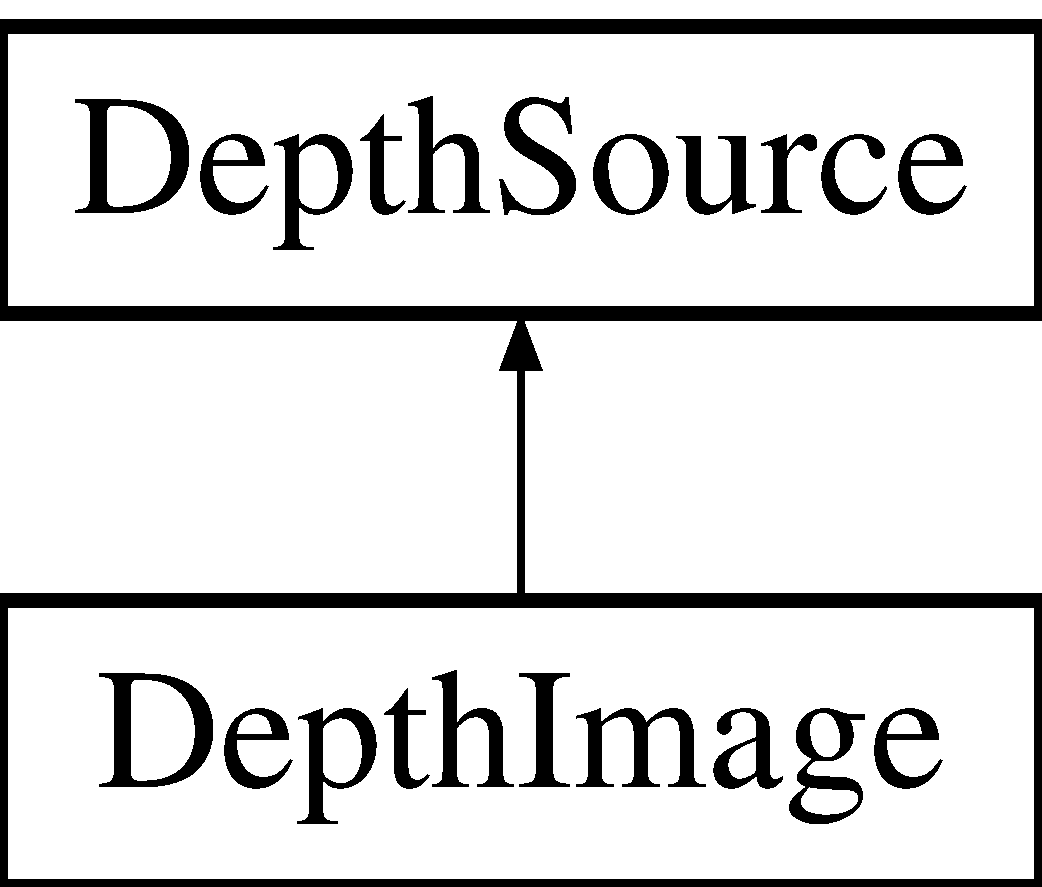
\includegraphics[height=2.000000cm]{classfovis_1_1DepthImage}
\end{center}
\end{figure}
\subsection*{Public Member Functions}
\begin{DoxyCompactItemize}
\item 
\hypertarget{classfovis_1_1DepthImage_ad14961dd8148a0bde0f129e38f05ce05}{
{\bfseries DepthImage} (const \hyperlink{structfovis_1_1CameraIntrinsicsParameters}{CameraIntrinsicsParameters} \&rgb\_\-camera\_\-params, int depth\_\-width, int depth\_\-height)}
\label{classfovis_1_1DepthImage_ad14961dd8148a0bde0f129e38f05ce05}

\item 
virtual double \hyperlink{classfovis_1_1DepthImage_a5429ab9acd4e4f8d154c952ff95b1149}{getBaseline} () const 
\item 
virtual void \hyperlink{classfovis_1_1DepthImage_a0b83e0c45768e90787bc7f0c2c77606d}{getXyz} (\hyperlink{classfovis_1_1OdometryFrame}{OdometryFrame} $\ast$frame)
\item 
virtual bool \hyperlink{classfovis_1_1DepthImage_ab94d0972d755837688cfc95aa144a6e1}{haveXyz} (int u, int v)
\item 
virtual void \hyperlink{classfovis_1_1DepthImage_ad0922053f71946f74bc26225848010e6}{refineXyz} (\hyperlink{classfovis_1_1FeatureMatch}{FeatureMatch} $\ast$matches, int num\_\-matches, \hyperlink{classfovis_1_1OdometryFrame}{OdometryFrame} $\ast$frame)
\item 
void \hyperlink{classfovis_1_1DepthImage_a02865b6272767324308c9b912d65a466}{setDepthImage} (const float $\ast$depth\_\-data)
\end{DoxyCompactItemize}


\subsection{Detailed Description}
Depth source where a fully dense, metric depth image is available. 

TODO 

\subsection{Member Function Documentation}
\hypertarget{classfovis_1_1DepthImage_a02865b6272767324308c9b912d65a466}{
\index{fovis::DepthImage@{fovis::DepthImage}!setDepthImage@{setDepthImage}}
\index{setDepthImage@{setDepthImage}!fovis::DepthImage@{fovis::DepthImage}}
\subsubsection[{setDepthImage}]{\setlength{\rightskip}{0pt plus 5cm}void setDepthImage (
\begin{DoxyParamCaption}
\item[{const float $\ast$}]{depth\_\-data}
\end{DoxyParamCaption}
)}}
\label{classfovis_1_1DepthImage_a02865b6272767324308c9b912d65a466}
Set the depth image, a width x height array of distances, units given in meters. Each pixel of the depth image corresponds to a point in the rectified RGB image. \hypertarget{classfovis_1_1DepthImage_ab94d0972d755837688cfc95aa144a6e1}{
\index{fovis::DepthImage@{fovis::DepthImage}!haveXyz@{haveXyz}}
\index{haveXyz@{haveXyz}!fovis::DepthImage@{fovis::DepthImage}}
\subsubsection[{haveXyz}]{\setlength{\rightskip}{0pt plus 5cm}virtual bool haveXyz (
\begin{DoxyParamCaption}
\item[{int}]{u, }
\item[{int}]{v}
\end{DoxyParamCaption}
)\hspace{0.3cm}{\ttfamily  \mbox{[}virtual\mbox{]}}}}
\label{classfovis_1_1DepthImage_ab94d0972d755837688cfc95aa144a6e1}
This should return true if it's not certain there's no depth at (u,v). It should be an inexpensive check that is used to avoid pointless (hah!) creation of keypoints. False positives are fine as ling as getXyz gets rid of them. 

Implements \hyperlink{classfovis_1_1DepthSource_ad0d2b9dd0e48e428319c3c84e87fa5cf}{DepthSource}.

\hypertarget{classfovis_1_1DepthImage_a0b83e0c45768e90787bc7f0c2c77606d}{
\index{fovis::DepthImage@{fovis::DepthImage}!getXyz@{getXyz}}
\index{getXyz@{getXyz}!fovis::DepthImage@{fovis::DepthImage}}
\subsubsection[{getXyz}]{\setlength{\rightskip}{0pt plus 5cm}virtual void getXyz (
\begin{DoxyParamCaption}
\item[{{\bf OdometryFrame} $\ast$}]{frame}
\end{DoxyParamCaption}
)\hspace{0.3cm}{\ttfamily  \mbox{[}virtual\mbox{]}}}}
\label{classfovis_1_1DepthImage_a0b83e0c45768e90787bc7f0c2c77606d}
Populate keypoints in frame with XYZ data. 

Implements \hyperlink{classfovis_1_1DepthSource_a0259f77a02ba85f5370407db4759d16a}{DepthSource}.

\hypertarget{classfovis_1_1DepthImage_ad0922053f71946f74bc26225848010e6}{
\index{fovis::DepthImage@{fovis::DepthImage}!refineXyz@{refineXyz}}
\index{refineXyz@{refineXyz}!fovis::DepthImage@{fovis::DepthImage}}
\subsubsection[{refineXyz}]{\setlength{\rightskip}{0pt plus 5cm}virtual void refineXyz (
\begin{DoxyParamCaption}
\item[{{\bf FeatureMatch} $\ast$}]{matches, }
\item[{int}]{num\_\-matches, }
\item[{{\bf OdometryFrame} $\ast$}]{frame}
\end{DoxyParamCaption}
)\hspace{0.3cm}{\ttfamily  \mbox{[}virtual\mbox{]}}}}
\label{classfovis_1_1DepthImage_ad0922053f71946f74bc26225848010e6}
Refine XYZ data of target keypoints in matches (usually after subpixel refinement of the matches across time). 

Implements \hyperlink{classfovis_1_1DepthSource_a4d6eafb84371d0720cd7ee53ac2e659a}{DepthSource}.

\hypertarget{classfovis_1_1DepthImage_a5429ab9acd4e4f8d154c952ff95b1149}{
\index{fovis::DepthImage@{fovis::DepthImage}!getBaseline@{getBaseline}}
\index{getBaseline@{getBaseline}!fovis::DepthImage@{fovis::DepthImage}}
\subsubsection[{getBaseline}]{\setlength{\rightskip}{0pt plus 5cm}virtual double getBaseline (
\begin{DoxyParamCaption}
{}
\end{DoxyParamCaption}
) const\hspace{0.3cm}{\ttfamily  \mbox{[}inline, virtual\mbox{]}}}}
\label{classfovis_1_1DepthImage_a5429ab9acd4e4f8d154c952ff95b1149}
Return baseline of depth source, if applicable. If not applicable (e.g. for OpenNI devices) return 0. 

Implements \hyperlink{classfovis_1_1DepthSource_a22d76295f183f3ec9e34d2d7e837c675}{DepthSource}.



The documentation for this class was generated from the following file:\begin{DoxyCompactItemize}
\item 
depth\_\-image.hpp\end{DoxyCompactItemize}

\hypertarget{classfovis_1_1DepthSource}{
\section{DepthSource Class Reference}
\label{classfovis_1_1DepthSource}\index{fovis::DepthSource@{fovis::DepthSource}}
}


Provides depth estimates for input image pixels.  


Inheritance diagram for DepthSource:\begin{figure}[H]
\begin{center}
\leavevmode
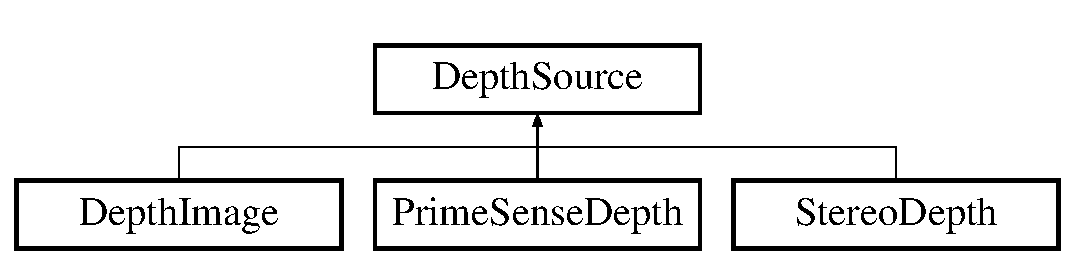
\includegraphics[height=2.000000cm]{classfovis_1_1DepthSource}
\end{center}
\end{figure}
\subsection*{Public Member Functions}
\begin{DoxyCompactItemize}
\item 
virtual double \hyperlink{classfovis_1_1DepthSource_a22d76295f183f3ec9e34d2d7e837c675}{getBaseline} () const =0
\item 
virtual void \hyperlink{classfovis_1_1DepthSource_a0259f77a02ba85f5370407db4759d16a}{getXyz} (\hyperlink{classfovis_1_1OdometryFrame}{OdometryFrame} $\ast$frame)=0
\item 
virtual bool \hyperlink{classfovis_1_1DepthSource_ad0d2b9dd0e48e428319c3c84e87fa5cf}{haveXyz} (int u, int v)=0
\item 
virtual void \hyperlink{classfovis_1_1DepthSource_a4d6eafb84371d0720cd7ee53ac2e659a}{refineXyz} (\hyperlink{classfovis_1_1FeatureMatch}{FeatureMatch} $\ast$matches, int num\_\-matches, \hyperlink{classfovis_1_1OdometryFrame}{OdometryFrame} $\ast$frame)=0
\end{DoxyCompactItemize}


\subsection{Detailed Description}
Provides depth estimates for input image pixels. 

A reliable source of depth estimates at as many pixels in an image as possible is crucial to producing useful visual odometry estimates. The \hyperlink{classfovis_1_1DepthSource}{DepthSource} class abstracts out the process of determining depth at each pixel.

\hyperlink{classfovis_1_1DepthSource}{DepthSource} is used in a lazy fashion. First, keypoints in the input image are identified. Next, keypoints without depth information are filtered out (pixels where \hyperlink{classfovis_1_1DepthSource_ad0d2b9dd0e48e428319c3c84e87fa5cf}{haveXyz()} returns false) and discarded. Later, the actual depth of the remaining keypoints is retrieved using \hyperlink{classfovis_1_1DepthSource_a0259f77a02ba85f5370407db4759d16a}{getXyz()}. Finally, after features are temporally matched across frames and their keypoint positions refined, \hyperlink{classfovis_1_1DepthSource}{DepthSource} is used again to refine the depth estimates of the refined keypoint image positions. 

\subsection{Member Function Documentation}
\hypertarget{classfovis_1_1DepthSource_ad0d2b9dd0e48e428319c3c84e87fa5cf}{
\index{fovis::DepthSource@{fovis::DepthSource}!haveXyz@{haveXyz}}
\index{haveXyz@{haveXyz}!fovis::DepthSource@{fovis::DepthSource}}
\subsubsection[{haveXyz}]{\setlength{\rightskip}{0pt plus 5cm}virtual bool haveXyz (
\begin{DoxyParamCaption}
\item[{int}]{u, }
\item[{int}]{v}
\end{DoxyParamCaption}
)\hspace{0.3cm}{\ttfamily  \mbox{[}pure virtual\mbox{]}}}}
\label{classfovis_1_1DepthSource_ad0d2b9dd0e48e428319c3c84e87fa5cf}
This should return true if it's not certain there's no depth at (u,v). It should be an inexpensive check that is used to avoid pointless (hah!) creation of keypoints. False positives are fine as ling as getXyz gets rid of them. 

Implemented in \hyperlink{classfovis_1_1DepthImage_ab94d0972d755837688cfc95aa144a6e1}{DepthImage}, \hyperlink{classfovis_1_1PrimeSenseDepth_af5915074d7b5e0694bcb0fae662c6c6c}{PrimeSenseDepth}, and \hyperlink{classfovis_1_1StereoDepth_ab94d0972d755837688cfc95aa144a6e1}{StereoDepth}.

\hypertarget{classfovis_1_1DepthSource_a0259f77a02ba85f5370407db4759d16a}{
\index{fovis::DepthSource@{fovis::DepthSource}!getXyz@{getXyz}}
\index{getXyz@{getXyz}!fovis::DepthSource@{fovis::DepthSource}}
\subsubsection[{getXyz}]{\setlength{\rightskip}{0pt plus 5cm}virtual void getXyz (
\begin{DoxyParamCaption}
\item[{{\bf OdometryFrame} $\ast$}]{frame}
\end{DoxyParamCaption}
)\hspace{0.3cm}{\ttfamily  \mbox{[}pure virtual\mbox{]}}}}
\label{classfovis_1_1DepthSource_a0259f77a02ba85f5370407db4759d16a}
Populate keypoints in frame with XYZ data. 

Implemented in \hyperlink{classfovis_1_1DepthImage_a0b83e0c45768e90787bc7f0c2c77606d}{DepthImage}, \hyperlink{classfovis_1_1PrimeSenseDepth_a9ba60dfd976745761bb861f08a374679}{PrimeSenseDepth}, and \hyperlink{classfovis_1_1StereoDepth_a0b83e0c45768e90787bc7f0c2c77606d}{StereoDepth}.

\hypertarget{classfovis_1_1DepthSource_a4d6eafb84371d0720cd7ee53ac2e659a}{
\index{fovis::DepthSource@{fovis::DepthSource}!refineXyz@{refineXyz}}
\index{refineXyz@{refineXyz}!fovis::DepthSource@{fovis::DepthSource}}
\subsubsection[{refineXyz}]{\setlength{\rightskip}{0pt plus 5cm}virtual void refineXyz (
\begin{DoxyParamCaption}
\item[{{\bf FeatureMatch} $\ast$}]{matches, }
\item[{int}]{num\_\-matches, }
\item[{{\bf OdometryFrame} $\ast$}]{frame}
\end{DoxyParamCaption}
)\hspace{0.3cm}{\ttfamily  \mbox{[}pure virtual\mbox{]}}}}
\label{classfovis_1_1DepthSource_a4d6eafb84371d0720cd7ee53ac2e659a}
Refine XYZ data of target keypoints in matches (usually after subpixel refinement of the matches across time). 

Implemented in \hyperlink{classfovis_1_1DepthImage_ad0922053f71946f74bc26225848010e6}{DepthImage}, \hyperlink{classfovis_1_1PrimeSenseDepth_a39e83560fd704306d53858d07d61621b}{PrimeSenseDepth}, and \hyperlink{classfovis_1_1StereoDepth_ad0922053f71946f74bc26225848010e6}{StereoDepth}.

\hypertarget{classfovis_1_1DepthSource_a22d76295f183f3ec9e34d2d7e837c675}{
\index{fovis::DepthSource@{fovis::DepthSource}!getBaseline@{getBaseline}}
\index{getBaseline@{getBaseline}!fovis::DepthSource@{fovis::DepthSource}}
\subsubsection[{getBaseline}]{\setlength{\rightskip}{0pt plus 5cm}virtual double getBaseline (
\begin{DoxyParamCaption}
{}
\end{DoxyParamCaption}
) const\hspace{0.3cm}{\ttfamily  \mbox{[}pure virtual\mbox{]}}}}
\label{classfovis_1_1DepthSource_a22d76295f183f3ec9e34d2d7e837c675}
Return baseline of depth source, if applicable. If not applicable (e.g. for OpenNI devices) return 0. 

Implemented in \hyperlink{classfovis_1_1DepthImage_a5429ab9acd4e4f8d154c952ff95b1149}{DepthImage}, \hyperlink{classfovis_1_1PrimeSenseDepth_a1941b0a011e836e922ce08cf48c635f9}{PrimeSenseDepth}, and \hyperlink{classfovis_1_1StereoDepth_a5429ab9acd4e4f8d154c952ff95b1149}{StereoDepth}.



The documentation for this class was generated from the following file:\begin{DoxyCompactItemize}
\item 
depth\_\-source.hpp\end{DoxyCompactItemize}

\hypertarget{classfovis_1_1FeatureMatch}{
\section{FeatureMatch Class Reference}
\label{classfovis_1_1FeatureMatch}\index{fovis::FeatureMatch@{fovis::FeatureMatch}}
}


Represents a single image feature matched between two camera images taken at different times.  


\subsection*{Public Member Functions}
\begin{DoxyCompactItemize}
\item 
\hyperlink{classfovis_1_1FeatureMatch_adccc0fc6e6b8100d71bd31cfcb9ae745}{FeatureMatch} ()
\item 
\hyperlink{classfovis_1_1FeatureMatch_a3c2499c4698d2dc6ae72224524aa693a}{FeatureMatch} (\hyperlink{classfovis_1_1KeypointData}{KeypointData} $\ast$\hyperlink{classfovis_1_1FeatureMatch_a85a2bf617b8f5152083f5acda254a61c}{target\_\-keypoint}, \hyperlink{classfovis_1_1KeypointData}{KeypointData} $\ast$\hyperlink{classfovis_1_1FeatureMatch_a63211a4e001cec95acf8363b81af1216}{ref\_\-keypoint})
\end{DoxyCompactItemize}
\subsection*{Public Attributes}
\begin{DoxyCompactItemize}
\item 
int \hyperlink{classfovis_1_1FeatureMatch_ae5fb6416f0d1fa278a22570505e05e13}{compatibility\_\-degree}
\item 
std::vector$<$ int $>$ \hyperlink{classfovis_1_1FeatureMatch_a92a84284bf0e8709364e0250c1063257}{consistency\_\-vec}
\item 
int \hyperlink{classfovis_1_1FeatureMatch_a7441ef0865bcb3db9b8064dd7375c1ea}{id}
\item 
bool \hyperlink{classfovis_1_1FeatureMatch_ab94bc799c5558ad8bcc29d94b478f292}{in\_\-maximal\_\-clique}
\item 
bool \hyperlink{classfovis_1_1FeatureMatch_af5eefbf5c8382030e20e4a7ae064987f}{inlier}
\item 
\hyperlink{classfovis_1_1KeypointData}{KeypointData} $\ast$ \hyperlink{classfovis_1_1FeatureMatch_a63211a4e001cec95acf8363b81af1216}{ref\_\-keypoint}
\item 
\hyperlink{classfovis_1_1KeypointData}{KeypointData} \hyperlink{classfovis_1_1FeatureMatch_ac7bde8fda75951ab16ca9ed8adfe2118}{refined\_\-target\_\-keypoint}
\item 
double \hyperlink{classfovis_1_1FeatureMatch_aed648d3f72076806d79f7c4c78151487}{reprojection\_\-error}
\item 
MatchStatusCode \hyperlink{classfovis_1_1FeatureMatch_a5a17170db3bee9a227cb28782b9532a7}{status}
\item 
\hyperlink{classfovis_1_1KeypointData}{KeypointData} $\ast$ \hyperlink{classfovis_1_1FeatureMatch_a85a2bf617b8f5152083f5acda254a61c}{target\_\-keypoint}
\item 
int \hyperlink{classfovis_1_1FeatureMatch_a8e64acfab4c3eba5b36eb3b6f15b9434}{track\_\-id}
\end{DoxyCompactItemize}


\subsection{Detailed Description}
Represents a single image feature matched between two camera images taken at different times. 

The two frames are referred to as the reference and target frames. 

\subsection{Constructor \& Destructor Documentation}
\hypertarget{classfovis_1_1FeatureMatch_adccc0fc6e6b8100d71bd31cfcb9ae745}{
\index{fovis::FeatureMatch@{fovis::FeatureMatch}!FeatureMatch@{FeatureMatch}}
\index{FeatureMatch@{FeatureMatch}!fovis::FeatureMatch@{fovis::FeatureMatch}}
\subsubsection[{FeatureMatch}]{\setlength{\rightskip}{0pt plus 5cm}{\bf FeatureMatch} (
\begin{DoxyParamCaption}
{}
\end{DoxyParamCaption}
)\hspace{0.3cm}{\ttfamily  \mbox{[}inline\mbox{]}}}}
\label{classfovis_1_1FeatureMatch_adccc0fc6e6b8100d71bd31cfcb9ae745}
Initializes a NULL (and useless) feature match. \hypertarget{classfovis_1_1FeatureMatch_a3c2499c4698d2dc6ae72224524aa693a}{
\index{fovis::FeatureMatch@{fovis::FeatureMatch}!FeatureMatch@{FeatureMatch}}
\index{FeatureMatch@{FeatureMatch}!fovis::FeatureMatch@{fovis::FeatureMatch}}
\subsubsection[{FeatureMatch}]{\setlength{\rightskip}{0pt plus 5cm}{\bf FeatureMatch} (
\begin{DoxyParamCaption}
\item[{{\bf KeypointData} $\ast$}]{target\_\-keypoint, }
\item[{{\bf KeypointData} $\ast$}]{ref\_\-keypoint}
\end{DoxyParamCaption}
)\hspace{0.3cm}{\ttfamily  \mbox{[}inline\mbox{]}}}}
\label{classfovis_1_1FeatureMatch_a3c2499c4698d2dc6ae72224524aa693a}
Initializes a feature match from a target and reference keypoint. 

\subsection{Member Data Documentation}
\hypertarget{classfovis_1_1FeatureMatch_a85a2bf617b8f5152083f5acda254a61c}{
\index{fovis::FeatureMatch@{fovis::FeatureMatch}!target\_\-keypoint@{target\_\-keypoint}}
\index{target\_\-keypoint@{target\_\-keypoint}!fovis::FeatureMatch@{fovis::FeatureMatch}}
\subsubsection[{target\_\-keypoint}]{\setlength{\rightskip}{0pt plus 5cm}{\bf KeypointData}$\ast$ {\bf target\_\-keypoint}}}
\label{classfovis_1_1FeatureMatch_a85a2bf617b8f5152083f5acda254a61c}
The target keypoint. \hypertarget{classfovis_1_1FeatureMatch_a63211a4e001cec95acf8363b81af1216}{
\index{fovis::FeatureMatch@{fovis::FeatureMatch}!ref\_\-keypoint@{ref\_\-keypoint}}
\index{ref\_\-keypoint@{ref\_\-keypoint}!fovis::FeatureMatch@{fovis::FeatureMatch}}
\subsubsection[{ref\_\-keypoint}]{\setlength{\rightskip}{0pt plus 5cm}{\bf KeypointData}$\ast$ {\bf ref\_\-keypoint}}}
\label{classfovis_1_1FeatureMatch_a63211a4e001cec95acf8363b81af1216}
The reference keypoint. \hypertarget{classfovis_1_1FeatureMatch_ac7bde8fda75951ab16ca9ed8adfe2118}{
\index{fovis::FeatureMatch@{fovis::FeatureMatch}!refined\_\-target\_\-keypoint@{refined\_\-target\_\-keypoint}}
\index{refined\_\-target\_\-keypoint@{refined\_\-target\_\-keypoint}!fovis::FeatureMatch@{fovis::FeatureMatch}}
\subsubsection[{refined\_\-target\_\-keypoint}]{\setlength{\rightskip}{0pt plus 5cm}{\bf KeypointData} {\bf refined\_\-target\_\-keypoint}}}
\label{classfovis_1_1FeatureMatch_ac7bde8fda75951ab16ca9ed8adfe2118}
The target keypoint, after subpixel refinement of the feature match in image space. \hypertarget{classfovis_1_1FeatureMatch_a92a84284bf0e8709364e0250c1063257}{
\index{fovis::FeatureMatch@{fovis::FeatureMatch}!consistency\_\-vec@{consistency\_\-vec}}
\index{consistency\_\-vec@{consistency\_\-vec}!fovis::FeatureMatch@{fovis::FeatureMatch}}
\subsubsection[{consistency\_\-vec}]{\setlength{\rightskip}{0pt plus 5cm}std::vector$<$int$>$ {\bf consistency\_\-vec}}}
\label{classfovis_1_1FeatureMatch_a92a84284bf0e8709364e0250c1063257}
binary vector, one entry for every feature match. Each entry is 1 if the motion according to this match is compatible with the motion according to the other match. \hypertarget{classfovis_1_1FeatureMatch_ae5fb6416f0d1fa278a22570505e05e13}{
\index{fovis::FeatureMatch@{fovis::FeatureMatch}!compatibility\_\-degree@{compatibility\_\-degree}}
\index{compatibility\_\-degree@{compatibility\_\-degree}!fovis::FeatureMatch@{fovis::FeatureMatch}}
\subsubsection[{compatibility\_\-degree}]{\setlength{\rightskip}{0pt plus 5cm}int {\bf compatibility\_\-degree}}}
\label{classfovis_1_1FeatureMatch_ae5fb6416f0d1fa278a22570505e05e13}
number of 1s in consistency\_\-vec \hypertarget{classfovis_1_1FeatureMatch_ab94bc799c5558ad8bcc29d94b478f292}{
\index{fovis::FeatureMatch@{fovis::FeatureMatch}!in\_\-maximal\_\-clique@{in\_\-maximal\_\-clique}}
\index{in\_\-maximal\_\-clique@{in\_\-maximal\_\-clique}!fovis::FeatureMatch@{fovis::FeatureMatch}}
\subsubsection[{in\_\-maximal\_\-clique}]{\setlength{\rightskip}{0pt plus 5cm}bool {\bf in\_\-maximal\_\-clique}}}
\label{classfovis_1_1FeatureMatch_ab94bc799c5558ad8bcc29d94b478f292}
Is this feature match in the maximal consistency clique \hypertarget{classfovis_1_1FeatureMatch_af5eefbf5c8382030e20e4a7ae064987f}{
\index{fovis::FeatureMatch@{fovis::FeatureMatch}!inlier@{inlier}}
\index{inlier@{inlier}!fovis::FeatureMatch@{fovis::FeatureMatch}}
\subsubsection[{inlier}]{\setlength{\rightskip}{0pt plus 5cm}bool {\bf inlier}}}
\label{classfovis_1_1FeatureMatch_af5eefbf5c8382030e20e4a7ae064987f}
Is this feature an inlier, used for motion estimation \hypertarget{classfovis_1_1FeatureMatch_a7441ef0865bcb3db9b8064dd7375c1ea}{
\index{fovis::FeatureMatch@{fovis::FeatureMatch}!id@{id}}
\index{id@{id}!fovis::FeatureMatch@{fovis::FeatureMatch}}
\subsubsection[{id}]{\setlength{\rightskip}{0pt plus 5cm}int {\bf id}}}
\label{classfovis_1_1FeatureMatch_a7441ef0865bcb3db9b8064dd7375c1ea}
Identifies the match during outlier rejection. \hypertarget{classfovis_1_1FeatureMatch_aed648d3f72076806d79f7c4c78151487}{
\index{fovis::FeatureMatch@{fovis::FeatureMatch}!reprojection\_\-error@{reprojection\_\-error}}
\index{reprojection\_\-error@{reprojection\_\-error}!fovis::FeatureMatch@{fovis::FeatureMatch}}
\subsubsection[{reprojection\_\-error}]{\setlength{\rightskip}{0pt plus 5cm}double {\bf reprojection\_\-error}}}
\label{classfovis_1_1FeatureMatch_aed648d3f72076806d79f7c4c78151487}
The image-\/space distance between the reference keypoint and the target keypoint reprojected onto the reference image. \hypertarget{classfovis_1_1FeatureMatch_a8e64acfab4c3eba5b36eb3b6f15b9434}{
\index{fovis::FeatureMatch@{fovis::FeatureMatch}!track\_\-id@{track\_\-id}}
\index{track\_\-id@{track\_\-id}!fovis::FeatureMatch@{fovis::FeatureMatch}}
\subsubsection[{track\_\-id}]{\setlength{\rightskip}{0pt plus 5cm}int {\bf track\_\-id}}}
\label{classfovis_1_1FeatureMatch_a8e64acfab4c3eba5b36eb3b6f15b9434}
Identifies the feature track externally. If a feature in a new frame is matched to a feature in the previous frame, then the corresponding \hyperlink{classfovis_1_1FeatureMatch}{FeatureMatch} object takes on the track\_\-id value of the \hyperlink{classfovis_1_1FeatureMatch}{FeatureMatch} object for the previous frame feature. If the previous frame feature is new (i.e., wasn't matched to a feature in the previous-\/previous frame), then the track\_\-id is set to a new value. \hypertarget{classfovis_1_1FeatureMatch_a5a17170db3bee9a227cb28782b9532a7}{
\index{fovis::FeatureMatch@{fovis::FeatureMatch}!status@{status}}
\index{status@{status}!fovis::FeatureMatch@{fovis::FeatureMatch}}
\subsubsection[{status}]{\setlength{\rightskip}{0pt plus 5cm}MatchStatusCode {\bf status}}}
\label{classfovis_1_1FeatureMatch_a5a17170db3bee9a227cb28782b9532a7}
status of the feature match. Value is one of: {\ttfamily MATCH\_\-NEEDS\_\-DEPTH\_\-REFINEMENT}, {\ttfamily MATCH\_\-OK}, or {\ttfamily MATCH\_\-REFINEMENT\_\-FAILED}. 

The documentation for this class was generated from the following file:\begin{DoxyCompactItemize}
\item 
feature\_\-match.hpp\end{DoxyCompactItemize}

\hypertarget{classfovis_1_1FeatureMatcher}{
\section{FeatureMatcher Class Reference}
\label{classfovis_1_1FeatureMatcher}\index{fovis::FeatureMatcher@{fovis::FeatureMatcher}}
}


Matches features between a reference and a target image.  


\subsection*{Public Member Functions}
\begin{DoxyCompactItemize}
\item 
void \hyperlink{classfovis_1_1FeatureMatcher_a3f102d9c195b071349c7f18365a05287}{matchFeatures} (\hyperlink{classfovis_1_1PyramidLevel}{PyramidLevel} $\ast$ref\_\-level, \hyperlink{classfovis_1_1PyramidLevel}{PyramidLevel} $\ast$target\_\-level, const std::vector$<$ std::vector$<$ int $>$ $>$ \&candidates, \hyperlink{classfovis_1_1FeatureMatch}{FeatureMatch} $\ast$matches, int $\ast$num\_\-matches)
\end{DoxyCompactItemize}


\subsection{Detailed Description}
Matches features between a reference and a target image. 

\subsection{Member Function Documentation}
\hypertarget{classfovis_1_1FeatureMatcher_a3f102d9c195b071349c7f18365a05287}{
\index{fovis::FeatureMatcher@{fovis::FeatureMatcher}!matchFeatures@{matchFeatures}}
\index{matchFeatures@{matchFeatures}!fovis::FeatureMatcher@{fovis::FeatureMatcher}}
\subsubsection[{matchFeatures}]{\setlength{\rightskip}{0pt plus 5cm}void matchFeatures (
\begin{DoxyParamCaption}
\item[{{\bf PyramidLevel} $\ast$}]{ref\_\-level, }
\item[{{\bf PyramidLevel} $\ast$}]{target\_\-level, }
\item[{const std::vector$<$ std::vector$<$ int $>$ $>$ \&}]{candidates, }
\item[{{\bf FeatureMatch} $\ast$}]{matches, }
\item[{int $\ast$}]{num\_\-matches}
\end{DoxyParamCaption}
)}}
\label{classfovis_1_1FeatureMatcher_a3f102d9c195b071349c7f18365a05287}
Feature matching using sum of absolute differences (\hyperlink{classfovis_1_1SAD}{SAD}).


\begin{DoxyParams}{Parameters}
{\em ref\_\-level} & features in the reference image. \\
\hline
{\em target\_\-level} & features in the target image. \\
\hline
{\em candidates} & identifies potential match candidates for each feature in the reference image. For every reference feature, there is a vector of target feature indices that is a potential match. \\
\hline
{\em matches} & output array of matches. This should be pre-\/allocated and of size at least min(num features in {\ttfamily ref\_\-level}, num features in {\ttfamily target\_\-level}) \\
\hline
{\em num\_\-matches} & output parameter, is set to the number of features matched. \\
\hline
\end{DoxyParams}


The documentation for this class was generated from the following file:\begin{DoxyCompactItemize}
\item 
feature\_\-matcher.hpp\end{DoxyCompactItemize}

\hypertarget{classfovis_1_1GridKeyPointFilter}{
\section{GridKeyPointFilter Class Reference}
\label{classfovis_1_1GridKeyPointFilter}\index{fovis::GridKeyPointFilter@{fovis::GridKeyPointFilter}}
}


Places features into grid cells and discards the weakest features in each cell.  


\subsection*{Public Member Functions}
\begin{DoxyCompactItemize}
\item 
void \hyperlink{classfovis_1_1GridKeyPointFilter_af5f860867a8c45901c2b56cb208742f9}{filter} (std::vector$<$ \hyperlink{classfovis_1_1KeyPoint}{KeyPoint} $>$ $\ast$keypoints)
\item 
\hyperlink{classfovis_1_1GridKeyPointFilter_a8f2d11b65b3438c4594e6a55ae8ab942}{GridKeyPointFilter} (int img\_\-width, int img\_\-height, int bucket\_\-width, int bucket\_\-height, int max\_\-keypoints\_\-per\_\-bucket)
\end{DoxyCompactItemize}


\subsection{Detailed Description}
Places features into grid cells and discards the weakest features in each cell. 

\subsection{Constructor \& Destructor Documentation}
\hypertarget{classfovis_1_1GridKeyPointFilter_a8f2d11b65b3438c4594e6a55ae8ab942}{
\index{fovis::GridKeyPointFilter@{fovis::GridKeyPointFilter}!GridKeyPointFilter@{GridKeyPointFilter}}
\index{GridKeyPointFilter@{GridKeyPointFilter}!fovis::GridKeyPointFilter@{fovis::GridKeyPointFilter}}
\subsubsection[{GridKeyPointFilter}]{\setlength{\rightskip}{0pt plus 5cm}{\bf GridKeyPointFilter} (
\begin{DoxyParamCaption}
\item[{int}]{img\_\-width, }
\item[{int}]{img\_\-height, }
\item[{int}]{bucket\_\-width, }
\item[{int}]{bucket\_\-height, }
\item[{int}]{max\_\-keypoints\_\-per\_\-bucket}
\end{DoxyParamCaption}
)\hspace{0.3cm}{\ttfamily  \mbox{[}inline\mbox{]}}}}
\label{classfovis_1_1GridKeyPointFilter_a8f2d11b65b3438c4594e6a55ae8ab942}
Construct a keypoint filter.

Conceptually, lays down a grid over the image and sorts keypoints into a grid cell based on their image locations. Then removes the weakest keypoints in each cell (using the Keypoint::score field) until there are at most {\ttfamily max\_\-keypoints\_\-per\_\-bucket} in each grid cell.


\begin{DoxyParams}{Parameters}
{\em img\_\-width} & the width of the input image. \\
\hline
{\em img\_\-height} & the height of the input image. \\
\hline
{\em bucket\_\-width} & the width of each bucket. \\
\hline
{\em bucket\_\-height} & the height of each bucket. \\
\hline
{\em max\_\-keypoints\_\-per\_\-bucket} & the maximum number of keypoints in each grid cell after filtering. \\
\hline
\end{DoxyParams}


\subsection{Member Function Documentation}
\hypertarget{classfovis_1_1GridKeyPointFilter_af5f860867a8c45901c2b56cb208742f9}{
\index{fovis::GridKeyPointFilter@{fovis::GridKeyPointFilter}!filter@{filter}}
\index{filter@{filter}!fovis::GridKeyPointFilter@{fovis::GridKeyPointFilter}}
\subsubsection[{filter}]{\setlength{\rightskip}{0pt plus 5cm}void filter (
\begin{DoxyParamCaption}
\item[{std::vector$<$ {\bf KeyPoint} $>$ $\ast$}]{keypoints}
\end{DoxyParamCaption}
)}}
\label{classfovis_1_1GridKeyPointFilter_af5f860867a8c45901c2b56cb208742f9}
filters the specified vector of keypoints.


\begin{DoxyParams}{Parameters}
{\em keypoints} & input/output parameter. On output, the weakest keypoints in each grid cell will have been removed from this vector. \\
\hline
\end{DoxyParams}


The documentation for this class was generated from the following file:\begin{DoxyCompactItemize}
\item 
grid\_\-filter.hpp\end{DoxyCompactItemize}

\hypertarget{classfovis_1_1InitialHomographyEstimator}{
\section{InitialHomographyEstimator Class Reference}
\label{classfovis_1_1InitialHomographyEstimator}\index{fovis::InitialHomographyEstimator@{fovis::InitialHomographyEstimator}}
}


Estimates a rough 2D homography registering two images.  


\subsection*{Public Member Functions}
\begin{DoxyCompactItemize}
\item 
void \hyperlink{classfovis_1_1InitialHomographyEstimator_aaa00392f56809e71fdeeb250cef2c323}{setTemplateImage} (const uint8\_\-t $\ast$grayData, int width, int height, int stride, int downsampleFactor)
\item 
void \hyperlink{classfovis_1_1InitialHomographyEstimator_a1b396c2110d51803d5993808b8c81fbf}{setTestImage} (const uint8\_\-t $\ast$grayData, int width, int height, int stride, int downsampleFactor)
\item 
Eigen::Matrix3f \hyperlink{classfovis_1_1InitialHomographyEstimator_a433869e74d5e2738425ff4292b4446bb}{track} (const Eigen::Matrix3f \&init\_\-H, int nIters, double $\ast$finalRMS)
\end{DoxyCompactItemize}


\subsection{Detailed Description}
Estimates a rough 2D homography registering two images. 

\subsection{Member Function Documentation}
\hypertarget{classfovis_1_1InitialHomographyEstimator_aaa00392f56809e71fdeeb250cef2c323}{
\index{fovis::InitialHomographyEstimator@{fovis::InitialHomographyEstimator}!setTemplateImage@{setTemplateImage}}
\index{setTemplateImage@{setTemplateImage}!fovis::InitialHomographyEstimator@{fovis::InitialHomographyEstimator}}
\subsubsection[{setTemplateImage}]{\setlength{\rightskip}{0pt plus 5cm}void setTemplateImage (
\begin{DoxyParamCaption}
\item[{const uint8\_\-t $\ast$}]{grayData, }
\item[{int}]{width, }
\item[{int}]{height, }
\item[{int}]{stride, }
\item[{int}]{downsampleFactor}
\end{DoxyParamCaption}
)}}
\label{classfovis_1_1InitialHomographyEstimator_aaa00392f56809e71fdeeb250cef2c323}
Set the template image to the passed in arguments. assumes the image data is row-\/major. The image will be downsampled by $ 1/2^{downsampleFactor} $ \hypertarget{classfovis_1_1InitialHomographyEstimator_a1b396c2110d51803d5993808b8c81fbf}{
\index{fovis::InitialHomographyEstimator@{fovis::InitialHomographyEstimator}!setTestImage@{setTestImage}}
\index{setTestImage@{setTestImage}!fovis::InitialHomographyEstimator@{fovis::InitialHomographyEstimator}}
\subsubsection[{setTestImage}]{\setlength{\rightskip}{0pt plus 5cm}void setTestImage (
\begin{DoxyParamCaption}
\item[{const uint8\_\-t $\ast$}]{grayData, }
\item[{int}]{width, }
\item[{int}]{height, }
\item[{int}]{stride, }
\item[{int}]{downsampleFactor}
\end{DoxyParamCaption}
)}}
\label{classfovis_1_1InitialHomographyEstimator_a1b396c2110d51803d5993808b8c81fbf}
Set the test image accordingly. The opimization will warp this image to match the template assumes the image data is row-\/major. The image will be downsampled by $ 1/2^{downsampleFactor} $ \hypertarget{classfovis_1_1InitialHomographyEstimator_a433869e74d5e2738425ff4292b4446bb}{
\index{fovis::InitialHomographyEstimator@{fovis::InitialHomographyEstimator}!track@{track}}
\index{track@{track}!fovis::InitialHomographyEstimator@{fovis::InitialHomographyEstimator}}
\subsubsection[{track}]{\setlength{\rightskip}{0pt plus 5cm}Eigen::Matrix3f track (
\begin{DoxyParamCaption}
\item[{const Eigen::Matrix3f \&}]{init\_\-H, }
\item[{int}]{nIters, }
\item[{double $\ast$}]{finalRMS}
\end{DoxyParamCaption}
)}}
\label{classfovis_1_1InitialHomographyEstimator_a433869e74d5e2738425ff4292b4446bb}
Run ESM to find the homography between the template and test images. These should have already been passed in using the methods \hyperlink{classfovis_1_1InitialHomographyEstimator_aaa00392f56809e71fdeeb250cef2c323}{setTemplateImage()}, and \hyperlink{classfovis_1_1InitialHomographyEstimator_a1b396c2110d51803d5993808b8c81fbf}{setTestImage()}. 

The documentation for this class was generated from the following file:\begin{DoxyCompactItemize}
\item 
initial\_\-homography\_\-estimation.hpp\end{DoxyCompactItemize}

\hypertarget{classfovis_1_1IntensityDescriptorExtractor}{
\section{IntensityDescriptorExtractor Class Reference}
\label{classfovis_1_1IntensityDescriptorExtractor}\index{fovis::IntensityDescriptorExtractor@{fovis::IntensityDescriptorExtractor}}
}


Extracts mean-\/normalized intensity patch around a pixel.  


\subsection*{Public Member Functions}
\begin{DoxyCompactItemize}
\item 
const int $\ast$ \hyperlink{classfovis_1_1IntensityDescriptorExtractor_acb4a60e9159801a3486dd6f2081cf346}{getDescriptorIndexOffsets} () const 
\item 
int \hyperlink{classfovis_1_1IntensityDescriptorExtractor_ace19c8012ae7eaa4db2f807167b165f9}{getDescriptorLength} () const 
\item 
int \hyperlink{classfovis_1_1IntensityDescriptorExtractor_ab19595fa4e4bb6716f9ed7fa38a297b2}{getDescriptorStride} () const 
\item 
\hyperlink{classfovis_1_1IntensityDescriptorExtractor_ae89b1246e1e1a199bfcf70ce8e194f97}{IntensityDescriptorExtractor} (int raw\_\-gray\_\-stride, int feature\_\-window\_\-size)
\item 
void \hyperlink{classfovis_1_1IntensityDescriptorExtractor_a6741482f67c7acc2bbc6a45aa3e562b4}{populateDescriptorAligned} (uint8\_\-t $\ast$image, int x, int y, uint8\_\-t $\ast$descriptor) const 
\item 
void \hyperlink{classfovis_1_1IntensityDescriptorExtractor_aa1ad51fea7d5c44c9d1588a821ebafcd}{populateDescriptorInterp} (uint8\_\-t $\ast$image, float x, float y, uint8\_\-t $\ast$descriptor) const 
\item 
void \hyperlink{classfovis_1_1IntensityDescriptorExtractor_a78ac9f581501370c62b5213ebba152fa}{populateDescriptorsAligned} (uint8\_\-t $\ast$image, const \hyperlink{classfovis_1_1KeypointData}{KeypointData} $\ast$keypoints, int num\_\-keypoints, uint8\_\-t $\ast$descriptors) const 
\item 
void \hyperlink{classfovis_1_1IntensityDescriptorExtractor_a6f626ae691f4031726a17453b3cce95c}{populateDescriptorsInterp} (uint8\_\-t $\ast$image, const \hyperlink{classfovis_1_1KeypointData}{KeypointData} $\ast$keypoints, int num\_\-keypoints, uint8\_\-t $\ast$descriptors) const 
\end{DoxyCompactItemize}


\subsection{Detailed Description}
Extracts mean-\/normalized intensity patch around a pixel. 

\subsection{Constructor \& Destructor Documentation}
\hypertarget{classfovis_1_1IntensityDescriptorExtractor_ae89b1246e1e1a199bfcf70ce8e194f97}{
\index{fovis::IntensityDescriptorExtractor@{fovis::IntensityDescriptorExtractor}!IntensityDescriptorExtractor@{IntensityDescriptorExtractor}}
\index{IntensityDescriptorExtractor@{IntensityDescriptorExtractor}!fovis::IntensityDescriptorExtractor@{fovis::IntensityDescriptorExtractor}}
\subsubsection[{IntensityDescriptorExtractor}]{\setlength{\rightskip}{0pt plus 5cm}{\bf IntensityDescriptorExtractor} (
\begin{DoxyParamCaption}
\item[{int}]{raw\_\-gray\_\-stride, }
\item[{int}]{feature\_\-window\_\-size}
\end{DoxyParamCaption}
)\hspace{0.3cm}{\ttfamily  \mbox{[}inline\mbox{]}}}}
\label{classfovis_1_1IntensityDescriptorExtractor_ae89b1246e1e1a199bfcf70ce8e194f97}

\begin{DoxyParams}{Parameters}
{\em raw\_\-gray\_\-stride} & specifies the number of bytes separating each row of the input image. \\
\hline
{\em feature\_\-window\_\-size} & the size of the descriptor window. \\
\hline
\end{DoxyParams}


\subsection{Member Function Documentation}
\hypertarget{classfovis_1_1IntensityDescriptorExtractor_aa1ad51fea7d5c44c9d1588a821ebafcd}{
\index{fovis::IntensityDescriptorExtractor@{fovis::IntensityDescriptorExtractor}!populateDescriptorInterp@{populateDescriptorInterp}}
\index{populateDescriptorInterp@{populateDescriptorInterp}!fovis::IntensityDescriptorExtractor@{fovis::IntensityDescriptorExtractor}}
\subsubsection[{populateDescriptorInterp}]{\setlength{\rightskip}{0pt plus 5cm}void populateDescriptorInterp (
\begin{DoxyParamCaption}
\item[{uint8\_\-t $\ast$}]{image, }
\item[{float}]{x, }
\item[{float}]{y, }
\item[{uint8\_\-t $\ast$}]{descriptor}
\end{DoxyParamCaption}
) const}}
\label{classfovis_1_1IntensityDescriptorExtractor_aa1ad51fea7d5c44c9d1588a821ebafcd}
Computes a single descriptor using bilinear interpolation at every point on the descriptor. This performs 4 floating point multiplications for every pixel in the descriptor.

Assumes that the output parameter {\ttfamily is} 16-\/byte aligned. \hypertarget{classfovis_1_1IntensityDescriptorExtractor_a6741482f67c7acc2bbc6a45aa3e562b4}{
\index{fovis::IntensityDescriptorExtractor@{fovis::IntensityDescriptorExtractor}!populateDescriptorAligned@{populateDescriptorAligned}}
\index{populateDescriptorAligned@{populateDescriptorAligned}!fovis::IntensityDescriptorExtractor@{fovis::IntensityDescriptorExtractor}}
\subsubsection[{populateDescriptorAligned}]{\setlength{\rightskip}{0pt plus 5cm}void populateDescriptorAligned (
\begin{DoxyParamCaption}
\item[{uint8\_\-t $\ast$}]{image, }
\item[{int}]{x, }
\item[{int}]{y, }
\item[{uint8\_\-t $\ast$}]{descriptor}
\end{DoxyParamCaption}
) const}}
\label{classfovis_1_1IntensityDescriptorExtractor_a6741482f67c7acc2bbc6a45aa3e562b4}
Computes a single descriptor. Assumes that the output parameter {\ttfamily descriptor} is 16-\/byte aligned. \hypertarget{classfovis_1_1IntensityDescriptorExtractor_a6f626ae691f4031726a17453b3cce95c}{
\index{fovis::IntensityDescriptorExtractor@{fovis::IntensityDescriptorExtractor}!populateDescriptorsInterp@{populateDescriptorsInterp}}
\index{populateDescriptorsInterp@{populateDescriptorsInterp}!fovis::IntensityDescriptorExtractor@{fovis::IntensityDescriptorExtractor}}
\subsubsection[{populateDescriptorsInterp}]{\setlength{\rightskip}{0pt plus 5cm}void populateDescriptorsInterp (
\begin{DoxyParamCaption}
\item[{uint8\_\-t $\ast$}]{image, }
\item[{const {\bf KeypointData} $\ast$}]{keypoints, }
\item[{int}]{num\_\-keypoints, }
\item[{uint8\_\-t $\ast$}]{descriptors}
\end{DoxyParamCaption}
) const}}
\label{classfovis_1_1IntensityDescriptorExtractor_a6f626ae691f4031726a17453b3cce95c}
Compute many descriptors using bilinear interpolation.


\begin{DoxyParams}{Parameters}
{\em image} & input image used for descriptor computation. \\
\hline
{\em keypoints} & keypoints for descriptor computation. \\
\hline
{\em num\_\-keypoints} & the number of keypoints. \\
\hline
{\em descriptors} & Must be 16-\/byte aligned and pre-\/allocated to {\ttfamily num\_\-keypoints} $\ast$ 16 $\ast$ \hyperlink{classfovis_1_1IntensityDescriptorExtractor_ab19595fa4e4bb6716f9ed7fa38a297b2}{getDescriptorStride()} bytes. \\
\hline
\end{DoxyParams}
\hypertarget{classfovis_1_1IntensityDescriptorExtractor_a78ac9f581501370c62b5213ebba152fa}{
\index{fovis::IntensityDescriptorExtractor@{fovis::IntensityDescriptorExtractor}!populateDescriptorsAligned@{populateDescriptorsAligned}}
\index{populateDescriptorsAligned@{populateDescriptorsAligned}!fovis::IntensityDescriptorExtractor@{fovis::IntensityDescriptorExtractor}}
\subsubsection[{populateDescriptorsAligned}]{\setlength{\rightskip}{0pt plus 5cm}void populateDescriptorsAligned (
\begin{DoxyParamCaption}
\item[{uint8\_\-t $\ast$}]{image, }
\item[{const {\bf KeypointData} $\ast$}]{keypoints, }
\item[{int}]{num\_\-keypoints, }
\item[{uint8\_\-t $\ast$}]{descriptors}
\end{DoxyParamCaption}
) const}}
\label{classfovis_1_1IntensityDescriptorExtractor_a78ac9f581501370c62b5213ebba152fa}
Compute many descriptors.


\begin{DoxyParams}{Parameters}
{\em image} & input image used for descriptor computation. \\
\hline
{\em keypoints} & keypoints for descriptor computation. \\
\hline
{\em num\_\-keypoints} & the number of keypoints. \\
\hline
{\em descriptors} & Must be 16-\/byte aligned and pre-\/allocated to {\ttfamily num\_\-keypoints} $\ast$ 16 $\ast$ \hyperlink{classfovis_1_1IntensityDescriptorExtractor_ab19595fa4e4bb6716f9ed7fa38a297b2}{getDescriptorStride()} bytes. \\
\hline
\end{DoxyParams}
\hypertarget{classfovis_1_1IntensityDescriptorExtractor_ab19595fa4e4bb6716f9ed7fa38a297b2}{
\index{fovis::IntensityDescriptorExtractor@{fovis::IntensityDescriptorExtractor}!getDescriptorStride@{getDescriptorStride}}
\index{getDescriptorStride@{getDescriptorStride}!fovis::IntensityDescriptorExtractor@{fovis::IntensityDescriptorExtractor}}
\subsubsection[{getDescriptorStride}]{\setlength{\rightskip}{0pt plus 5cm}int getDescriptorStride (
\begin{DoxyParamCaption}
{}
\end{DoxyParamCaption}
) const\hspace{0.3cm}{\ttfamily  \mbox{[}inline\mbox{]}}}}
\label{classfovis_1_1IntensityDescriptorExtractor_ab19595fa4e4bb6716f9ed7fa38a297b2}
\begin{DoxyReturn}{Returns}
the number of bytes that should separate descriptors in a vector of keypoint descriptors. This is usually a multiple of 16 so that each descriptor is 16-\/byte aligned. 
\end{DoxyReturn}
\hypertarget{classfovis_1_1IntensityDescriptorExtractor_acb4a60e9159801a3486dd6f2081cf346}{
\index{fovis::IntensityDescriptorExtractor@{fovis::IntensityDescriptorExtractor}!getDescriptorIndexOffsets@{getDescriptorIndexOffsets}}
\index{getDescriptorIndexOffsets@{getDescriptorIndexOffsets}!fovis::IntensityDescriptorExtractor@{fovis::IntensityDescriptorExtractor}}
\subsubsection[{getDescriptorIndexOffsets}]{\setlength{\rightskip}{0pt plus 5cm}const int$\ast$ getDescriptorIndexOffsets (
\begin{DoxyParamCaption}
{}
\end{DoxyParamCaption}
) const\hspace{0.3cm}{\ttfamily  \mbox{[}inline\mbox{]}}}}
\label{classfovis_1_1IntensityDescriptorExtractor_acb4a60e9159801a3486dd6f2081cf346}
\begin{DoxyReturn}{Returns}
an array of offset indices indicating the image offset of each descriptor pixel from the descriptor center pixel. 
\end{DoxyReturn}
\hypertarget{classfovis_1_1IntensityDescriptorExtractor_ace19c8012ae7eaa4db2f807167b165f9}{
\index{fovis::IntensityDescriptorExtractor@{fovis::IntensityDescriptorExtractor}!getDescriptorLength@{getDescriptorLength}}
\index{getDescriptorLength@{getDescriptorLength}!fovis::IntensityDescriptorExtractor@{fovis::IntensityDescriptorExtractor}}
\subsubsection[{getDescriptorLength}]{\setlength{\rightskip}{0pt plus 5cm}int getDescriptorLength (
\begin{DoxyParamCaption}
{}
\end{DoxyParamCaption}
) const\hspace{0.3cm}{\ttfamily  \mbox{[}inline\mbox{]}}}}
\label{classfovis_1_1IntensityDescriptorExtractor_ace19c8012ae7eaa4db2f807167b165f9}
\begin{DoxyReturn}{Returns}
the number of useful bytes in each descriptor. 
\end{DoxyReturn}


The documentation for this class was generated from the following file:\begin{DoxyCompactItemize}
\item 
intensity\_\-descriptor.hpp\end{DoxyCompactItemize}

\hypertarget{classfovis_1_1KeyPoint}{
\section{KeyPoint Class Reference}
\label{classfovis_1_1KeyPoint}\index{fovis::KeyPoint@{fovis::KeyPoint}}
}


An interesting point in an image.  


\subsection*{Public Member Functions}
\begin{DoxyCompactItemize}
\item 
\hyperlink{classfovis_1_1KeyPoint_a5c7501367f6f5207d0bf90916a8807f5}{KeyPoint} ()
\item 
\hyperlink{classfovis_1_1KeyPoint_a433f4b9f56afe421648c0bd16361a416}{KeyPoint} (float u\_\-, float v\_\-, float score\_\-)
\end{DoxyCompactItemize}
\subsection*{Public Attributes}
\begin{DoxyCompactItemize}
\item 
float \hyperlink{classfovis_1_1KeyPoint_a8c5cd9b525ee73a24b1d9d8e34982d1c}{score}
\item 
float \hyperlink{classfovis_1_1KeyPoint_a55831f7eab5ed2917a0191e858852f42}{u}
\item 
float \hyperlink{classfovis_1_1KeyPoint_a48d9522e58fa05906c6dba23e5745a72}{v}
\end{DoxyCompactItemize}


\subsection{Detailed Description}
An interesting point in an image. 

\subsection{Constructor \& Destructor Documentation}
\hypertarget{classfovis_1_1KeyPoint_a5c7501367f6f5207d0bf90916a8807f5}{
\index{fovis::KeyPoint@{fovis::KeyPoint}!KeyPoint@{KeyPoint}}
\index{KeyPoint@{KeyPoint}!fovis::KeyPoint@{fovis::KeyPoint}}
\subsubsection[{KeyPoint}]{\setlength{\rightskip}{0pt plus 5cm}{\bf KeyPoint} (
\begin{DoxyParamCaption}
{}
\end{DoxyParamCaption}
)\hspace{0.3cm}{\ttfamily  \mbox{[}inline\mbox{]}}}}
\label{classfovis_1_1KeyPoint_a5c7501367f6f5207d0bf90916a8807f5}
Initializes a keypoint to (0, 0) with score 0. \hypertarget{classfovis_1_1KeyPoint_a433f4b9f56afe421648c0bd16361a416}{
\index{fovis::KeyPoint@{fovis::KeyPoint}!KeyPoint@{KeyPoint}}
\index{KeyPoint@{KeyPoint}!fovis::KeyPoint@{fovis::KeyPoint}}
\subsubsection[{KeyPoint}]{\setlength{\rightskip}{0pt plus 5cm}{\bf KeyPoint} (
\begin{DoxyParamCaption}
\item[{float}]{u\_\-, }
\item[{float}]{v\_\-, }
\item[{float}]{score\_\-}
\end{DoxyParamCaption}
)\hspace{0.3cm}{\ttfamily  \mbox{[}inline\mbox{]}}}}
\label{classfovis_1_1KeyPoint_a433f4b9f56afe421648c0bd16361a416}
Initializes a keypoint to the specified coordinate and score. 

\subsection{Member Data Documentation}
\hypertarget{classfovis_1_1KeyPoint_a55831f7eab5ed2917a0191e858852f42}{
\index{fovis::KeyPoint@{fovis::KeyPoint}!u@{u}}
\index{u@{u}!fovis::KeyPoint@{fovis::KeyPoint}}
\subsubsection[{u}]{\setlength{\rightskip}{0pt plus 5cm}float {\bf u}}}
\label{classfovis_1_1KeyPoint_a55831f7eab5ed2917a0191e858852f42}
also known as the X coordinate. \hypertarget{classfovis_1_1KeyPoint_a48d9522e58fa05906c6dba23e5745a72}{
\index{fovis::KeyPoint@{fovis::KeyPoint}!v@{v}}
\index{v@{v}!fovis::KeyPoint@{fovis::KeyPoint}}
\subsubsection[{v}]{\setlength{\rightskip}{0pt plus 5cm}float {\bf v}}}
\label{classfovis_1_1KeyPoint_a48d9522e58fa05906c6dba23e5745a72}
also known as the Y coordinate. \hypertarget{classfovis_1_1KeyPoint_a8c5cd9b525ee73a24b1d9d8e34982d1c}{
\index{fovis::KeyPoint@{fovis::KeyPoint}!score@{score}}
\index{score@{score}!fovis::KeyPoint@{fovis::KeyPoint}}
\subsubsection[{score}]{\setlength{\rightskip}{0pt plus 5cm}float {\bf score}}}
\label{classfovis_1_1KeyPoint_a8c5cd9b525ee73a24b1d9d8e34982d1c}
Scalar value used to indicate how strong the keypoint is (roughly an indicator of how likely it will be tracked across images). 

The documentation for this class was generated from the following file:\begin{DoxyCompactItemize}
\item 
keypoint.hpp\end{DoxyCompactItemize}

\hypertarget{classfovis_1_1KeypointData}{
\section{KeypointData Class Reference}
\label{classfovis_1_1KeypointData}\index{fovis::KeypointData@{fovis::KeypointData}}
}


Image feature used for motion estimation.  


\subsection*{Public Member Functions}
\begin{DoxyCompactItemize}
\item 
void \hyperlink{classfovis_1_1KeypointData_a9d6e34eb80522b5204f34ebe06a4fab9}{copyFrom} (const \hyperlink{classfovis_1_1KeypointData}{KeypointData} \&src)
\item 
\hyperlink{classfovis_1_1KeypointData_ae53890a21c24b0add109be507ffaf214}{KeypointData} ()
\end{DoxyCompactItemize}
\subsection*{Public Attributes}
\begin{DoxyCompactItemize}
\item 
Eigen::Vector2d \hyperlink{classfovis_1_1KeypointData_ac37015bdf7c90c14e5563d6772bac549}{base\_\-uv}
\item 
float \hyperlink{classfovis_1_1KeypointData_a312732f219960346581401b33cf44d5f}{disparity}
\item 
bool \hyperlink{classfovis_1_1KeypointData_a896725c2a47d00963355b4bb31531af8}{has\_\-depth}
\item 
int \hyperlink{classfovis_1_1KeypointData_ad7b7d5d0b809d0fa300e7a78c0ddfdef}{keypoint\_\-index}
\item 
\hyperlink{classfovis_1_1KeyPoint}{KeyPoint} \hyperlink{classfovis_1_1KeypointData_a735862645891486a2f4d30e0c41a6ead}{kp}
\item 
uint8\_\-t \hyperlink{classfovis_1_1KeypointData_a0a8d2f07bec8e75e0928d567cc0fb128}{pyramid\_\-level}
\item 
Eigen::Vector2d \hyperlink{classfovis_1_1KeypointData_a49f1a8f0899d5dafe1917d0298d6ccc0}{rect\_\-base\_\-uv}
\item 
int \hyperlink{classfovis_1_1KeypointData_a8e64acfab4c3eba5b36eb3b6f15b9434}{track\_\-id}
\item 
Eigen::Vector3d \hyperlink{classfovis_1_1KeypointData_a3718bd38e2607f9ae26d6b72ee203bb2}{xyz}
\item 
Eigen::Vector4d \hyperlink{classfovis_1_1KeypointData_a3429cc278fa5be99ed3308ca5852d9e7}{xyzw}
\end{DoxyCompactItemize}


\subsection{Detailed Description}
Image feature used for motion estimation. 

Corresponds to a \hyperlink{classfovis_1_1KeyPoint}{KeyPoint} object as well as additional information used and stored during the visual odometry estimation process. 

\subsection{Constructor \& Destructor Documentation}
\hypertarget{classfovis_1_1KeypointData_ae53890a21c24b0add109be507ffaf214}{
\index{fovis::KeypointData@{fovis::KeypointData}!KeypointData@{KeypointData}}
\index{KeypointData@{KeypointData}!fovis::KeypointData@{fovis::KeypointData}}
\subsubsection[{KeypointData}]{\setlength{\rightskip}{0pt plus 5cm}{\bf KeypointData} (
\begin{DoxyParamCaption}
{}
\end{DoxyParamCaption}
)\hspace{0.3cm}{\ttfamily  \mbox{[}inline\mbox{]}}}}
\label{classfovis_1_1KeypointData_ae53890a21c24b0add109be507ffaf214}
Default constructor. 

\subsection{Member Function Documentation}
\hypertarget{classfovis_1_1KeypointData_a9d6e34eb80522b5204f34ebe06a4fab9}{
\index{fovis::KeypointData@{fovis::KeypointData}!copyFrom@{copyFrom}}
\index{copyFrom@{copyFrom}!fovis::KeypointData@{fovis::KeypointData}}
\subsubsection[{copyFrom}]{\setlength{\rightskip}{0pt plus 5cm}void copyFrom (
\begin{DoxyParamCaption}
\item[{const {\bf KeypointData} \&}]{src}
\end{DoxyParamCaption}
)\hspace{0.3cm}{\ttfamily  \mbox{[}inline\mbox{]}}}}
\label{classfovis_1_1KeypointData_a9d6e34eb80522b5204f34ebe06a4fab9}
populates this keypoint to be identical to the {\ttfamily src} keypoint. 

\subsection{Member Data Documentation}
\hypertarget{classfovis_1_1KeypointData_a735862645891486a2f4d30e0c41a6ead}{
\index{fovis::KeypointData@{fovis::KeypointData}!kp@{kp}}
\index{kp@{kp}!fovis::KeypointData@{fovis::KeypointData}}
\subsubsection[{kp}]{\setlength{\rightskip}{0pt plus 5cm}{\bf KeyPoint} {\bf kp}}}
\label{classfovis_1_1KeypointData_a735862645891486a2f4d30e0c41a6ead}
Pixel coordinates of keypoint in its pyramid level \hypertarget{classfovis_1_1KeypointData_a3429cc278fa5be99ed3308ca5852d9e7}{
\index{fovis::KeypointData@{fovis::KeypointData}!xyzw@{xyzw}}
\index{xyzw@{xyzw}!fovis::KeypointData@{fovis::KeypointData}}
\subsubsection[{xyzw}]{\setlength{\rightskip}{0pt plus 5cm}Eigen::Vector4d {\bf xyzw}}}
\label{classfovis_1_1KeypointData_a3429cc278fa5be99ed3308ca5852d9e7}
Homogeneous coordinates of the feature in the camera frame \hypertarget{classfovis_1_1KeypointData_a896725c2a47d00963355b4bb31531af8}{
\index{fovis::KeypointData@{fovis::KeypointData}!has\_\-depth@{has\_\-depth}}
\index{has\_\-depth@{has\_\-depth}!fovis::KeypointData@{fovis::KeypointData}}
\subsubsection[{has\_\-depth}]{\setlength{\rightskip}{0pt plus 5cm}bool {\bf has\_\-depth}}}
\label{classfovis_1_1KeypointData_a896725c2a47d00963355b4bb31531af8}
Indicates whether or not depth data is available for this keypoint. \hypertarget{classfovis_1_1KeypointData_a3718bd38e2607f9ae26d6b72ee203bb2}{
\index{fovis::KeypointData@{fovis::KeypointData}!xyz@{xyz}}
\index{xyz@{xyz}!fovis::KeypointData@{fovis::KeypointData}}
\subsubsection[{xyz}]{\setlength{\rightskip}{0pt plus 5cm}Eigen::Vector3d {\bf xyz}}}
\label{classfovis_1_1KeypointData_a3718bd38e2607f9ae26d6b72ee203bb2}
Inhomogeneous coordinates of the feature in the camera frame. Convenience variable, computed from xyzw. These coordinates may be infinite. \hypertarget{classfovis_1_1KeypointData_ac37015bdf7c90c14e5563d6772bac549}{
\index{fovis::KeypointData@{fovis::KeypointData}!base\_\-uv@{base\_\-uv}}
\index{base\_\-uv@{base\_\-uv}!fovis::KeypointData@{fovis::KeypointData}}
\subsubsection[{base\_\-uv}]{\setlength{\rightskip}{0pt plus 5cm}Eigen::Vector2d {\bf base\_\-uv}}}
\label{classfovis_1_1KeypointData_ac37015bdf7c90c14e5563d6772bac549}
Keypoint pixel coordinates in the base pyramid level \hypertarget{classfovis_1_1KeypointData_a49f1a8f0899d5dafe1917d0298d6ccc0}{
\index{fovis::KeypointData@{fovis::KeypointData}!rect\_\-base\_\-uv@{rect\_\-base\_\-uv}}
\index{rect\_\-base\_\-uv@{rect\_\-base\_\-uv}!fovis::KeypointData@{fovis::KeypointData}}
\subsubsection[{rect\_\-base\_\-uv}]{\setlength{\rightskip}{0pt plus 5cm}Eigen::Vector2d {\bf rect\_\-base\_\-uv}}}
\label{classfovis_1_1KeypointData_a49f1a8f0899d5dafe1917d0298d6ccc0}
rectified keypoint pixel coordinates in the base pyramid level \hypertarget{classfovis_1_1KeypointData_a312732f219960346581401b33cf44d5f}{
\index{fovis::KeypointData@{fovis::KeypointData}!disparity@{disparity}}
\index{disparity@{disparity}!fovis::KeypointData@{fovis::KeypointData}}
\subsubsection[{disparity}]{\setlength{\rightskip}{0pt plus 5cm}float {\bf disparity}}}
\label{classfovis_1_1KeypointData_a312732f219960346581401b33cf44d5f}
Pixel disparity, if applicable. If not applicable (e.g., the depth source is not a stereo camera), this value is NAN

Note that the meaning of this value depends on the \hyperlink{classfovis_1_1DepthSource}{DepthSource} used to compute it. For \hyperlink{classfovis_1_1StereoDepth}{StereoDepth}, this corresponds directly to stereo disparity. For \hyperlink{classfovis_1_1PrimeSenseDepth}{PrimeSenseDepth}, this corresponds to the \char`\"{}disparity\char`\"{} values reported by the PrimeSense sensor, which are not the same as stereo disparity. See the \hyperlink{classfovis_1_1PrimeSenseDepth}{PrimeSenseDepth} class documentation for more details. \hypertarget{classfovis_1_1KeypointData_a0a8d2f07bec8e75e0928d567cc0fb128}{
\index{fovis::KeypointData@{fovis::KeypointData}!pyramid\_\-level@{pyramid\_\-level}}
\index{pyramid\_\-level@{pyramid\_\-level}!fovis::KeypointData@{fovis::KeypointData}}
\subsubsection[{pyramid\_\-level}]{\setlength{\rightskip}{0pt plus 5cm}uint8\_\-t {\bf pyramid\_\-level}}}
\label{classfovis_1_1KeypointData_a0a8d2f07bec8e75e0928d567cc0fb128}
Which pyramid level was this feature computed on \hypertarget{classfovis_1_1KeypointData_ad7b7d5d0b809d0fa300e7a78c0ddfdef}{
\index{fovis::KeypointData@{fovis::KeypointData}!keypoint\_\-index@{keypoint\_\-index}}
\index{keypoint\_\-index@{keypoint\_\-index}!fovis::KeypointData@{fovis::KeypointData}}
\subsubsection[{keypoint\_\-index}]{\setlength{\rightskip}{0pt plus 5cm}int {\bf keypoint\_\-index}}}
\label{classfovis_1_1KeypointData_ad7b7d5d0b809d0fa300e7a78c0ddfdef}
Not used. \hypertarget{classfovis_1_1KeypointData_a8e64acfab4c3eba5b36eb3b6f15b9434}{
\index{fovis::KeypointData@{fovis::KeypointData}!track\_\-id@{track\_\-id}}
\index{track\_\-id@{track\_\-id}!fovis::KeypointData@{fovis::KeypointData}}
\subsubsection[{track\_\-id}]{\setlength{\rightskip}{0pt plus 5cm}int {\bf track\_\-id}}}
\label{classfovis_1_1KeypointData_a8e64acfab4c3eba5b36eb3b6f15b9434}
to identify unique feature track externally 

The documentation for this class was generated from the following file:\begin{DoxyCompactItemize}
\item 
keypoint.hpp\end{DoxyCompactItemize}

\hypertarget{classfovis_1_1MotionEstimator}{
\section{MotionEstimator Class Reference}
\label{classfovis_1_1MotionEstimator}\index{fovis::MotionEstimator@{fovis::MotionEstimator}}
}


Does the heavy lifting for frame-\/to-\/frame motion estimation.  


\subsection*{Public Member Functions}
\begin{DoxyCompactItemize}
\item 
\hypertarget{classfovis_1_1MotionEstimator_a0a9d692b99e362439b1c363e854e1f0d}{
void {\bfseries estimateMotion} (\hyperlink{classfovis_1_1OdometryFrame}{OdometryFrame} $\ast$reference\_\-frame, \hyperlink{classfovis_1_1OdometryFrame}{OdometryFrame} $\ast$target\_\-frame, \hyperlink{classfovis_1_1DepthSource}{DepthSource} $\ast$depth\_\-source, const Eigen::Isometry3d \&init\_\-motion\_\-est, const Eigen::MatrixXd \&init\_\-motion\_\-cov)}
\label{classfovis_1_1MotionEstimator_a0a9d692b99e362439b1c363e854e1f0d}

\item 
\hypertarget{classfovis_1_1MotionEstimator_a8b52710e622490cc57812eab5dd517c4}{
const \hyperlink{classfovis_1_1FeatureMatch}{FeatureMatch} $\ast$ {\bfseries getMatches} () const }
\label{classfovis_1_1MotionEstimator_a8b52710e622490cc57812eab5dd517c4}

\item 
\hypertarget{classfovis_1_1MotionEstimator_af660d3133abdf4592d5b2f64c7f159c9}{
double {\bfseries getMeanInlierReprojectionError} () const }
\label{classfovis_1_1MotionEstimator_af660d3133abdf4592d5b2f64c7f159c9}

\item 
\hypertarget{classfovis_1_1MotionEstimator_a7c8a153a489f90c60123666495900a72}{
const Eigen::Isometry3d \& {\bfseries getMotionEstimate} () const }
\label{classfovis_1_1MotionEstimator_a7c8a153a489f90c60123666495900a72}

\item 
\hypertarget{classfovis_1_1MotionEstimator_a13c92fba48648f413eebccd6fde24e18}{
const Eigen::MatrixXd \& {\bfseries getMotionEstimateCov} () const }
\label{classfovis_1_1MotionEstimator_a13c92fba48648f413eebccd6fde24e18}

\item 
\hypertarget{classfovis_1_1MotionEstimator_ae03356861ab491be0d5e608c8cdd33a2}{
MotionEstimateStatusCode {\bfseries getMotionEstimateStatus} () const }
\label{classfovis_1_1MotionEstimator_ae03356861ab491be0d5e608c8cdd33a2}

\item 
\hypertarget{classfovis_1_1MotionEstimator_adf826f377022c6213c92026357b3e5f7}{
int {\bfseries getNumInliers} () const }
\label{classfovis_1_1MotionEstimator_adf826f377022c6213c92026357b3e5f7}

\item 
\hypertarget{classfovis_1_1MotionEstimator_a5ce986836e2b931304b72c06d3368a68}{
int {\bfseries getNumMatches} () const }
\label{classfovis_1_1MotionEstimator_a5ce986836e2b931304b72c06d3368a68}

\item 
\hypertarget{classfovis_1_1MotionEstimator_a73a5d5fbe2e0f32f81aba566ad082860}{
int {\bfseries getNumReprojectionFailures} () const }
\label{classfovis_1_1MotionEstimator_a73a5d5fbe2e0f32f81aba566ad082860}

\item 
\hypertarget{classfovis_1_1MotionEstimator_a025c494156c68a7e1fc986ab283e6421}{
bool {\bfseries isMotionEstimateValid} () const }
\label{classfovis_1_1MotionEstimator_a025c494156c68a7e1fc986ab283e6421}

\item 
\hypertarget{classfovis_1_1MotionEstimator_adabd55c2d38a6a6e0546db780bc76f43}{
{\bfseries MotionEstimator} (const \hyperlink{classfovis_1_1Rectification}{Rectification} $\ast$rectification, const \hyperlink{group__FovisCore_ga113578b67d3e37bc78f1fffd8440e1ff}{VisualOdometryOptions} \&options)}
\label{classfovis_1_1MotionEstimator_adabd55c2d38a6a6e0546db780bc76f43}

\item 
\hypertarget{classfovis_1_1MotionEstimator_a892c8032392efdef960a30a2e8cd817c}{
void {\bfseries sanityCheck} () const }
\label{classfovis_1_1MotionEstimator_a892c8032392efdef960a30a2e8cd817c}

\end{DoxyCompactItemize}


\subsection{Detailed Description}
Does the heavy lifting for frame-\/to-\/frame motion estimation. 

TODO 

The documentation for this class was generated from the following file:\begin{DoxyCompactItemize}
\item 
motion\_\-estimation.hpp\end{DoxyCompactItemize}

\hypertarget{classfovis_1_1OdometryFrame}{
\section{OdometryFrame Class Reference}
\label{classfovis_1_1OdometryFrame}\index{fovis::OdometryFrame@{fovis::OdometryFrame}}
}


Stores data specific to an input frame.  


\subsection*{Public Member Functions}
\begin{DoxyCompactItemize}
\item 
\hypertarget{classfovis_1_1OdometryFrame_ad863915a3ff363865748cb880ead406c}{
int {\bfseries getFeatureWindowSize} () const }
\label{classfovis_1_1OdometryFrame_ad863915a3ff363865748cb880ead406c}

\item 
\hypertarget{classfovis_1_1OdometryFrame_af940532ad78bdfc5b747bdee6235c932}{
const \hyperlink{classfovis_1_1PyramidLevel}{PyramidLevel} $\ast$ {\bfseries getLevel} (int i) const }
\label{classfovis_1_1OdometryFrame_af940532ad78bdfc5b747bdee6235c932}

\item 
\hypertarget{classfovis_1_1OdometryFrame_af0db382022a6a1e6e24c88fa2f7cfdd6}{
\hyperlink{classfovis_1_1PyramidLevel}{PyramidLevel} $\ast$ {\bfseries getLevel} (int i)}
\label{classfovis_1_1OdometryFrame_af0db382022a6a1e6e24c88fa2f7cfdd6}

\item 
\hypertarget{classfovis_1_1OdometryFrame_a6b34494d5f8a1666d216bae16f25640b}{
int {\bfseries getNumDetectedKeypoints} () const }
\label{classfovis_1_1OdometryFrame_a6b34494d5f8a1666d216bae16f25640b}

\item 
\hypertarget{classfovis_1_1OdometryFrame_ac411e38b8e5d28686355d6e7afece27f}{
int {\bfseries getNumKeypoints} () const }
\label{classfovis_1_1OdometryFrame_ac411e38b8e5d28686355d6e7afece27f}

\item 
\hypertarget{classfovis_1_1OdometryFrame_a3968e8ed365b6f380fd1fb8bdb2f3b81}{
int {\bfseries getNumLevels} () const }
\label{classfovis_1_1OdometryFrame_a3968e8ed365b6f380fd1fb8bdb2f3b81}

\item 
\hypertarget{classfovis_1_1OdometryFrame_afb94538eb0c8c699d42f3ef1515e45ca}{
{\bfseries OdometryFrame} (const \hyperlink{classfovis_1_1Rectification}{Rectification} $\ast$rectification, const \hyperlink{group__FovisCore_ga113578b67d3e37bc78f1fffd8440e1ff}{VisualOdometryOptions} \&options)}
\label{classfovis_1_1OdometryFrame_afb94538eb0c8c699d42f3ef1515e45ca}

\item 
\hypertarget{classfovis_1_1OdometryFrame_a681bd541c8e022181cc253410f0db82a}{
void {\bfseries prepareFrame} (const uint8\_\-t $\ast$raw\_\-gray, int fast\_\-threshold, \hyperlink{classfovis_1_1DepthSource}{DepthSource} $\ast$depth\_\-source)}
\label{classfovis_1_1OdometryFrame_a681bd541c8e022181cc253410f0db82a}

\item 
\hypertarget{classfovis_1_1OdometryFrame_a892c8032392efdef960a30a2e8cd817c}{
void {\bfseries sanityCheck} () const }
\label{classfovis_1_1OdometryFrame_a892c8032392efdef960a30a2e8cd817c}

\end{DoxyCompactItemize}


\subsection{Detailed Description}
Stores data specific to an input frame. 

\hyperlink{fovis_8hpp_source}{fovis/fovis.hpp}

Stores grayscaled image, disparity map, keypoints (detected features), and keypoint descriptors. 

The documentation for this class was generated from the following file:\begin{DoxyCompactItemize}
\item 
frame.hpp\end{DoxyCompactItemize}

\hypertarget{classfovis_1_1PrimeSenseCalibration}{
\section{PrimeSenseCalibration Class Reference}
\label{classfovis_1_1PrimeSenseCalibration}\index{fovis::PrimeSenseCalibration@{fovis::PrimeSenseCalibration}}
}


Computes useful information from a \hyperlink{structfovis_1_1PrimeSenseCalibrationParameters}{PrimeSenseCalibrationParameters} object.  


\subsection*{Public Member Functions}
\begin{DoxyCompactItemize}
\item 
Eigen::Matrix4d \hyperlink{classfovis_1_1PrimeSenseCalibration_aa43ac49d34f38d0e9e0832095a4de0b2}{getDepthUvdToDepthXyz} () const 
\item 
Eigen::Matrix$<$ double, 3, 4 $>$ \hyperlink{classfovis_1_1PrimeSenseCalibration_a43fefe8a116641f2b13f36d9c4c56769}{getDepthUvdToRgbUvw} () const 
\item 
Eigen::Matrix4d \hyperlink{classfovis_1_1PrimeSenseCalibration_a26e97ef13e577339bd0a65436520dd8c}{getDepthUvdToRgbXyz} () const 
\item 
Eigen::Isometry3d \hyperlink{classfovis_1_1PrimeSenseCalibration_a83ad17d21565728e4fe11f7a354898f9}{getDepthXyzToRgbXyz} () const 
\item 
const \hyperlink{structfovis_1_1PrimeSenseCalibrationParameters}{PrimeSenseCalibrationParameters} \& \hyperlink{classfovis_1_1PrimeSenseCalibration_a5ada9aeb464dbf970ca3ab17b00e2e80}{getParameters} () const 
\item 
const \hyperlink{classfovis_1_1Rectification}{Rectification} $\ast$ \hyperlink{classfovis_1_1PrimeSenseCalibration_a2cf5ecdfafecd94c7a779cc6ff2e7f2b}{getRgbRectification} () const 
\item 
Eigen::Matrix$<$ double, 3, 4 $>$ \hyperlink{classfovis_1_1PrimeSenseCalibration_a432a9f0c26b6438095774e8a60dcb892}{getRgbXyzToRgbUvw} () const 
\item 
\hyperlink{classfovis_1_1PrimeSenseCalibration_a594fad2cbbce12a3e74c7427357c733c}{PrimeSenseCalibration} (const \hyperlink{structfovis_1_1PrimeSenseCalibrationParameters}{PrimeSenseCalibrationParameters} \&params)
\end{DoxyCompactItemize}


\subsection{Detailed Description}
Computes useful information from a \hyperlink{structfovis_1_1PrimeSenseCalibrationParameters}{PrimeSenseCalibrationParameters} object. 

\subsection{Constructor \& Destructor Documentation}
\hypertarget{classfovis_1_1PrimeSenseCalibration_a594fad2cbbce12a3e74c7427357c733c}{
\index{fovis::PrimeSenseCalibration@{fovis::PrimeSenseCalibration}!PrimeSenseCalibration@{PrimeSenseCalibration}}
\index{PrimeSenseCalibration@{PrimeSenseCalibration}!fovis::PrimeSenseCalibration@{fovis::PrimeSenseCalibration}}
\subsubsection[{PrimeSenseCalibration}]{\setlength{\rightskip}{0pt plus 5cm}{\bf PrimeSenseCalibration} (
\begin{DoxyParamCaption}
\item[{const {\bf PrimeSenseCalibrationParameters} \&}]{params}
\end{DoxyParamCaption}
)}}
\label{classfovis_1_1PrimeSenseCalibration_a594fad2cbbce12a3e74c7427357c733c}
Constructs a \hyperlink{classfovis_1_1PrimeSenseCalibration}{PrimeSenseCalibration} object using the specified parameters. 

\subsection{Member Function Documentation}
\hypertarget{classfovis_1_1PrimeSenseCalibration_aa43ac49d34f38d0e9e0832095a4de0b2}{
\index{fovis::PrimeSenseCalibration@{fovis::PrimeSenseCalibration}!getDepthUvdToDepthXyz@{getDepthUvdToDepthXyz}}
\index{getDepthUvdToDepthXyz@{getDepthUvdToDepthXyz}!fovis::PrimeSenseCalibration@{fovis::PrimeSenseCalibration}}
\subsubsection[{getDepthUvdToDepthXyz}]{\setlength{\rightskip}{0pt plus 5cm}Eigen::Matrix4d getDepthUvdToDepthXyz (
\begin{DoxyParamCaption}
{}
\end{DoxyParamCaption}
) const\hspace{0.3cm}{\ttfamily  \mbox{[}inline\mbox{]}}}}
\label{classfovis_1_1PrimeSenseCalibration_aa43ac49d34f38d0e9e0832095a4de0b2}
Compute the 4x4 transformation matrix mapping \mbox{[} u, v, disparity, 1 \mbox{]} coordinates to \mbox{[} x, y, z, w \mbox{]} homogeneous coordinates in depth camera space. \hypertarget{classfovis_1_1PrimeSenseCalibration_a83ad17d21565728e4fe11f7a354898f9}{
\index{fovis::PrimeSenseCalibration@{fovis::PrimeSenseCalibration}!getDepthXyzToRgbXyz@{getDepthXyzToRgbXyz}}
\index{getDepthXyzToRgbXyz@{getDepthXyzToRgbXyz}!fovis::PrimeSenseCalibration@{fovis::PrimeSenseCalibration}}
\subsubsection[{getDepthXyzToRgbXyz}]{\setlength{\rightskip}{0pt plus 5cm}Eigen::Isometry3d getDepthXyzToRgbXyz (
\begin{DoxyParamCaption}
{}
\end{DoxyParamCaption}
) const\hspace{0.3cm}{\ttfamily  \mbox{[}inline\mbox{]}}}}
\label{classfovis_1_1PrimeSenseCalibration_a83ad17d21565728e4fe11f7a354898f9}
Compute the transformation mapping \mbox{[} x, y, z, w \mbox{]} coordinates in depth camera space to RGB camera space. \hypertarget{classfovis_1_1PrimeSenseCalibration_a432a9f0c26b6438095774e8a60dcb892}{
\index{fovis::PrimeSenseCalibration@{fovis::PrimeSenseCalibration}!getRgbXyzToRgbUvw@{getRgbXyzToRgbUvw}}
\index{getRgbXyzToRgbUvw@{getRgbXyzToRgbUvw}!fovis::PrimeSenseCalibration@{fovis::PrimeSenseCalibration}}
\subsubsection[{getRgbXyzToRgbUvw}]{\setlength{\rightskip}{0pt plus 5cm}Eigen::Matrix$<$double, 3, 4$>$ getRgbXyzToRgbUvw (
\begin{DoxyParamCaption}
{}
\end{DoxyParamCaption}
) const\hspace{0.3cm}{\ttfamily  \mbox{[}inline\mbox{]}}}}
\label{classfovis_1_1PrimeSenseCalibration_a432a9f0c26b6438095774e8a60dcb892}
Compute the 3x4 transformation matrix projecting \mbox{[} x, y, z, w \mbox{]} coordinates in RGB camera space to RGB image space. \hypertarget{classfovis_1_1PrimeSenseCalibration_a43fefe8a116641f2b13f36d9c4c56769}{
\index{fovis::PrimeSenseCalibration@{fovis::PrimeSenseCalibration}!getDepthUvdToRgbUvw@{getDepthUvdToRgbUvw}}
\index{getDepthUvdToRgbUvw@{getDepthUvdToRgbUvw}!fovis::PrimeSenseCalibration@{fovis::PrimeSenseCalibration}}
\subsubsection[{getDepthUvdToRgbUvw}]{\setlength{\rightskip}{0pt plus 5cm}Eigen::Matrix$<$double, 3, 4$>$ getDepthUvdToRgbUvw (
\begin{DoxyParamCaption}
{}
\end{DoxyParamCaption}
) const\hspace{0.3cm}{\ttfamily  \mbox{[}inline\mbox{]}}}}
\label{classfovis_1_1PrimeSenseCalibration_a43fefe8a116641f2b13f36d9c4c56769}
Convenience function to retrieve the transformation mapping \mbox{[}u, v, disparity\mbox{]} coordinates in the depth camera space to \mbox{[}u, v, w\mbox{]} coordinates in rectified RGB image space. In most cases, the w coordinate will not be 1, so to normalize the \mbox{[}u, v, w\mbox{]} homogeneous coordinate to pixel coordinates, u and v need to be divided by w. \hypertarget{classfovis_1_1PrimeSenseCalibration_a26e97ef13e577339bd0a65436520dd8c}{
\index{fovis::PrimeSenseCalibration@{fovis::PrimeSenseCalibration}!getDepthUvdToRgbXyz@{getDepthUvdToRgbXyz}}
\index{getDepthUvdToRgbXyz@{getDepthUvdToRgbXyz}!fovis::PrimeSenseCalibration@{fovis::PrimeSenseCalibration}}
\subsubsection[{getDepthUvdToRgbXyz}]{\setlength{\rightskip}{0pt plus 5cm}Eigen::Matrix4d getDepthUvdToRgbXyz (
\begin{DoxyParamCaption}
{}
\end{DoxyParamCaption}
) const\hspace{0.3cm}{\ttfamily  \mbox{[}inline\mbox{]}}}}
\label{classfovis_1_1PrimeSenseCalibration_a26e97ef13e577339bd0a65436520dd8c}
Convenience function to retrieve the transformation mapping \mbox{[}u, v, disparity\mbox{]} coordinates in the depth camera space to \mbox{[}X, Y, Z, W\mbox{]} coordinates in RGB XYZ space. \hypertarget{classfovis_1_1PrimeSenseCalibration_a5ada9aeb464dbf970ca3ab17b00e2e80}{
\index{fovis::PrimeSenseCalibration@{fovis::PrimeSenseCalibration}!getParameters@{getParameters}}
\index{getParameters@{getParameters}!fovis::PrimeSenseCalibration@{fovis::PrimeSenseCalibration}}
\subsubsection[{getParameters}]{\setlength{\rightskip}{0pt plus 5cm}const {\bf PrimeSenseCalibrationParameters}\& getParameters (
\begin{DoxyParamCaption}
{}
\end{DoxyParamCaption}
) const\hspace{0.3cm}{\ttfamily  \mbox{[}inline\mbox{]}}}}
\label{classfovis_1_1PrimeSenseCalibration_a5ada9aeb464dbf970ca3ab17b00e2e80}
\begin{DoxyReturn}{Returns}
the calibration parameters used to initialize this object. 
\end{DoxyReturn}
\hypertarget{classfovis_1_1PrimeSenseCalibration_a2cf5ecdfafecd94c7a779cc6ff2e7f2b}{
\index{fovis::PrimeSenseCalibration@{fovis::PrimeSenseCalibration}!getRgbRectification@{getRgbRectification}}
\index{getRgbRectification@{getRgbRectification}!fovis::PrimeSenseCalibration@{fovis::PrimeSenseCalibration}}
\subsubsection[{getRgbRectification}]{\setlength{\rightskip}{0pt plus 5cm}const {\bf Rectification}$\ast$ getRgbRectification (
\begin{DoxyParamCaption}
{}
\end{DoxyParamCaption}
) const\hspace{0.3cm}{\ttfamily  \mbox{[}inline\mbox{]}}}}
\label{classfovis_1_1PrimeSenseCalibration_a2cf5ecdfafecd94c7a779cc6ff2e7f2b}
return the rectification object calculated from the calibration parameters. 

The documentation for this class was generated from the following file:\begin{DoxyCompactItemize}
\item 
primesense\_\-depth.hpp\end{DoxyCompactItemize}

\hypertarget{structfovis_1_1PrimeSenseCalibrationParameters}{
\section{PrimeSenseCalibrationParameters Struct Reference}
\label{structfovis_1_1PrimeSenseCalibrationParameters}\index{fovis::PrimeSenseCalibrationParameters@{fovis::PrimeSenseCalibrationParameters}}
}


Calibration data structure for Kinect / PrimeSense sensors.  


\subsection*{Public Attributes}
\begin{DoxyCompactItemize}
\item 
\hyperlink{structfovis_1_1CameraIntrinsicsParameters}{CameraIntrinsicsParameters} \hyperlink{structfovis_1_1PrimeSenseCalibrationParameters_a02b8ac0eb76a582c54d1dd513d4ffb67}{depth\_\-params}
\item 
double \hyperlink{structfovis_1_1PrimeSenseCalibrationParameters_ae08cad90e6099b8284b8effd7a49e0d0}{depth\_\-to\_\-rgb\_\-quaternion} \mbox{[}4\mbox{]}
\item 
double \hyperlink{structfovis_1_1PrimeSenseCalibrationParameters_a239f2048204d50d626815962621abe00}{depth\_\-to\_\-rgb\_\-translation} \mbox{[}3\mbox{]}
\item 
int \hyperlink{structfovis_1_1PrimeSenseCalibrationParameters_ad12fc34ce789bce6c8a05d8a17138534}{height}
\item 
double \hyperlink{structfovis_1_1PrimeSenseCalibrationParameters_a7b21a23b56773fa0934aed19659d091a}{projector\_\-depth\_\-baseline}
\item 
\hyperlink{structfovis_1_1CameraIntrinsicsParameters}{CameraIntrinsicsParameters} \hyperlink{structfovis_1_1PrimeSenseCalibrationParameters_a7c3992201264ae4b695547368383fc1d}{rgb\_\-params}
\item 
double \hyperlink{structfovis_1_1PrimeSenseCalibrationParameters_a3fafda545ad2c75f65a393e9312fa874}{shift\_\-offset}
\item 
int \hyperlink{structfovis_1_1PrimeSenseCalibrationParameters_a2474a5474cbff19523a51eb1de01cda4}{width}
\end{DoxyCompactItemize}


\subsection{Detailed Description}
Calibration data structure for Kinect / PrimeSense sensors. 

This model is taken from the ROS wiki pages. TODO add a link here. Calibration parameters for this model can be fit by following the calibration procedure on the ROS wiki. TODO add a link here.

PrimeSense sensors (e.g., Kinect and PrimeSense) produce a disparity map that can be used to compute a dense depth map. For a given pixel in the IR camera, with pixel coordinates \mbox{[}u, v\mbox{]} and disparity d, the depth to the imaged object can be described as:

\[ z = \frac{8 * \mbox{projector\_depth\_baseline} * f}{(\mbox{shift\_offset} - d)} \]

where $f$ is the IR camera focal length.

The $x$ and $y$ coordinates, in the IR camera frame, can be computed as:

\begin{eqnarray*} x &=& (u - c_x) \frac{z}{f} \\ y &=& (v - c_y) \frac{z}{f} \end{eqnarray*}

where $[c_x, c_y]$ is the center of projection for the IR camera.

Note that this coordinate convention is defined according to standard camera frames in computer graphics and vision, where +Z points along the optical axis away from the camera, +X is to the right, and +y is down. PrimeSense uses a different coordinate frame convention. 

\subsection{Member Data Documentation}
\hypertarget{structfovis_1_1PrimeSenseCalibrationParameters_a2474a5474cbff19523a51eb1de01cda4}{
\index{fovis::PrimeSenseCalibrationParameters@{fovis::PrimeSenseCalibrationParameters}!width@{width}}
\index{width@{width}!fovis::PrimeSenseCalibrationParameters@{fovis::PrimeSenseCalibrationParameters}}
\subsubsection[{width}]{\setlength{\rightskip}{0pt plus 5cm}int {\bf width}}}
\label{structfovis_1_1PrimeSenseCalibrationParameters_a2474a5474cbff19523a51eb1de01cda4}
image width \hypertarget{structfovis_1_1PrimeSenseCalibrationParameters_ad12fc34ce789bce6c8a05d8a17138534}{
\index{fovis::PrimeSenseCalibrationParameters@{fovis::PrimeSenseCalibrationParameters}!height@{height}}
\index{height@{height}!fovis::PrimeSenseCalibrationParameters@{fovis::PrimeSenseCalibrationParameters}}
\subsubsection[{height}]{\setlength{\rightskip}{0pt plus 5cm}int {\bf height}}}
\label{structfovis_1_1PrimeSenseCalibrationParameters_ad12fc34ce789bce6c8a05d8a17138534}
image height \hypertarget{structfovis_1_1PrimeSenseCalibrationParameters_a3fafda545ad2c75f65a393e9312fa874}{
\index{fovis::PrimeSenseCalibrationParameters@{fovis::PrimeSenseCalibrationParameters}!shift\_\-offset@{shift\_\-offset}}
\index{shift\_\-offset@{shift\_\-offset}!fovis::PrimeSenseCalibrationParameters@{fovis::PrimeSenseCalibrationParameters}}
\subsubsection[{shift\_\-offset}]{\setlength{\rightskip}{0pt plus 5cm}double {\bf shift\_\-offset}}}
\label{structfovis_1_1PrimeSenseCalibrationParameters_a3fafda545ad2c75f65a393e9312fa874}
fixed disparity offset. \hypertarget{structfovis_1_1PrimeSenseCalibrationParameters_a7b21a23b56773fa0934aed19659d091a}{
\index{fovis::PrimeSenseCalibrationParameters@{fovis::PrimeSenseCalibrationParameters}!projector\_\-depth\_\-baseline@{projector\_\-depth\_\-baseline}}
\index{projector\_\-depth\_\-baseline@{projector\_\-depth\_\-baseline}!fovis::PrimeSenseCalibrationParameters@{fovis::PrimeSenseCalibrationParameters}}
\subsubsection[{projector\_\-depth\_\-baseline}]{\setlength{\rightskip}{0pt plus 5cm}double {\bf projector\_\-depth\_\-baseline}}}
\label{structfovis_1_1PrimeSenseCalibrationParameters_a7b21a23b56773fa0934aed19659d091a}
distance from projector to depth camera (m) \hypertarget{structfovis_1_1PrimeSenseCalibrationParameters_a239f2048204d50d626815962621abe00}{
\index{fovis::PrimeSenseCalibrationParameters@{fovis::PrimeSenseCalibrationParameters}!depth\_\-to\_\-rgb\_\-translation@{depth\_\-to\_\-rgb\_\-translation}}
\index{depth\_\-to\_\-rgb\_\-translation@{depth\_\-to\_\-rgb\_\-translation}!fovis::PrimeSenseCalibrationParameters@{fovis::PrimeSenseCalibrationParameters}}
\subsubsection[{depth\_\-to\_\-rgb\_\-translation}]{\setlength{\rightskip}{0pt plus 5cm}double {\bf depth\_\-to\_\-rgb\_\-translation}\mbox{[}3\mbox{]}}}
\label{structfovis_1_1PrimeSenseCalibrationParameters_a239f2048204d50d626815962621abe00}
Translation vector: \mbox{[} x, y, z \mbox{]} \hypertarget{structfovis_1_1PrimeSenseCalibrationParameters_ae08cad90e6099b8284b8effd7a49e0d0}{
\index{fovis::PrimeSenseCalibrationParameters@{fovis::PrimeSenseCalibrationParameters}!depth\_\-to\_\-rgb\_\-quaternion@{depth\_\-to\_\-rgb\_\-quaternion}}
\index{depth\_\-to\_\-rgb\_\-quaternion@{depth\_\-to\_\-rgb\_\-quaternion}!fovis::PrimeSenseCalibrationParameters@{fovis::PrimeSenseCalibrationParameters}}
\subsubsection[{depth\_\-to\_\-rgb\_\-quaternion}]{\setlength{\rightskip}{0pt plus 5cm}double {\bf depth\_\-to\_\-rgb\_\-quaternion}\mbox{[}4\mbox{]}}}
\label{structfovis_1_1PrimeSenseCalibrationParameters_ae08cad90e6099b8284b8effd7a49e0d0}
Rotation quaternion: \mbox{[} w, x, y, z \mbox{]} \hypertarget{structfovis_1_1PrimeSenseCalibrationParameters_a02b8ac0eb76a582c54d1dd513d4ffb67}{
\index{fovis::PrimeSenseCalibrationParameters@{fovis::PrimeSenseCalibrationParameters}!depth\_\-params@{depth\_\-params}}
\index{depth\_\-params@{depth\_\-params}!fovis::PrimeSenseCalibrationParameters@{fovis::PrimeSenseCalibrationParameters}}
\subsubsection[{depth\_\-params}]{\setlength{\rightskip}{0pt plus 5cm}{\bf CameraIntrinsicsParameters} {\bf depth\_\-params}}}
\label{structfovis_1_1PrimeSenseCalibrationParameters_a02b8ac0eb76a582c54d1dd513d4ffb67}
intrinsics of the IR camera. \hypertarget{structfovis_1_1PrimeSenseCalibrationParameters_a7c3992201264ae4b695547368383fc1d}{
\index{fovis::PrimeSenseCalibrationParameters@{fovis::PrimeSenseCalibrationParameters}!rgb\_\-params@{rgb\_\-params}}
\index{rgb\_\-params@{rgb\_\-params}!fovis::PrimeSenseCalibrationParameters@{fovis::PrimeSenseCalibrationParameters}}
\subsubsection[{rgb\_\-params}]{\setlength{\rightskip}{0pt plus 5cm}{\bf CameraIntrinsicsParameters} {\bf rgb\_\-params}}}
\label{structfovis_1_1PrimeSenseCalibrationParameters_a7c3992201264ae4b695547368383fc1d}
intrinsics of the RGB camera. 

The documentation for this struct was generated from the following file:\begin{DoxyCompactItemize}
\item 
primesense\_\-depth.hpp\end{DoxyCompactItemize}

\hypertarget{classfovis_1_1PrimeSenseDepth}{
\section{PrimeSenseDepth Class Reference}
\label{classfovis_1_1PrimeSenseDepth}\index{fovis::PrimeSenseDepth@{fovis::PrimeSenseDepth}}
}


Stores depth data for a Kinect / PrimeSense camera.  


Inheritance diagram for PrimeSenseDepth:\begin{figure}[H]
\begin{center}
\leavevmode
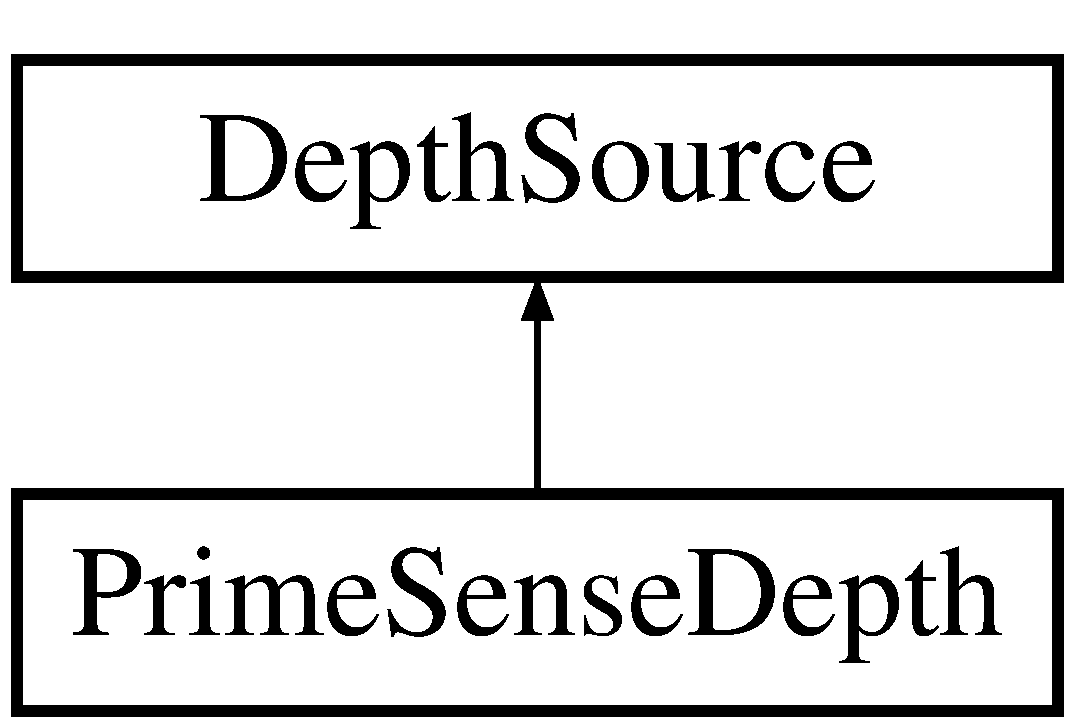
\includegraphics[height=2.000000cm]{classfovis_1_1PrimeSenseDepth}
\end{center}
\end{figure}
\subsection*{Public Member Functions}
\begin{DoxyCompactItemize}
\item 
double \hyperlink{classfovis_1_1PrimeSenseDepth_a1941b0a011e836e922ce08cf48c635f9}{getBaseline} () const 
\item 
uint16\_\-t \hyperlink{classfovis_1_1PrimeSenseDepth_a2b700699b1150d1c3ce269eac01b897b}{getDisparity} (int rgb\_\-u, int rgb\_\-v) const 
\item 
uint16\_\-t \hyperlink{classfovis_1_1PrimeSenseDepth_a5e3469916e73c978f8ddabbbece456cf}{getDisparityAtIRPixel} (int ir\_\-u, int ir\_\-v) const 
\item 
void \hyperlink{classfovis_1_1PrimeSenseDepth_a9ba60dfd976745761bb861f08a374679}{getXyz} (\hyperlink{classfovis_1_1OdometryFrame}{OdometryFrame} $\ast$frame)
\item 
\hypertarget{classfovis_1_1PrimeSenseDepth_ae02d9ae398ad1009deb51c39ea4e7272}{
bool {\bfseries getXyz} (int u, int v, Eigen::Vector3d \&xyz)}
\label{classfovis_1_1PrimeSenseDepth_ae02d9ae398ad1009deb51c39ea4e7272}

\item 
bool \hyperlink{classfovis_1_1PrimeSenseDepth_af5915074d7b5e0694bcb0fae662c6c6c}{haveXyz} (int u, int v)
\item 
\hypertarget{classfovis_1_1PrimeSenseDepth_a31ff2c09c45447a349a0b628e15f66e9}{
{\bfseries PrimeSenseDepth} (const \hyperlink{classfovis_1_1PrimeSenseCalibration}{PrimeSenseCalibration} $\ast$calib)}
\label{classfovis_1_1PrimeSenseDepth_a31ff2c09c45447a349a0b628e15f66e9}

\item 
void \hyperlink{classfovis_1_1PrimeSenseDepth_a39e83560fd704306d53858d07d61621b}{refineXyz} (\hyperlink{classfovis_1_1FeatureMatch}{FeatureMatch} $\ast$matches, int num\_\-matches, \hyperlink{classfovis_1_1OdometryFrame}{OdometryFrame} $\ast$frame)
\item 
\hypertarget{classfovis_1_1PrimeSenseDepth_ac821e5da15e9dcb63fe49702d38c22ea}{
void {\bfseries setDisparityData} (const uint16\_\-t $\ast$disparity)}
\label{classfovis_1_1PrimeSenseDepth_ac821e5da15e9dcb63fe49702d38c22ea}

\end{DoxyCompactItemize}


\subsection{Detailed Description}
Stores depth data for a Kinect / PrimeSense camera. 

\begin{DoxySeeAlso}{See also}
\hyperlink{structfovis_1_1PrimeSenseCalibrationParameters}{PrimeSenseCalibrationParameters}, \hyperlink{classfovis_1_1PrimeSenseCalibration}{PrimeSenseCalibration} 
\end{DoxySeeAlso}


\subsection{Member Function Documentation}
\hypertarget{classfovis_1_1PrimeSenseDepth_a9ba60dfd976745761bb861f08a374679}{
\index{fovis::PrimeSenseDepth@{fovis::PrimeSenseDepth}!getXyz@{getXyz}}
\index{getXyz@{getXyz}!fovis::PrimeSenseDepth@{fovis::PrimeSenseDepth}}
\subsubsection[{getXyz}]{\setlength{\rightskip}{0pt plus 5cm}void getXyz (
\begin{DoxyParamCaption}
\item[{{\bf OdometryFrame} $\ast$}]{frame}
\end{DoxyParamCaption}
)\hspace{0.3cm}{\ttfamily  \mbox{[}virtual\mbox{]}}}}
\label{classfovis_1_1PrimeSenseDepth_a9ba60dfd976745761bb861f08a374679}
Populate keypoints in frame with XYZ data. 

Implements \hyperlink{classfovis_1_1DepthSource_a0259f77a02ba85f5370407db4759d16a}{DepthSource}.

\hypertarget{classfovis_1_1PrimeSenseDepth_a39e83560fd704306d53858d07d61621b}{
\index{fovis::PrimeSenseDepth@{fovis::PrimeSenseDepth}!refineXyz@{refineXyz}}
\index{refineXyz@{refineXyz}!fovis::PrimeSenseDepth@{fovis::PrimeSenseDepth}}
\subsubsection[{refineXyz}]{\setlength{\rightskip}{0pt plus 5cm}void refineXyz (
\begin{DoxyParamCaption}
\item[{{\bf FeatureMatch} $\ast$}]{matches, }
\item[{int}]{num\_\-matches, }
\item[{{\bf OdometryFrame} $\ast$}]{frame}
\end{DoxyParamCaption}
)\hspace{0.3cm}{\ttfamily  \mbox{[}virtual\mbox{]}}}}
\label{classfovis_1_1PrimeSenseDepth_a39e83560fd704306d53858d07d61621b}
Refine XYZ data of target keypoints in matches (usually after subpixel refinement of the matches across time). 

Implements \hyperlink{classfovis_1_1DepthSource_a4d6eafb84371d0720cd7ee53ac2e659a}{DepthSource}.

\hypertarget{classfovis_1_1PrimeSenseDepth_a2b700699b1150d1c3ce269eac01b897b}{
\index{fovis::PrimeSenseDepth@{fovis::PrimeSenseDepth}!getDisparity@{getDisparity}}
\index{getDisparity@{getDisparity}!fovis::PrimeSenseDepth@{fovis::PrimeSenseDepth}}
\subsubsection[{getDisparity}]{\setlength{\rightskip}{0pt plus 5cm}uint16\_\-t getDisparity (
\begin{DoxyParamCaption}
\item[{int}]{rgb\_\-u, }
\item[{int}]{rgb\_\-v}
\end{DoxyParamCaption}
) const\hspace{0.3cm}{\ttfamily  \mbox{[}inline\mbox{]}}}}
\label{classfovis_1_1PrimeSenseDepth_a2b700699b1150d1c3ce269eac01b897b}
Retrieve the disparity value at the IR pixel that projects on to the specified RGB pixel.

Disparity is not measured on the RGB image directly. Instead, it's measured on the IR image, then the points are projected onto the RGB image. This function looks up the IR pixel that projected onto the specified RGB pixel, and then returns the disparity of the IR pixel.

Returns: the measured disparity, or 0 if there is no disparity data for the specified pixel. \hypertarget{classfovis_1_1PrimeSenseDepth_a5e3469916e73c978f8ddabbbece456cf}{
\index{fovis::PrimeSenseDepth@{fovis::PrimeSenseDepth}!getDisparityAtIRPixel@{getDisparityAtIRPixel}}
\index{getDisparityAtIRPixel@{getDisparityAtIRPixel}!fovis::PrimeSenseDepth@{fovis::PrimeSenseDepth}}
\subsubsection[{getDisparityAtIRPixel}]{\setlength{\rightskip}{0pt plus 5cm}uint16\_\-t getDisparityAtIRPixel (
\begin{DoxyParamCaption}
\item[{int}]{ir\_\-u, }
\item[{int}]{ir\_\-v}
\end{DoxyParamCaption}
) const\hspace{0.3cm}{\ttfamily  \mbox{[}inline\mbox{]}}}}
\label{classfovis_1_1PrimeSenseDepth_a5e3469916e73c978f8ddabbbece456cf}
Retrieve the disparity value at the specified RGB pixel. \hypertarget{classfovis_1_1PrimeSenseDepth_a1941b0a011e836e922ce08cf48c635f9}{
\index{fovis::PrimeSenseDepth@{fovis::PrimeSenseDepth}!getBaseline@{getBaseline}}
\index{getBaseline@{getBaseline}!fovis::PrimeSenseDepth@{fovis::PrimeSenseDepth}}
\subsubsection[{getBaseline}]{\setlength{\rightskip}{0pt plus 5cm}double getBaseline (
\begin{DoxyParamCaption}
{}
\end{DoxyParamCaption}
) const\hspace{0.3cm}{\ttfamily  \mbox{[}inline, virtual\mbox{]}}}}
\label{classfovis_1_1PrimeSenseDepth_a1941b0a011e836e922ce08cf48c635f9}
Return baseline of depth source, if applicable. If not applicable (e.g. for OpenNI devices) return 0. 

Implements \hyperlink{classfovis_1_1DepthSource_a22d76295f183f3ec9e34d2d7e837c675}{DepthSource}.

\hypertarget{classfovis_1_1PrimeSenseDepth_af5915074d7b5e0694bcb0fae662c6c6c}{
\index{fovis::PrimeSenseDepth@{fovis::PrimeSenseDepth}!haveXyz@{haveXyz}}
\index{haveXyz@{haveXyz}!fovis::PrimeSenseDepth@{fovis::PrimeSenseDepth}}
\subsubsection[{haveXyz}]{\setlength{\rightskip}{0pt plus 5cm}bool haveXyz (
\begin{DoxyParamCaption}
\item[{int}]{u, }
\item[{int}]{v}
\end{DoxyParamCaption}
)\hspace{0.3cm}{\ttfamily  \mbox{[}inline, virtual\mbox{]}}}}
\label{classfovis_1_1PrimeSenseDepth_af5915074d7b5e0694bcb0fae662c6c6c}
This should return true if it's not certain there's no depth at (u,v). It should be an inexpensive check that is used to avoid pointless (hah!) creation of keypoints. False positives are fine as ling as getXyz gets rid of them. 

Implements \hyperlink{classfovis_1_1DepthSource_ad0d2b9dd0e48e428319c3c84e87fa5cf}{DepthSource}.



The documentation for this class was generated from the following file:\begin{DoxyCompactItemize}
\item 
primesense\_\-depth.hpp\end{DoxyCompactItemize}

\hypertarget{classfovis_1_1PyramidLevel}{
\section{PyramidLevel Class Reference}
\label{classfovis_1_1PyramidLevel}\index{fovis::PyramidLevel@{fovis::PyramidLevel}}
}


One level of a Gaussian image pyramid.  


\subsection*{Public Member Functions}
\begin{DoxyCompactItemize}
\item 
\hypertarget{classfovis_1_1PyramidLevel_af18feed592ad68f72aaee04c31021932}{
const uint8\_\-t $\ast$ {\bfseries getDescriptor} (int i) const }
\label{classfovis_1_1PyramidLevel_af18feed592ad68f72aaee04c31021932}

\item 
\hypertarget{classfovis_1_1PyramidLevel_acb4a60e9159801a3486dd6f2081cf346}{
const int $\ast$ {\bfseries getDescriptorIndexOffsets} () const }
\label{classfovis_1_1PyramidLevel_acb4a60e9159801a3486dd6f2081cf346}

\item 
\hypertarget{classfovis_1_1PyramidLevel_ace19c8012ae7eaa4db2f807167b165f9}{
int {\bfseries getDescriptorLength} () const }
\label{classfovis_1_1PyramidLevel_ace19c8012ae7eaa4db2f807167b165f9}

\item 
\hypertarget{classfovis_1_1PyramidLevel_ab19595fa4e4bb6716f9ed7fa38a297b2}{
int {\bfseries getDescriptorStride} () const }
\label{classfovis_1_1PyramidLevel_ab19595fa4e4bb6716f9ed7fa38a297b2}

\item 
\hypertarget{classfovis_1_1PyramidLevel_a5ecca567fb6513c431d45af12bb21e96}{
const uint8\_\-t $\ast$ {\bfseries getGrayscaleImage} () const }
\label{classfovis_1_1PyramidLevel_a5ecca567fb6513c431d45af12bb21e96}

\item 
\hypertarget{classfovis_1_1PyramidLevel_a88777237ef606ffe6653a0f7eda10bd5}{
int {\bfseries getGrayscaleImageStride} () const }
\label{classfovis_1_1PyramidLevel_a88777237ef606ffe6653a0f7eda10bd5}

\item 
\hypertarget{classfovis_1_1PyramidLevel_a317329daf960a1759801c0f16d43d5a3}{
int {\bfseries getHeight} () const }
\label{classfovis_1_1PyramidLevel_a317329daf960a1759801c0f16d43d5a3}

\item 
\hypertarget{classfovis_1_1PyramidLevel_a862d98fc6ffbe2d9e9eefa96a5204f82}{
const std::vector$<$ \hyperlink{classfovis_1_1KeyPoint}{KeyPoint} $>$ \& {\bfseries getInitialFeatures} () const }
\label{classfovis_1_1PyramidLevel_a862d98fc6ffbe2d9e9eefa96a5204f82}

\item 
\hypertarget{classfovis_1_1PyramidLevel_ac76712b2fb8617f6b40cfd7b52a4578c}{
const \hyperlink{classfovis_1_1KeyPoint}{KeyPoint} \& {\bfseries getKeypoint} (int i) const }
\label{classfovis_1_1PyramidLevel_ac76712b2fb8617f6b40cfd7b52a4578c}

\item 
\hypertarget{classfovis_1_1PyramidLevel_ae384c7beac17bdc5a66f7e0b09371a4f}{
const \hyperlink{classfovis_1_1KeypointData}{KeypointData} $\ast$ {\bfseries getKeypointData} (int i) const }
\label{classfovis_1_1PyramidLevel_ae384c7beac17bdc5a66f7e0b09371a4f}

\item 
\hypertarget{classfovis_1_1PyramidLevel_a10ac8acd277ef2a168162489fe8dab8b}{
\hyperlink{classfovis_1_1KeypointData}{KeypointData} $\ast$ {\bfseries getKeypointData} (int i)}
\label{classfovis_1_1PyramidLevel_a10ac8acd277ef2a168162489fe8dab8b}

\item 
\hypertarget{classfovis_1_1PyramidLevel_af35b57abfc0059c951e3f9acc0dfb756}{
const float {\bfseries getKeypointRectBaseU} (int kp\_\-index) const }
\label{classfovis_1_1PyramidLevel_af35b57abfc0059c951e3f9acc0dfb756}

\item 
\hypertarget{classfovis_1_1PyramidLevel_a4bd19b62564e3e74453a551539c72397}{
const Eigen::Vector2d \& {\bfseries getKeypointRectBaseUV} (int kp\_\-index) const }
\label{classfovis_1_1PyramidLevel_a4bd19b62564e3e74453a551539c72397}

\item 
\hypertarget{classfovis_1_1PyramidLevel_a7ea0d7902de164ffd9817b0274901c57}{
const float {\bfseries getKeypointRectBaseV} (int kp\_\-index) const }
\label{classfovis_1_1PyramidLevel_a7ea0d7902de164ffd9817b0274901c57}

\item 
\hypertarget{classfovis_1_1PyramidLevel_a954f048408c43362b316cc202142b9f4}{
const Eigen::Vector4d \& {\bfseries getKeypointXYZW} (int i) const }
\label{classfovis_1_1PyramidLevel_a954f048408c43362b316cc202142b9f4}

\item 
\hypertarget{classfovis_1_1PyramidLevel_ad4dc7171634839f3dedc2e90a2d6ef33}{
int {\bfseries getLevelNum} () const }
\label{classfovis_1_1PyramidLevel_ad4dc7171634839f3dedc2e90a2d6ef33}

\item 
\hypertarget{classfovis_1_1PyramidLevel_a6b34494d5f8a1666d216bae16f25640b}{
int {\bfseries getNumDetectedKeypoints} () const }
\label{classfovis_1_1PyramidLevel_a6b34494d5f8a1666d216bae16f25640b}

\item 
\hypertarget{classfovis_1_1PyramidLevel_ac411e38b8e5d28686355d6e7afece27f}{
int {\bfseries getNumKeypoints} () const }
\label{classfovis_1_1PyramidLevel_ac411e38b8e5d28686355d6e7afece27f}

\item 
\hypertarget{classfovis_1_1PyramidLevel_af149cb053bc8b5fbc1364b5dbb934488}{
int {\bfseries getWidth} () const }
\label{classfovis_1_1PyramidLevel_af149cb053bc8b5fbc1364b5dbb934488}

\item 
\hypertarget{classfovis_1_1PyramidLevel_a3a4ff5f0cd0c0b72661126fc123d8838}{
bool {\bfseries isLegalKeypointCoordinate} (float x, float y) const }
\label{classfovis_1_1PyramidLevel_a3a4ff5f0cd0c0b72661126fc123d8838}

\item 
\hypertarget{classfovis_1_1PyramidLevel_af4ea0dd228424433c9427082b2e7b6bc}{
void {\bfseries populateDescriptorAligned} (int x, int y, uint8\_\-t $\ast$descriptor) const }
\label{classfovis_1_1PyramidLevel_af4ea0dd228424433c9427082b2e7b6bc}

\item 
\hypertarget{classfovis_1_1PyramidLevel_a09ba1facc91001f282aa0e6773154e97}{
void {\bfseries populateDescriptorInterp} (float x, float y, uint8\_\-t $\ast$descriptor) const }
\label{classfovis_1_1PyramidLevel_a09ba1facc91001f282aa0e6773154e97}

\item 
\hypertarget{classfovis_1_1PyramidLevel_a525d0403c51c51b9548b05b83ac8fb37}{
void {\bfseries populateDescriptorsAligned} (const \hyperlink{classfovis_1_1KeypointData}{KeypointData} $\ast$keypoints, int num\_\-keypoints, uint8\_\-t $\ast$descriptors) const }
\label{classfovis_1_1PyramidLevel_a525d0403c51c51b9548b05b83ac8fb37}

\item 
\hypertarget{classfovis_1_1PyramidLevel_a686da131ed7363eb73ec6643e25d0d27}{
void {\bfseries populateDescriptorsInterp} (const \hyperlink{classfovis_1_1KeypointData}{KeypointData} $\ast$keypoints, int num\_\-keypoints, uint8\_\-t $\ast$descriptors) const }
\label{classfovis_1_1PyramidLevel_a686da131ed7363eb73ec6643e25d0d27}

\item 
\hypertarget{classfovis_1_1PyramidLevel_a1d7e0bd5a1376e477d5f574783b4620f}{
{\bfseries PyramidLevel} (int width, int height, int level\_\-num, int feature\_\-window\_\-size, \hyperlink{classfovis_1_1GridKeyPointFilter}{GridKeyPointFilter} \&grid\_\-filter)}
\label{classfovis_1_1PyramidLevel_a1d7e0bd5a1376e477d5f574783b4620f}

\end{DoxyCompactItemize}
\subsection*{Friends}
\begin{DoxyCompactItemize}
\item 
\hypertarget{classfovis_1_1PyramidLevel_a50334ce695e3432bfd1bf2210c64f696}{
class {\bfseries OdometryFrame}}
\label{classfovis_1_1PyramidLevel_a50334ce695e3432bfd1bf2210c64f696}

\item 
\hypertarget{classfovis_1_1PyramidLevel_a1b97353efc48811a6a200c07b99c74e6}{
class {\bfseries StereoFrame}}
\label{classfovis_1_1PyramidLevel_a1b97353efc48811a6a200c07b99c74e6}

\end{DoxyCompactItemize}


\subsection{Detailed Description}
One level of a Gaussian image pyramid. 

TODO 

The documentation for this class was generated from the following file:\begin{DoxyCompactItemize}
\item 
pyramid\_\-level.hpp\end{DoxyCompactItemize}

\hypertarget{classfovis_1_1Rectification}{
\section{Rectification Class Reference}
\label{classfovis_1_1Rectification}\index{fovis::Rectification@{fovis::Rectification}}
}


Maps image coordinates from an input image to image coordinates on a rectified camera.  


\subsection*{Public Member Functions}
\begin{DoxyCompactItemize}
\item 
const \hyperlink{structfovis_1_1CameraIntrinsicsParameters}{CameraIntrinsicsParameters} \& \hyperlink{classfovis_1_1Rectification_a26b289f3a9422898e0827833500f5a7f}{getInputCameraParameters} () const 
\item 
const Eigen::Matrix3d \& \hyperlink{classfovis_1_1Rectification_aad9df4b38b1c567ab56c3fceb1f51193}{getRectificationRotation} () const 
\item 
const \hyperlink{structfovis_1_1CameraIntrinsicsParameters}{CameraIntrinsicsParameters} \& \hyperlink{classfovis_1_1Rectification_ac3e99685d2431ad016434b13edf5a7e0}{getRectifiedCameraParameters} () const 
\item 
\hyperlink{classfovis_1_1Rectification}{Rectification} $\ast$ \hyperlink{classfovis_1_1Rectification_acd7ab855a169e8260203e83dc926e31c}{makeCopy} () const 
\item 
\hyperlink{classfovis_1_1Rectification_a850b5be87e72670261ef158a13a02606}{Rectification} (const \hyperlink{structfovis_1_1CameraIntrinsicsParameters}{CameraIntrinsicsParameters} \&input\_\-camera\_\-params, const Eigen::Matrix3d \&rotation, const \hyperlink{structfovis_1_1CameraIntrinsicsParameters}{CameraIntrinsicsParameters} \&rectified\_\-camera\_\-params)
\item 
\hyperlink{classfovis_1_1Rectification_a63a08ffa2c5fd3bf905f0a2949a14178}{Rectification} (const \hyperlink{structfovis_1_1CameraIntrinsicsParameters}{CameraIntrinsicsParameters} \&input\_\-camera\_\-params)
\item 
void \hyperlink{classfovis_1_1Rectification_a6ede2d21c8bfe048f16ec510e53bd7c7}{rectifyBilinearLookup} (const Eigen::Vector2d \&dist\_\-uv, Eigen::Vector2d $\ast$rect\_\-uv) const 
\item 
void \hyperlink{classfovis_1_1Rectification_a997ec4bb4cf597491445a8e42e183e5d}{rectifyLookup} (int dist\_\-u, int dist\_\-v, Eigen::Vector2d $\ast$rect\_\-uv) const 
\item 
void \hyperlink{classfovis_1_1Rectification_ac898654ec6adbc843e8e036736ae077f}{rectifyLookupByIndex} (int pixel\_\-index, Eigen::Vector2d $\ast$rect\_\-uv) const 
\end{DoxyCompactItemize}


\subsection{Detailed Description}
Maps image coordinates from an input image to image coordinates on a rectified camera. 

A \hyperlink{classfovis_1_1Rectification}{Rectification} object represents the computation required to map pixels from an input camera to pixels on a \char`\"{}rectified\char`\"{} virtual camera that shares the same focal point, but may be rotated and have different projection parameters (e.g., focal length, center of projection, etc.)

This class is primary useful with stereo cameras to rectify pixels on both input cameras to rectified cameras that share an image plane and look/up vectors. It can also be used for simple undistortion (e.g., no rotation, and a rectified camera that has the same projection parameters as the input camera, but with no distortion).

For fast rectification, the \hyperlink{classfovis_1_1Rectification}{Rectification} object precomputes a mapping from (u, v) image pixel coordinates to u', v' rectified image pixel coordinates. The exact transformation from (u, v) to (u', v') is:


\begin{DoxyEnumerate}
\item undistort according to a plumb-\/bob distortion model
\item rotate points about the origin
\item reproject onto a rectified image plane.
\end{DoxyEnumerate}

\hyperlink{classfovis_1_1Rectification}{Rectification} of pixels is done by bilinear interpolation on this precomputed mapping. 

\subsection{Constructor \& Destructor Documentation}
\hypertarget{classfovis_1_1Rectification_a63a08ffa2c5fd3bf905f0a2949a14178}{
\index{fovis::Rectification@{fovis::Rectification}!Rectification@{Rectification}}
\index{Rectification@{Rectification}!fovis::Rectification@{fovis::Rectification}}
\subsubsection[{Rectification}]{\setlength{\rightskip}{0pt plus 5cm}{\bf Rectification} (
\begin{DoxyParamCaption}
\item[{const {\bf CameraIntrinsicsParameters} \&}]{input\_\-camera\_\-params}
\end{DoxyParamCaption}
)}}
\label{classfovis_1_1Rectification_a63a08ffa2c5fd3bf905f0a2949a14178}
Convenience constructor to create a \hyperlink{classfovis_1_1Rectification}{Rectification} object that simply undistorts. The rotation is set to identity, and the rectified camera parameters are identical to the input camera parameters, but have no distortion. \hypertarget{classfovis_1_1Rectification_a850b5be87e72670261ef158a13a02606}{
\index{fovis::Rectification@{fovis::Rectification}!Rectification@{Rectification}}
\index{Rectification@{Rectification}!fovis::Rectification@{fovis::Rectification}}
\subsubsection[{Rectification}]{\setlength{\rightskip}{0pt plus 5cm}{\bf Rectification} (
\begin{DoxyParamCaption}
\item[{const {\bf CameraIntrinsicsParameters} \&}]{input\_\-camera\_\-params, }
\item[{const Eigen::Matrix3d \&}]{rotation, }
\item[{const {\bf CameraIntrinsicsParameters} \&}]{rectified\_\-camera\_\-params}
\end{DoxyParamCaption}
)}}
\label{classfovis_1_1Rectification_a850b5be87e72670261ef158a13a02606}
Constructor. The rectified\_\-camera\_\-params are not allowed to have any distortion. 

\subsection{Member Function Documentation}
\hypertarget{classfovis_1_1Rectification_a26b289f3a9422898e0827833500f5a7f}{
\index{fovis::Rectification@{fovis::Rectification}!getInputCameraParameters@{getInputCameraParameters}}
\index{getInputCameraParameters@{getInputCameraParameters}!fovis::Rectification@{fovis::Rectification}}
\subsubsection[{getInputCameraParameters}]{\setlength{\rightskip}{0pt plus 5cm}const {\bf CameraIntrinsicsParameters}\& getInputCameraParameters (
\begin{DoxyParamCaption}
{}
\end{DoxyParamCaption}
) const\hspace{0.3cm}{\ttfamily  \mbox{[}inline\mbox{]}}}}
\label{classfovis_1_1Rectification_a26b289f3a9422898e0827833500f5a7f}
\begin{DoxyReturn}{Returns}
the intrisic parameters of the input camera. 
\end{DoxyReturn}
\hypertarget{classfovis_1_1Rectification_aad9df4b38b1c567ab56c3fceb1f51193}{
\index{fovis::Rectification@{fovis::Rectification}!getRectificationRotation@{getRectificationRotation}}
\index{getRectificationRotation@{getRectificationRotation}!fovis::Rectification@{fovis::Rectification}}
\subsubsection[{getRectificationRotation}]{\setlength{\rightskip}{0pt plus 5cm}const Eigen::Matrix3d\& getRectificationRotation (
\begin{DoxyParamCaption}
{}
\end{DoxyParamCaption}
) const\hspace{0.3cm}{\ttfamily  \mbox{[}inline\mbox{]}}}}
\label{classfovis_1_1Rectification_aad9df4b38b1c567ab56c3fceb1f51193}
\begin{DoxyReturn}{Returns}
the rotation to apply between the undistorted input camera frame and the output rectified camera frame. 
\end{DoxyReturn}
\hypertarget{classfovis_1_1Rectification_ac3e99685d2431ad016434b13edf5a7e0}{
\index{fovis::Rectification@{fovis::Rectification}!getRectifiedCameraParameters@{getRectifiedCameraParameters}}
\index{getRectifiedCameraParameters@{getRectifiedCameraParameters}!fovis::Rectification@{fovis::Rectification}}
\subsubsection[{getRectifiedCameraParameters}]{\setlength{\rightskip}{0pt plus 5cm}const {\bf CameraIntrinsicsParameters}\& getRectifiedCameraParameters (
\begin{DoxyParamCaption}
{}
\end{DoxyParamCaption}
) const\hspace{0.3cm}{\ttfamily  \mbox{[}inline\mbox{]}}}}
\label{classfovis_1_1Rectification_ac3e99685d2431ad016434b13edf5a7e0}
\begin{DoxyReturn}{Returns}
the projection parameters of the rectified camera. The distortion coefficients will always be zero. Note that the focal length and image dimensions of the rectified camera do not have to match those of the input camera. 
\end{DoxyReturn}
\hypertarget{classfovis_1_1Rectification_a997ec4bb4cf597491445a8e42e183e5d}{
\index{fovis::Rectification@{fovis::Rectification}!rectifyLookup@{rectifyLookup}}
\index{rectifyLookup@{rectifyLookup}!fovis::Rectification@{fovis::Rectification}}
\subsubsection[{rectifyLookup}]{\setlength{\rightskip}{0pt plus 5cm}void rectifyLookup (
\begin{DoxyParamCaption}
\item[{int}]{dist\_\-u, }
\item[{int}]{dist\_\-v, }
\item[{Eigen::Vector2d $\ast$}]{rect\_\-uv}
\end{DoxyParamCaption}
) const\hspace{0.3cm}{\ttfamily  \mbox{[}inline\mbox{]}}}}
\label{classfovis_1_1Rectification_a997ec4bb4cf597491445a8e42e183e5d}
Computes the undistorted image coordinates of the input distorted coordinates ({\ttfamily dist\_\-u}, {\ttfamily dist\_\-v}).


\begin{DoxyParams}{Parameters}
{\em dist\_\-u} & input distorted pixel u/x coordinate. \\
\hline
{\em dist\_\-v} & input distorted pixel v/y coordinate. \\
\hline
{\em rect\_\-uv} & output parameter. \\
\hline
\end{DoxyParams}
\hypertarget{classfovis_1_1Rectification_ac898654ec6adbc843e8e036736ae077f}{
\index{fovis::Rectification@{fovis::Rectification}!rectifyLookupByIndex@{rectifyLookupByIndex}}
\index{rectifyLookupByIndex@{rectifyLookupByIndex}!fovis::Rectification@{fovis::Rectification}}
\subsubsection[{rectifyLookupByIndex}]{\setlength{\rightskip}{0pt plus 5cm}void rectifyLookupByIndex (
\begin{DoxyParamCaption}
\item[{int}]{pixel\_\-index, }
\item[{Eigen::Vector2d $\ast$}]{rect\_\-uv}
\end{DoxyParamCaption}
) const\hspace{0.3cm}{\ttfamily  \mbox{[}inline\mbox{]}}}}
\label{classfovis_1_1Rectification_ac898654ec6adbc843e8e036736ae077f}
Computes the undistorted image coordinates of an input pixel specified by its row-\/major pixel index.


\begin{DoxyParams}{Parameters}
{\em pixel\_\-index} & corresponds to $ u * width + v $ \\
\hline
{\em rect\_\-uv} & output parameter.\\
\hline
\end{DoxyParams}
\begin{DoxySeeAlso}{See also}
\hyperlink{classfovis_1_1Rectification_a997ec4bb4cf597491445a8e42e183e5d}{rectifyLookup} 
\end{DoxySeeAlso}
\hypertarget{classfovis_1_1Rectification_a6ede2d21c8bfe048f16ec510e53bd7c7}{
\index{fovis::Rectification@{fovis::Rectification}!rectifyBilinearLookup@{rectifyBilinearLookup}}
\index{rectifyBilinearLookup@{rectifyBilinearLookup}!fovis::Rectification@{fovis::Rectification}}
\subsubsection[{rectifyBilinearLookup}]{\setlength{\rightskip}{0pt plus 5cm}void rectifyBilinearLookup (
\begin{DoxyParamCaption}
\item[{const Eigen::Vector2d \&}]{dist\_\-uv, }
\item[{Eigen::Vector2d $\ast$}]{rect\_\-uv}
\end{DoxyParamCaption}
) const\hspace{0.3cm}{\ttfamily  \mbox{[}inline\mbox{]}}}}
\label{classfovis_1_1Rectification_a6ede2d21c8bfe048f16ec510e53bd7c7}
Computes the undistorted image coordinates of an input pixel via bilinear interpolation of its integer-\/coordinate 4-\/neighboors.


\begin{DoxyParams}{Parameters}
{\em dist\_\-uv} & input distorted pixel coordinates. \\
\hline
{\em rect\_\-uv} & output parameter. \\
\hline
\end{DoxyParams}
\hypertarget{classfovis_1_1Rectification_acd7ab855a169e8260203e83dc926e31c}{
\index{fovis::Rectification@{fovis::Rectification}!makeCopy@{makeCopy}}
\index{makeCopy@{makeCopy}!fovis::Rectification@{fovis::Rectification}}
\subsubsection[{makeCopy}]{\setlength{\rightskip}{0pt plus 5cm}{\bf Rectification}$\ast$ makeCopy (
\begin{DoxyParamCaption}
{}
\end{DoxyParamCaption}
) const}}
\label{classfovis_1_1Rectification_acd7ab855a169e8260203e83dc926e31c}
\begin{DoxyReturn}{Returns}
a deep copy of this object. 
\end{DoxyReturn}


The documentation for this class was generated from the following file:\begin{DoxyCompactItemize}
\item 
rectification.hpp\end{DoxyCompactItemize}

\hypertarget{classfovis_1_1SAD}{
\section{SAD Class Reference}
\label{classfovis_1_1SAD}\index{fovis::SAD@{fovis::SAD}}
}


Calculates the Sum of Absolute Deviations (\hyperlink{classfovis_1_1SAD}{SAD}) score between two vectors of length descriptor\_\-len.  


\subsection*{Public Member Functions}
\begin{DoxyCompactItemize}
\item 
\hypertarget{classfovis_1_1SAD_a9ce8d3af51f97c40bac28d95bb550493}{
int {\bfseries getWorstScore} () const }
\label{classfovis_1_1SAD_a9ce8d3af51f97c40bac28d95bb550493}

\item 
\hypertarget{classfovis_1_1SAD_ac2a3cf5966a597da6e9101e25c7d87f0}{
{\bfseries SAD} (int descriptor\_\-len)}
\label{classfovis_1_1SAD_ac2a3cf5966a597da6e9101e25c7d87f0}

\item 
int32\_\-t \hyperlink{classfovis_1_1SAD_a28e42afefdce36393367c8748d11f265}{score} (const uint8\_\-t $\ast$ref\_\-desc, const uint8\_\-t $\ast$target\_\-desc)
\end{DoxyCompactItemize}


\subsection{Detailed Description}
Calculates the Sum of Absolute Deviations (\hyperlink{classfovis_1_1SAD}{SAD}) score between two vectors of length descriptor\_\-len. 

\subsection{Member Function Documentation}
\hypertarget{classfovis_1_1SAD_a28e42afefdce36393367c8748d11f265}{
\index{fovis::SAD@{fovis::SAD}!score@{score}}
\index{score@{score}!fovis::SAD@{fovis::SAD}}
\subsubsection[{score}]{\setlength{\rightskip}{0pt plus 5cm}int32\_\-t score (
\begin{DoxyParamCaption}
\item[{const uint8\_\-t $\ast$}]{ref\_\-desc, }
\item[{const uint8\_\-t $\ast$}]{target\_\-desc}
\end{DoxyParamCaption}
)\hspace{0.3cm}{\ttfamily  \mbox{[}inline\mbox{]}}}}
\label{classfovis_1_1SAD_a28e42afefdce36393367c8748d11f265}
Calculate \hyperlink{classfovis_1_1SAD}{SAD} score between ref\_\-desc and target\_\-desc. ref\_\-desc and target\_\-desc must be padded with zero-\/filled pad bytes up to multiple of 16. 

The documentation for this class was generated from the following file:\begin{DoxyCompactItemize}
\item 
sad.hpp\end{DoxyCompactItemize}

\hypertarget{classfovis_1_1StereoCalibration}{
\section{StereoCalibration Class Reference}
\label{classfovis_1_1StereoCalibration}\index{fovis::StereoCalibration@{fovis::StereoCalibration}}
}


Computes useful information from a \hyperlink{structfovis_1_1StereoCalibrationParameters}{StereoCalibrationParameters} object.  


\subsection*{Public Member Functions}
\begin{DoxyCompactItemize}
\item 
\hypertarget{classfovis_1_1StereoCalibration_a1941b0a011e836e922ce08cf48c635f9}{
double {\bfseries getBaseline} () const }
\label{classfovis_1_1StereoCalibration_a1941b0a011e836e922ce08cf48c635f9}

\item 
int \hyperlink{classfovis_1_1StereoCalibration_a317329daf960a1759801c0f16d43d5a3}{getHeight} () const 
\item 
\hypertarget{classfovis_1_1StereoCalibration_a536e3a1c9ce494e4aa7fd26b6052dcdf}{
const \hyperlink{classfovis_1_1Rectification}{Rectification} $\ast$ {\bfseries getLeftRectification} () const }
\label{classfovis_1_1StereoCalibration_a536e3a1c9ce494e4aa7fd26b6052dcdf}

\item 
\hypertarget{classfovis_1_1StereoCalibration_ab2d2a83222ec0129d145428e46ef3402}{
const \hyperlink{structfovis_1_1CameraIntrinsicsParameters}{CameraIntrinsicsParameters} \& {\bfseries getRectifiedParameters} () const }
\label{classfovis_1_1StereoCalibration_ab2d2a83222ec0129d145428e46ef3402}

\item 
\hypertarget{classfovis_1_1StereoCalibration_a20ce4a3aaa724f8cf89da6d3c7fc9a6a}{
const \hyperlink{classfovis_1_1Rectification}{Rectification} $\ast$ {\bfseries getRightRectification} () const }
\label{classfovis_1_1StereoCalibration_a20ce4a3aaa724f8cf89da6d3c7fc9a6a}

\item 
Eigen::Matrix4d \hyperlink{classfovis_1_1StereoCalibration_a1719db5b17bd3d44657bad9a41000696}{getUvdToXyz} () const 
\item 
int \hyperlink{classfovis_1_1StereoCalibration_af149cb053bc8b5fbc1364b5dbb934488}{getWidth} () const 
\item 
\hyperlink{classfovis_1_1StereoCalibration}{StereoCalibration} $\ast$ \hyperlink{classfovis_1_1StereoCalibration_ac9cd053e6a872120501d02a8380ae7f5}{makeCopy} () const 
\item 
\hypertarget{classfovis_1_1StereoCalibration_a458a750c764033004d225eb12061784d}{
{\bfseries StereoCalibration} (const \hyperlink{structfovis_1_1StereoCalibrationParameters}{StereoCalibrationParameters} \&params)}
\label{classfovis_1_1StereoCalibration_a458a750c764033004d225eb12061784d}

\end{DoxyCompactItemize}


\subsection{Detailed Description}
Computes useful information from a \hyperlink{structfovis_1_1StereoCalibrationParameters}{StereoCalibrationParameters} object. 

\subsection{Member Function Documentation}
\hypertarget{classfovis_1_1StereoCalibration_a1719db5b17bd3d44657bad9a41000696}{
\index{fovis::StereoCalibration@{fovis::StereoCalibration}!getUvdToXyz@{getUvdToXyz}}
\index{getUvdToXyz@{getUvdToXyz}!fovis::StereoCalibration@{fovis::StereoCalibration}}
\subsubsection[{getUvdToXyz}]{\setlength{\rightskip}{0pt plus 5cm}Eigen::Matrix4d getUvdToXyz (
\begin{DoxyParamCaption}
{}
\end{DoxyParamCaption}
) const\hspace{0.3cm}{\ttfamily  \mbox{[}inline\mbox{]}}}}
\label{classfovis_1_1StereoCalibration_a1719db5b17bd3d44657bad9a41000696}
Compute the 4x4 transformation matrix mapping \mbox{[} u, v, disparity, 1 \mbox{]} coordinates to \mbox{[} x, y, z, w \mbox{]} homogeneous coordinates in camera space. \hypertarget{classfovis_1_1StereoCalibration_af149cb053bc8b5fbc1364b5dbb934488}{
\index{fovis::StereoCalibration@{fovis::StereoCalibration}!getWidth@{getWidth}}
\index{getWidth@{getWidth}!fovis::StereoCalibration@{fovis::StereoCalibration}}
\subsubsection[{getWidth}]{\setlength{\rightskip}{0pt plus 5cm}int getWidth (
\begin{DoxyParamCaption}
{}
\end{DoxyParamCaption}
) const\hspace{0.3cm}{\ttfamily  \mbox{[}inline\mbox{]}}}}
\label{classfovis_1_1StereoCalibration_af149cb053bc8b5fbc1364b5dbb934488}
\begin{DoxyReturn}{Returns}
the width of the rectified camera. 
\end{DoxyReturn}
\hypertarget{classfovis_1_1StereoCalibration_a317329daf960a1759801c0f16d43d5a3}{
\index{fovis::StereoCalibration@{fovis::StereoCalibration}!getHeight@{getHeight}}
\index{getHeight@{getHeight}!fovis::StereoCalibration@{fovis::StereoCalibration}}
\subsubsection[{getHeight}]{\setlength{\rightskip}{0pt plus 5cm}int getHeight (
\begin{DoxyParamCaption}
{}
\end{DoxyParamCaption}
) const\hspace{0.3cm}{\ttfamily  \mbox{[}inline\mbox{]}}}}
\label{classfovis_1_1StereoCalibration_a317329daf960a1759801c0f16d43d5a3}
\begin{DoxyReturn}{Returns}
the height of the rectified camera. 
\end{DoxyReturn}
\hypertarget{classfovis_1_1StereoCalibration_ac9cd053e6a872120501d02a8380ae7f5}{
\index{fovis::StereoCalibration@{fovis::StereoCalibration}!makeCopy@{makeCopy}}
\index{makeCopy@{makeCopy}!fovis::StereoCalibration@{fovis::StereoCalibration}}
\subsubsection[{makeCopy}]{\setlength{\rightskip}{0pt plus 5cm}{\bf StereoCalibration}$\ast$ makeCopy (
\begin{DoxyParamCaption}
{}
\end{DoxyParamCaption}
) const}}
\label{classfovis_1_1StereoCalibration_ac9cd053e6a872120501d02a8380ae7f5}
\begin{DoxyReturn}{Returns}
a newly allocated copy of this calibration object. 
\end{DoxyReturn}


The documentation for this class was generated from the following file:\begin{DoxyCompactItemize}
\item 
stereo\_\-depth.hpp\end{DoxyCompactItemize}

\hypertarget{structfovis_1_1StereoCalibrationParameters}{
\section{StereoCalibrationParameters Struct Reference}
\label{structfovis_1_1StereoCalibrationParameters}\index{fovis::StereoCalibrationParameters@{fovis::StereoCalibrationParameters}}
}


Calibration data structure for stereo cameras.  


\subsection*{Public Attributes}
\begin{DoxyCompactItemize}
\item 
\hyperlink{structfovis_1_1CameraIntrinsicsParameters}{CameraIntrinsicsParameters} \hyperlink{structfovis_1_1StereoCalibrationParameters_ae2daad4ea93156558a55f3fa9a9d26e4}{left\_\-parameters}
\item 
\hyperlink{structfovis_1_1CameraIntrinsicsParameters}{CameraIntrinsicsParameters} \hyperlink{structfovis_1_1StereoCalibrationParameters_a873ffca7c3cd68f861b010bc7843e219}{right\_\-parameters}
\item 
double \hyperlink{structfovis_1_1StereoCalibrationParameters_ab3132502bb9c8258759a94659881e80c}{right\_\-to\_\-left\_\-rotation} \mbox{[}4\mbox{]}
\item 
double \hyperlink{structfovis_1_1StereoCalibrationParameters_adc32536cfff16a5a429ee922055e91c7}{right\_\-to\_\-left\_\-translation} \mbox{[}3\mbox{]}
\end{DoxyCompactItemize}


\subsection{Detailed Description}
Calibration data structure for stereo cameras. 

\subsection{Member Data Documentation}
\hypertarget{structfovis_1_1StereoCalibrationParameters_adc32536cfff16a5a429ee922055e91c7}{
\index{fovis::StereoCalibrationParameters@{fovis::StereoCalibrationParameters}!right\_\-to\_\-left\_\-translation@{right\_\-to\_\-left\_\-translation}}
\index{right\_\-to\_\-left\_\-translation@{right\_\-to\_\-left\_\-translation}!fovis::StereoCalibrationParameters@{fovis::StereoCalibrationParameters}}
\subsubsection[{right\_\-to\_\-left\_\-translation}]{\setlength{\rightskip}{0pt plus 5cm}double {\bf right\_\-to\_\-left\_\-translation}\mbox{[}3\mbox{]}}}
\label{structfovis_1_1StereoCalibrationParameters_adc32536cfff16a5a429ee922055e91c7}
Translation vector: \mbox{[} x, y, z \mbox{]} \hypertarget{structfovis_1_1StereoCalibrationParameters_ab3132502bb9c8258759a94659881e80c}{
\index{fovis::StereoCalibrationParameters@{fovis::StereoCalibrationParameters}!right\_\-to\_\-left\_\-rotation@{right\_\-to\_\-left\_\-rotation}}
\index{right\_\-to\_\-left\_\-rotation@{right\_\-to\_\-left\_\-rotation}!fovis::StereoCalibrationParameters@{fovis::StereoCalibrationParameters}}
\subsubsection[{right\_\-to\_\-left\_\-rotation}]{\setlength{\rightskip}{0pt plus 5cm}double {\bf right\_\-to\_\-left\_\-rotation}\mbox{[}4\mbox{]}}}
\label{structfovis_1_1StereoCalibrationParameters_ab3132502bb9c8258759a94659881e80c}
Rotation quaternion: \mbox{[} w, x, y, z \mbox{]} \hypertarget{structfovis_1_1StereoCalibrationParameters_ae2daad4ea93156558a55f3fa9a9d26e4}{
\index{fovis::StereoCalibrationParameters@{fovis::StereoCalibrationParameters}!left\_\-parameters@{left\_\-parameters}}
\index{left\_\-parameters@{left\_\-parameters}!fovis::StereoCalibrationParameters@{fovis::StereoCalibrationParameters}}
\subsubsection[{left\_\-parameters}]{\setlength{\rightskip}{0pt plus 5cm}{\bf CameraIntrinsicsParameters} {\bf left\_\-parameters}}}
\label{structfovis_1_1StereoCalibrationParameters_ae2daad4ea93156558a55f3fa9a9d26e4}
Intrinsics of the left camera. \hypertarget{structfovis_1_1StereoCalibrationParameters_a873ffca7c3cd68f861b010bc7843e219}{
\index{fovis::StereoCalibrationParameters@{fovis::StereoCalibrationParameters}!right\_\-parameters@{right\_\-parameters}}
\index{right\_\-parameters@{right\_\-parameters}!fovis::StereoCalibrationParameters@{fovis::StereoCalibrationParameters}}
\subsubsection[{right\_\-parameters}]{\setlength{\rightskip}{0pt plus 5cm}{\bf CameraIntrinsicsParameters} {\bf right\_\-parameters}}}
\label{structfovis_1_1StereoCalibrationParameters_a873ffca7c3cd68f861b010bc7843e219}
Intrinsics of the right camera. 

The documentation for this struct was generated from the following file:\begin{DoxyCompactItemize}
\item 
stereo\_\-depth.hpp\end{DoxyCompactItemize}

\hypertarget{classfovis_1_1StereoDepth}{
\section{StereoDepth Class Reference}
\label{classfovis_1_1StereoDepth}\index{fovis::StereoDepth@{fovis::StereoDepth}}
}


Stores image data for a stereo camera pair.  


Inheritance diagram for StereoDepth:\begin{figure}[H]
\begin{center}
\leavevmode
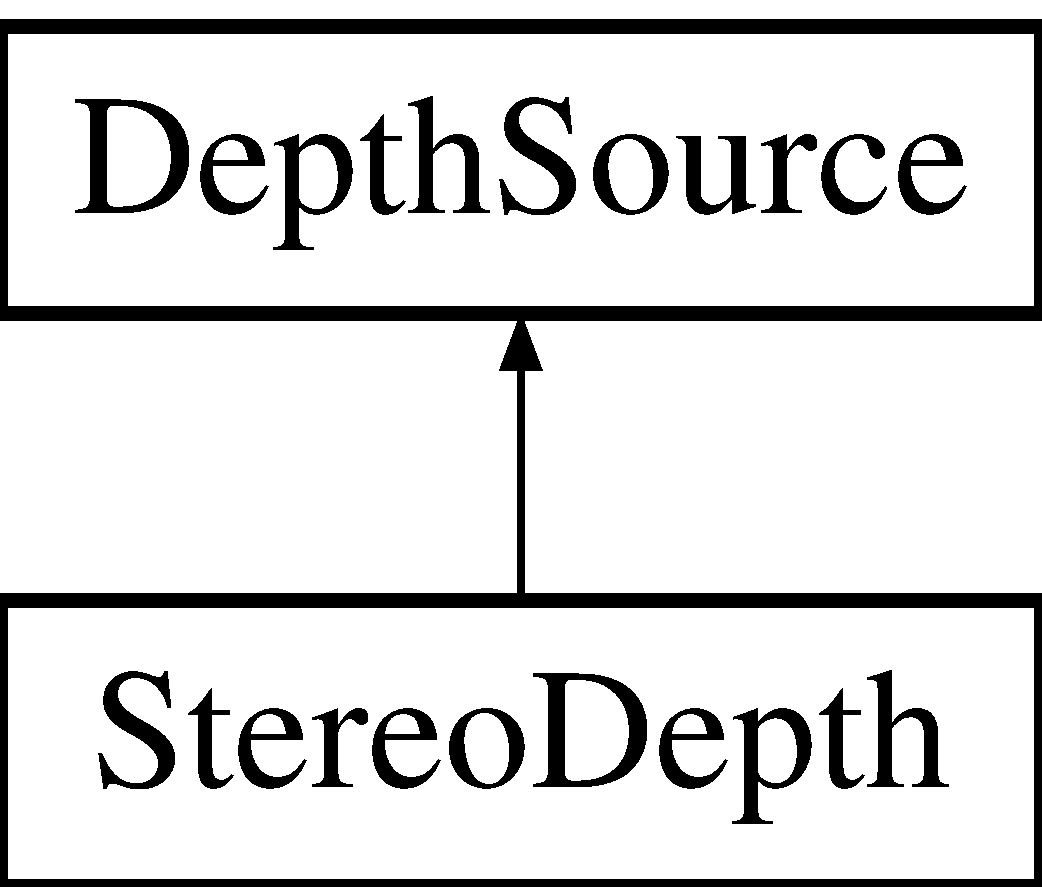
\includegraphics[height=2.000000cm]{classfovis_1_1StereoDepth}
\end{center}
\end{figure}
\subsection*{Public Member Functions}
\begin{DoxyCompactItemize}
\item 
virtual double \hyperlink{classfovis_1_1StereoDepth_a5429ab9acd4e4f8d154c952ff95b1149}{getBaseline} () const 
\item 
virtual void \hyperlink{classfovis_1_1StereoDepth_a0b83e0c45768e90787bc7f0c2c77606d}{getXyz} (\hyperlink{classfovis_1_1OdometryFrame}{OdometryFrame} $\ast$frame)
\item 
virtual bool \hyperlink{classfovis_1_1StereoDepth_ab94d0972d755837688cfc95aa144a6e1}{haveXyz} (int u, int v)
\item 
virtual void \hyperlink{classfovis_1_1StereoDepth_ad0922053f71946f74bc26225848010e6}{refineXyz} (\hyperlink{classfovis_1_1FeatureMatch}{FeatureMatch} $\ast$matches, int num\_\-matches, \hyperlink{classfovis_1_1OdometryFrame}{OdometryFrame} $\ast$frame)
\item 
\hypertarget{classfovis_1_1StereoDepth_a9a80d9547739766e7d8abbb9e2cafb8e}{
void {\bfseries setRightImage} (const uint8\_\-t $\ast$img)}
\label{classfovis_1_1StereoDepth_a9a80d9547739766e7d8abbb9e2cafb8e}

\item 
\hypertarget{classfovis_1_1StereoDepth_ad61e40ec9a733ef28cb90f0593076ca5}{
{\bfseries StereoDepth} (const \hyperlink{classfovis_1_1StereoCalibration}{StereoCalibration} $\ast$calib, const \hyperlink{group__FovisCore_ga113578b67d3e37bc78f1fffd8440e1ff}{VisualOdometryOptions} \&options)}
\label{classfovis_1_1StereoDepth_ad61e40ec9a733ef28cb90f0593076ca5}

\end{DoxyCompactItemize}


\subsection{Detailed Description}
Stores image data for a stereo camera pair. 

TODO 

\subsection{Member Function Documentation}
\hypertarget{classfovis_1_1StereoDepth_ab94d0972d755837688cfc95aa144a6e1}{
\index{fovis::StereoDepth@{fovis::StereoDepth}!haveXyz@{haveXyz}}
\index{haveXyz@{haveXyz}!fovis::StereoDepth@{fovis::StereoDepth}}
\subsubsection[{haveXyz}]{\setlength{\rightskip}{0pt plus 5cm}virtual bool haveXyz (
\begin{DoxyParamCaption}
\item[{int}]{u, }
\item[{int}]{v}
\end{DoxyParamCaption}
)\hspace{0.3cm}{\ttfamily  \mbox{[}virtual\mbox{]}}}}
\label{classfovis_1_1StereoDepth_ab94d0972d755837688cfc95aa144a6e1}
This should return true if it's not certain there's no depth at (u,v). It should be an inexpensive check that is used to avoid pointless (hah!) creation of keypoints. False positives are fine as ling as getXyz gets rid of them. 

Implements \hyperlink{classfovis_1_1DepthSource_ad0d2b9dd0e48e428319c3c84e87fa5cf}{DepthSource}.

\hypertarget{classfovis_1_1StereoDepth_a0b83e0c45768e90787bc7f0c2c77606d}{
\index{fovis::StereoDepth@{fovis::StereoDepth}!getXyz@{getXyz}}
\index{getXyz@{getXyz}!fovis::StereoDepth@{fovis::StereoDepth}}
\subsubsection[{getXyz}]{\setlength{\rightskip}{0pt plus 5cm}virtual void getXyz (
\begin{DoxyParamCaption}
\item[{{\bf OdometryFrame} $\ast$}]{frame}
\end{DoxyParamCaption}
)\hspace{0.3cm}{\ttfamily  \mbox{[}virtual\mbox{]}}}}
\label{classfovis_1_1StereoDepth_a0b83e0c45768e90787bc7f0c2c77606d}
Populate keypoints in frame with XYZ data. 

Implements \hyperlink{classfovis_1_1DepthSource_a0259f77a02ba85f5370407db4759d16a}{DepthSource}.

\hypertarget{classfovis_1_1StereoDepth_ad0922053f71946f74bc26225848010e6}{
\index{fovis::StereoDepth@{fovis::StereoDepth}!refineXyz@{refineXyz}}
\index{refineXyz@{refineXyz}!fovis::StereoDepth@{fovis::StereoDepth}}
\subsubsection[{refineXyz}]{\setlength{\rightskip}{0pt plus 5cm}virtual void refineXyz (
\begin{DoxyParamCaption}
\item[{{\bf FeatureMatch} $\ast$}]{matches, }
\item[{int}]{num\_\-matches, }
\item[{{\bf OdometryFrame} $\ast$}]{frame}
\end{DoxyParamCaption}
)\hspace{0.3cm}{\ttfamily  \mbox{[}virtual\mbox{]}}}}
\label{classfovis_1_1StereoDepth_ad0922053f71946f74bc26225848010e6}
Refine XYZ data of target keypoints in matches (usually after subpixel refinement of the matches across time). 

Implements \hyperlink{classfovis_1_1DepthSource_a4d6eafb84371d0720cd7ee53ac2e659a}{DepthSource}.

\hypertarget{classfovis_1_1StereoDepth_a5429ab9acd4e4f8d154c952ff95b1149}{
\index{fovis::StereoDepth@{fovis::StereoDepth}!getBaseline@{getBaseline}}
\index{getBaseline@{getBaseline}!fovis::StereoDepth@{fovis::StereoDepth}}
\subsubsection[{getBaseline}]{\setlength{\rightskip}{0pt plus 5cm}virtual double getBaseline (
\begin{DoxyParamCaption}
{}
\end{DoxyParamCaption}
) const\hspace{0.3cm}{\ttfamily  \mbox{[}inline, virtual\mbox{]}}}}
\label{classfovis_1_1StereoDepth_a5429ab9acd4e4f8d154c952ff95b1149}
Return baseline of depth source, if applicable. If not applicable (e.g. for OpenNI devices) return 0. 

Implements \hyperlink{classfovis_1_1DepthSource_a22d76295f183f3ec9e34d2d7e837c675}{DepthSource}.



The documentation for this class was generated from the following file:\begin{DoxyCompactItemize}
\item 
stereo\_\-depth.hpp\end{DoxyCompactItemize}

\hypertarget{classfovis_1_1StereoFrame}{
\section{StereoFrame Class Reference}
\label{classfovis_1_1StereoFrame}\index{fovis::StereoFrame@{fovis::StereoFrame}}
}


Stores the right-\/hand image for a stereo pair.  


\subsection*{Public Member Functions}
\begin{DoxyCompactItemize}
\item 
\hypertarget{classfovis_1_1StereoFrame_a3a922a072358cf7d3b82235613f7e129}{
\hyperlink{classfovis_1_1PyramidLevel}{PyramidLevel} $\ast$ {\bfseries getLevel} (int level\_\-num)}
\label{classfovis_1_1StereoFrame_a3a922a072358cf7d3b82235613f7e129}

\item 
\hypertarget{classfovis_1_1StereoFrame_a6b34494d5f8a1666d216bae16f25640b}{
int {\bfseries getNumDetectedKeypoints} () const }
\label{classfovis_1_1StereoFrame_a6b34494d5f8a1666d216bae16f25640b}

\item 
\hypertarget{classfovis_1_1StereoFrame_a3e247d49631478f3ada787127e798de0}{
void {\bfseries prepareFrame} (const uint8\_\-t $\ast$raw\_\-gray, int fast\_\-threshold)}
\label{classfovis_1_1StereoFrame_a3e247d49631478f3ada787127e798de0}

\item 
\hypertarget{classfovis_1_1StereoFrame_a581c51ce9ea9ac8f8488fbf9803055c0}{
void {\bfseries rectify} (Eigen::Vector2d xy\_\-in, Eigen::Vector2d $\ast$out)}
\label{classfovis_1_1StereoFrame_a581c51ce9ea9ac8f8488fbf9803055c0}

\item 
\hypertarget{classfovis_1_1StereoFrame_aa9dff05ab404552e991bef9c4e1c9876}{
{\bfseries StereoFrame} (int width, int height, const \hyperlink{classfovis_1_1Rectification}{Rectification} $\ast$rectify\_\-map, const \hyperlink{group__FovisCore_ga113578b67d3e37bc78f1fffd8440e1ff}{VisualOdometryOptions} \&options)}
\label{classfovis_1_1StereoFrame_aa9dff05ab404552e991bef9c4e1c9876}

\end{DoxyCompactItemize}


\subsection{Detailed Description}
Stores the right-\/hand image for a stereo pair. 

TODO 

The documentation for this class was generated from the following file:\begin{DoxyCompactItemize}
\item 
stereo\_\-frame.hpp\end{DoxyCompactItemize}

\hypertarget{classfovis_1_1VisualOdometry}{
\section{VisualOdometry Class Reference}
\label{classfovis_1_1VisualOdometry}\index{fovis::VisualOdometry@{fovis::VisualOdometry}}
}


Main visual odometry class.  


\subsection*{Public Member Functions}
\begin{DoxyCompactItemize}
\item 
bool \hyperlink{classfovis_1_1VisualOdometry_acbe563757a45cb680db2b6b01f2c1619}{getChangeReferenceFrames} () const 
\item 
int \hyperlink{classfovis_1_1VisualOdometry_aeadd11b0fc7b95fc374f9f4c441cb19b}{getFastThreshold} () const 
\item 
const Eigen::Matrix3d \& \hyperlink{classfovis_1_1VisualOdometry_a06475550bc622f54d1e1152bf48af59d}{getInitialHomography} () const 
\item 
const Eigen::Isometry3d \& \hyperlink{classfovis_1_1VisualOdometry_a7c8a153a489f90c60123666495900a72}{getMotionEstimate} () const 
\item 
const Eigen::MatrixXd \& \hyperlink{classfovis_1_1VisualOdometry_a13c92fba48648f413eebccd6fde24e18}{getMotionEstimateCov} () const 
\item 
MotionEstimateStatusCode \hyperlink{classfovis_1_1VisualOdometry_ae03356861ab491be0d5e608c8cdd33a2}{getMotionEstimateStatus} () const 
\item 
const \hyperlink{classfovis_1_1MotionEstimator}{MotionEstimator} $\ast$ \hyperlink{classfovis_1_1VisualOdometry_a46ee2db8b83c7d29d2788284a20118a5}{getMotionEstimator} () const 
\item 
const \hyperlink{group__FovisCore_ga113578b67d3e37bc78f1fffd8440e1ff}{VisualOdometryOptions} \& \hyperlink{classfovis_1_1VisualOdometry_a1d3dff2d7747af2023d37b9fc083839d}{getOptions} () const 
\item 
const Eigen::Isometry3d \& \hyperlink{classfovis_1_1VisualOdometry_a6e5d8524487f34d5f3c5dc8e26328f81}{getPose} ()
\item 
const \hyperlink{classfovis_1_1OdometryFrame}{OdometryFrame} $\ast$ \hyperlink{classfovis_1_1VisualOdometry_a6700c99d0ce2f67bb76ba55098f0e814}{getReferenceFrame} () const 
\item 
const \hyperlink{classfovis_1_1OdometryFrame}{OdometryFrame} $\ast$ \hyperlink{classfovis_1_1VisualOdometry_a69e5a07d97c47fc049a42f2ba2939cab}{getTargetFrame} () const 
\item 
void \hyperlink{classfovis_1_1VisualOdometry_a58914d47aef477789e434ef7f484d4bb}{processFrame} (const uint8\_\-t $\ast$gray, \hyperlink{classfovis_1_1DepthSource}{DepthSource} $\ast$depth\_\-source)
\item 
void \hyperlink{classfovis_1_1VisualOdometry_a892c8032392efdef960a30a2e8cd817c}{sanityCheck} () const 
\item 
\hyperlink{classfovis_1_1VisualOdometry_a0800e59ff148f215673b02b60a9f1d2c}{VisualOdometry} (const \hyperlink{classfovis_1_1Rectification}{Rectification} $\ast$rectification, const \hyperlink{group__FovisCore_ga113578b67d3e37bc78f1fffd8440e1ff}{VisualOdometryOptions} \&options)
\end{DoxyCompactItemize}
\subsection*{Static Public Member Functions}
\begin{DoxyCompactItemize}
\item 
static \hyperlink{group__FovisCore_ga113578b67d3e37bc78f1fffd8440e1ff}{VisualOdometryOptions} \hyperlink{classfovis_1_1VisualOdometry_a00ae0b1c3d48cf00aebf4b0c820980a9}{getDefaultOptions} ()
\end{DoxyCompactItemize}


\subsection{Detailed Description}
Main visual odometry class. 


\begin{DoxyCode}
 #include <fovis/fovis.hpp>
\end{DoxyCode}


This is the primary fovis class for estimating visual odometry. To use it, you'll need three things: \begin{DoxyItemize}
\item a source of grayscale input images. \item a \hyperlink{classfovis_1_1DepthSource}{DepthSource} that can estimate the distance to as many pixels in the input images as possible. \item a \hyperlink{classfovis_1_1Rectification}{Rectification} object for converting the source image coordinates to a rectified pinhole projection coordinate system. This is typically used to correct radial lens distortion.\end{DoxyItemize}
A typical use case for the \hyperlink{classfovis_1_1VisualOdometry}{VisualOdometry} class is to repeatedly call \hyperlink{classfovis_1_1VisualOdometry_a58914d47aef477789e434ef7f484d4bb}{processFrame()} as new image data is available, which estimates the camera motion and makes the resulting estimation data available via accessor methods.

Options to control the behavior of the visual odometry algorithm can be passed in to the constructor using a VisualOdometryOptions object. 

\subsection{Constructor \& Destructor Documentation}
\hypertarget{classfovis_1_1VisualOdometry_a0800e59ff148f215673b02b60a9f1d2c}{
\index{fovis::VisualOdometry@{fovis::VisualOdometry}!VisualOdometry@{VisualOdometry}}
\index{VisualOdometry@{VisualOdometry}!fovis::VisualOdometry@{fovis::VisualOdometry}}
\subsubsection[{VisualOdometry}]{\setlength{\rightskip}{0pt plus 5cm}{\bf VisualOdometry} (
\begin{DoxyParamCaption}
\item[{const {\bf Rectification} $\ast$}]{rectification, }
\item[{const {\bf VisualOdometryOptions} \&}]{options}
\end{DoxyParamCaption}
)}}
\label{classfovis_1_1VisualOdometry_a0800e59ff148f215673b02b60a9f1d2c}
Constructs a new visual odometry estimator.


\begin{DoxyParams}{Parameters}
{\em rectification} & specifies the input image dimensions, as well as the mapping from input image coordinates to rectified image coordinates. \\
\hline
{\em options} & controls the behavior of the estimation algorithms. This is specified as a key/value dictionary. \\
\hline
\end{DoxyParams}


\subsection{Member Function Documentation}
\hypertarget{classfovis_1_1VisualOdometry_a58914d47aef477789e434ef7f484d4bb}{
\index{fovis::VisualOdometry@{fovis::VisualOdometry}!processFrame@{processFrame}}
\index{processFrame@{processFrame}!fovis::VisualOdometry@{fovis::VisualOdometry}}
\subsubsection[{processFrame}]{\setlength{\rightskip}{0pt plus 5cm}void processFrame (
\begin{DoxyParamCaption}
\item[{const uint8\_\-t $\ast$}]{gray, }
\item[{{\bf DepthSource} $\ast$}]{depth\_\-source}
\end{DoxyParamCaption}
)}}
\label{classfovis_1_1VisualOdometry_a58914d47aef477789e434ef7f484d4bb}
process an input image and estimate the 3D camera motion between {\ttfamily gray} and the frame previously passed to this method. The estimated motion for the very first frame will always be the identity transform.


\begin{DoxyParams}{Parameters}
{\em gray} & a new input image. The image dimensions must match those passed in to the constructor, and the image data must be stored in row-\/major order, with no pad bytes between rows. An internal copy of the image is made, and the input data is no longer needed once this method returns. \\
\hline
{\em depth\_\-source} & a source of depth information that can either provide a depth estimate at each pixel of the input image, or report that no depth estimate is available. \\
\hline
\end{DoxyParams}
\hypertarget{classfovis_1_1VisualOdometry_a6e5d8524487f34d5f3c5dc8e26328f81}{
\index{fovis::VisualOdometry@{fovis::VisualOdometry}!getPose@{getPose}}
\index{getPose@{getPose}!fovis::VisualOdometry@{fovis::VisualOdometry}}
\subsubsection[{getPose}]{\setlength{\rightskip}{0pt plus 5cm}const Eigen::Isometry3d\& getPose (
\begin{DoxyParamCaption}
{}
\end{DoxyParamCaption}
)\hspace{0.3cm}{\ttfamily  \mbox{[}inline\mbox{]}}}}
\label{classfovis_1_1VisualOdometry_a6e5d8524487f34d5f3c5dc8e26328f81}
Retrieves the integrated pose estimate. On initialization, the camera is positioned at the origin, with +Z pointing along the camera look vector, +X to the right, and +Y down. \hypertarget{classfovis_1_1VisualOdometry_a6700c99d0ce2f67bb76ba55098f0e814}{
\index{fovis::VisualOdometry@{fovis::VisualOdometry}!getReferenceFrame@{getReferenceFrame}}
\index{getReferenceFrame@{getReferenceFrame}!fovis::VisualOdometry@{fovis::VisualOdometry}}
\subsubsection[{getReferenceFrame}]{\setlength{\rightskip}{0pt plus 5cm}const {\bf OdometryFrame}$\ast$ getReferenceFrame (
\begin{DoxyParamCaption}
{}
\end{DoxyParamCaption}
) const\hspace{0.3cm}{\ttfamily  \mbox{[}inline\mbox{]}}}}
\label{classfovis_1_1VisualOdometry_a6700c99d0ce2f67bb76ba55098f0e814}
Retrieve the current reference frame used for motion estimation. The reference frame will not change as long as new input frames are easily matched to it. \hypertarget{classfovis_1_1VisualOdometry_a69e5a07d97c47fc049a42f2ba2939cab}{
\index{fovis::VisualOdometry@{fovis::VisualOdometry}!getTargetFrame@{getTargetFrame}}
\index{getTargetFrame@{getTargetFrame}!fovis::VisualOdometry@{fovis::VisualOdometry}}
\subsubsection[{getTargetFrame}]{\setlength{\rightskip}{0pt plus 5cm}const {\bf OdometryFrame}$\ast$ getTargetFrame (
\begin{DoxyParamCaption}
{}
\end{DoxyParamCaption}
) const\hspace{0.3cm}{\ttfamily  \mbox{[}inline\mbox{]}}}}
\label{classfovis_1_1VisualOdometry_a69e5a07d97c47fc049a42f2ba2939cab}
Retrieve the current target frame used for motion estimation. \hypertarget{classfovis_1_1VisualOdometry_acbe563757a45cb680db2b6b01f2c1619}{
\index{fovis::VisualOdometry@{fovis::VisualOdometry}!getChangeReferenceFrames@{getChangeReferenceFrames}}
\index{getChangeReferenceFrames@{getChangeReferenceFrames}!fovis::VisualOdometry@{fovis::VisualOdometry}}
\subsubsection[{getChangeReferenceFrames}]{\setlength{\rightskip}{0pt plus 5cm}bool getChangeReferenceFrames (
\begin{DoxyParamCaption}
{}
\end{DoxyParamCaption}
) const\hspace{0.3cm}{\ttfamily  \mbox{[}inline\mbox{]}}}}
\label{classfovis_1_1VisualOdometry_acbe563757a45cb680db2b6b01f2c1619}
If this returns true, then the current target frame will become the reference frame on the next call to \hyperlink{classfovis_1_1VisualOdometry_a58914d47aef477789e434ef7f484d4bb}{processFrame()}. \hypertarget{classfovis_1_1VisualOdometry_ae03356861ab491be0d5e608c8cdd33a2}{
\index{fovis::VisualOdometry@{fovis::VisualOdometry}!getMotionEstimateStatus@{getMotionEstimateStatus}}
\index{getMotionEstimateStatus@{getMotionEstimateStatus}!fovis::VisualOdometry@{fovis::VisualOdometry}}
\subsubsection[{getMotionEstimateStatus}]{\setlength{\rightskip}{0pt plus 5cm}MotionEstimateStatusCode getMotionEstimateStatus (
\begin{DoxyParamCaption}
{}
\end{DoxyParamCaption}
) const\hspace{0.3cm}{\ttfamily  \mbox{[}inline\mbox{]}}}}
\label{classfovis_1_1VisualOdometry_ae03356861ab491be0d5e608c8cdd33a2}
\begin{DoxyReturn}{Returns}
whether motion estimation succeeded on the most recent call to \hyperlink{classfovis_1_1VisualOdometry_a58914d47aef477789e434ef7f484d4bb}{processFrame()}, or provides a rough failure reason. 
\end{DoxyReturn}
\hypertarget{classfovis_1_1VisualOdometry_a7c8a153a489f90c60123666495900a72}{
\index{fovis::VisualOdometry@{fovis::VisualOdometry}!getMotionEstimate@{getMotionEstimate}}
\index{getMotionEstimate@{getMotionEstimate}!fovis::VisualOdometry@{fovis::VisualOdometry}}
\subsubsection[{getMotionEstimate}]{\setlength{\rightskip}{0pt plus 5cm}const Eigen::Isometry3d\& getMotionEstimate (
\begin{DoxyParamCaption}
{}
\end{DoxyParamCaption}
) const\hspace{0.3cm}{\ttfamily  \mbox{[}inline\mbox{]}}}}
\label{classfovis_1_1VisualOdometry_a7c8a153a489f90c60123666495900a72}
\begin{DoxyReturn}{Returns}
the estimated camera motion from the previous frame to the current frame. 
\end{DoxyReturn}
\hypertarget{classfovis_1_1VisualOdometry_a13c92fba48648f413eebccd6fde24e18}{
\index{fovis::VisualOdometry@{fovis::VisualOdometry}!getMotionEstimateCov@{getMotionEstimateCov}}
\index{getMotionEstimateCov@{getMotionEstimateCov}!fovis::VisualOdometry@{fovis::VisualOdometry}}
\subsubsection[{getMotionEstimateCov}]{\setlength{\rightskip}{0pt plus 5cm}const Eigen::MatrixXd\& getMotionEstimateCov (
\begin{DoxyParamCaption}
{}
\end{DoxyParamCaption}
) const\hspace{0.3cm}{\ttfamily  \mbox{[}inline\mbox{]}}}}
\label{classfovis_1_1VisualOdometry_a13c92fba48648f413eebccd6fde24e18}
\begin{DoxyReturn}{Returns}
the covariance matrix resulting from the final nonlinear least-\/squares motion estimation step. 
\end{DoxyReturn}
\hypertarget{classfovis_1_1VisualOdometry_a46ee2db8b83c7d29d2788284a20118a5}{
\index{fovis::VisualOdometry@{fovis::VisualOdometry}!getMotionEstimator@{getMotionEstimator}}
\index{getMotionEstimator@{getMotionEstimator}!fovis::VisualOdometry@{fovis::VisualOdometry}}
\subsubsection[{getMotionEstimator}]{\setlength{\rightskip}{0pt plus 5cm}const {\bf MotionEstimator}$\ast$ getMotionEstimator (
\begin{DoxyParamCaption}
{}
\end{DoxyParamCaption}
) const\hspace{0.3cm}{\ttfamily  \mbox{[}inline\mbox{]}}}}
\label{classfovis_1_1VisualOdometry_a46ee2db8b83c7d29d2788284a20118a5}
\begin{DoxyReturn}{Returns}
the \hyperlink{classfovis_1_1MotionEstimator}{MotionEstimator} object used internally. 
\end{DoxyReturn}
\hypertarget{classfovis_1_1VisualOdometry_aeadd11b0fc7b95fc374f9f4c441cb19b}{
\index{fovis::VisualOdometry@{fovis::VisualOdometry}!getFastThreshold@{getFastThreshold}}
\index{getFastThreshold@{getFastThreshold}!fovis::VisualOdometry@{fovis::VisualOdometry}}
\subsubsection[{getFastThreshold}]{\setlength{\rightskip}{0pt plus 5cm}int getFastThreshold (
\begin{DoxyParamCaption}
{}
\end{DoxyParamCaption}
) const\hspace{0.3cm}{\ttfamily  \mbox{[}inline\mbox{]}}}}
\label{classfovis_1_1VisualOdometry_aeadd11b0fc7b95fc374f9f4c441cb19b}
\begin{DoxyReturn}{Returns}
the threshold used by the FAST feature detector. 
\end{DoxyReturn}
\hypertarget{classfovis_1_1VisualOdometry_a06475550bc622f54d1e1152bf48af59d}{
\index{fovis::VisualOdometry@{fovis::VisualOdometry}!getInitialHomography@{getInitialHomography}}
\index{getInitialHomography@{getInitialHomography}!fovis::VisualOdometry@{fovis::VisualOdometry}}
\subsubsection[{getInitialHomography}]{\setlength{\rightskip}{0pt plus 5cm}const Eigen::Matrix3d\& getInitialHomography (
\begin{DoxyParamCaption}
{}
\end{DoxyParamCaption}
) const\hspace{0.3cm}{\ttfamily  \mbox{[}inline\mbox{]}}}}
\label{classfovis_1_1VisualOdometry_a06475550bc622f54d1e1152bf48af59d}
\begin{DoxyReturn}{Returns}
the 2D homography computed during initial rotation estimation. 
\end{DoxyReturn}
\hypertarget{classfovis_1_1VisualOdometry_a1d3dff2d7747af2023d37b9fc083839d}{
\index{fovis::VisualOdometry@{fovis::VisualOdometry}!getOptions@{getOptions}}
\index{getOptions@{getOptions}!fovis::VisualOdometry@{fovis::VisualOdometry}}
\subsubsection[{getOptions}]{\setlength{\rightskip}{0pt plus 5cm}const {\bf VisualOdometryOptions}\& getOptions (
\begin{DoxyParamCaption}
{}
\end{DoxyParamCaption}
) const\hspace{0.3cm}{\ttfamily  \mbox{[}inline\mbox{]}}}}
\label{classfovis_1_1VisualOdometry_a1d3dff2d7747af2023d37b9fc083839d}
\begin{DoxyReturn}{Returns}
the options passed in to the constructor. 
\end{DoxyReturn}
\hypertarget{classfovis_1_1VisualOdometry_a00ae0b1c3d48cf00aebf4b0c820980a9}{
\index{fovis::VisualOdometry@{fovis::VisualOdometry}!getDefaultOptions@{getDefaultOptions}}
\index{getDefaultOptions@{getDefaultOptions}!fovis::VisualOdometry@{fovis::VisualOdometry}}
\subsubsection[{getDefaultOptions}]{\setlength{\rightskip}{0pt plus 5cm}static {\bf VisualOdometryOptions} getDefaultOptions (
\begin{DoxyParamCaption}
{}
\end{DoxyParamCaption}
)\hspace{0.3cm}{\ttfamily  \mbox{[}static\mbox{]}}}}
\label{classfovis_1_1VisualOdometry_a00ae0b1c3d48cf00aebf4b0c820980a9}
\begin{DoxyReturn}{Returns}
a reasonable set of default options that can be passed in to the constructor if you don't know or care about the options. 
\end{DoxyReturn}
\hypertarget{classfovis_1_1VisualOdometry_a892c8032392efdef960a30a2e8cd817c}{
\index{fovis::VisualOdometry@{fovis::VisualOdometry}!sanityCheck@{sanityCheck}}
\index{sanityCheck@{sanityCheck}!fovis::VisualOdometry@{fovis::VisualOdometry}}
\subsubsection[{sanityCheck}]{\setlength{\rightskip}{0pt plus 5cm}void sanityCheck (
\begin{DoxyParamCaption}
{}
\end{DoxyParamCaption}
) const}}
\label{classfovis_1_1VisualOdometry_a892c8032392efdef960a30a2e8cd817c}
Performs some internal sanity checks and aborts the program on failure. This is for debugging only. 

The documentation for this class was generated from the following file:\begin{DoxyCompactItemize}
\item 
visual\_\-odometry.hpp\end{DoxyCompactItemize}

\chapter{File Documentation}
\hypertarget{options_8hpp}{
\section{options.hpp File Reference}
\label{options_8hpp}\index{options.hpp@{options.hpp}}
}


Options.  


\subsection*{Typedefs}
\begin{DoxyCompactItemize}
\item 
typedef std::map$<$ std::string, std::string $>$ \hyperlink{group__FovisCore_ga113578b67d3e37bc78f1fffd8440e1ff}{VisualOdometryOptions}
\begin{DoxyCompactList}\small\item\em Options. \end{DoxyCompactList}\end{DoxyCompactItemize}


\subsection{Detailed Description}
Options. TODO 
\printindex
\end{document}
